%%
%% This is file `sample-sigconf.tex',
%% generated with the docstrip utility.
%%
%% The original source files were:
%%
%% samples.dtx  (with options: `all,proceedings,bibtex,sigconf')
%% 
%% IMPORTANT NOTICE:
%% 
%% For the copyright see the source file.
%% 
%% Any modified versions of this file must be renamed
%% with new filenames distinct from sample-sigconf.tex.
%% 
%% For distribution of the original source see the terms
%% for copying and modification in the file samples.dtx.
%% 
%% This generated file may be distributed as long as the
%% original source files, as listed above, are part of the
%% same distribution. (The sources need not necessarily be
%% in the same archive or directory.)
%%
%%
%% Commands for TeXCount
%TC:macro \cite [option:text,text]
%TC:macro \citep [option:text,text]
%TC:macro \citet [option:text,text]
%TC:envir table 0 1
%TC:envir table* 0 1
%TC:envir tabular [ignore] word
%TC:envir displaymath 0 word
%TC:envir math 0 word
%TC:envir comment 0 0
%%
%% The first command in your LaTeX source must be the \documentclass
%% command.
%%
%% For submission and review of your manuscript please change the
%% command to \documentclass[manuscript, screen, review]{acmart}.
%%
%% When submitting camera ready or to TAPS, please change the command
%% to \documentclass[sigconf]{acmart} or whichever template is required
%% for your publication.
%%
%%
\documentclass[manuscript,screen,review,anonymous]{acmart}
\usepackage{amssymb}
\usepackage{siunitx}
\PassOptionsToPackage{hyphens}{url}\usepackage{hyperref}
\usepackage{cleveref}
\usepackage[utf8]{inputenc}
\usepackage[right]{lineno}
\usepackage{csquotes}
\usepackage{booktabs}
\usepackage{subcaption}
\usepackage{longtable}
\usepackage{adjustbox}
\usepackage{xcolor,colortbl}  % For cell colors
\usepackage{multirow}          % For spanning headers (optional)
\usepackage{array}
\usepackage{url}
%\usepackage{titlesec}
%\usepackage[compatibility=false]{caption}
\usepackage{authblk}
\usepackage{xcolor} % Load the xcolor package for color options
%\renewcommand{\thetable}{\Roman{table}}
\usepackage{tabularx}
\definecolor{changeblue}{RGB}{0,0,255}

\newif\ifshowchanges
% \showchangestrue

\ifshowchanges
  \DeclareRobustCommand{\change}[1]{%
    \textcolor{changeblue}{#1}%
  }
\else
  \DeclareRobustCommand{\change}[1]{#1}
\fi
%% \BibTeX command to typeset BibTeX logo in the docs
\AtBeginDocument{%
  \providecommand\BibTeX{{%
    Bib\TeX}}}

%% Rights management information.  This information is sent to you
%% when you complete the rights form.  These commands have SAMPLE
%% values in them; it is your responsibility as an author to replace
%% the commands and values with those provided to you when you
%% complete the rights form.
\setcopyright{acmlicensed}
\copyrightyear{2026}
\acmYear{2026}
\acmDOI{XXXXXXX.XXXXXXX}
%% These commands are for a PROCEEDINGS abstract or paper.
\acmConference[CUI '26]{ACM conference on Conversational User Interfaces}{July 21--24,
  2026}{Bremen, Germany}
%%
%%  Uncomment \acmBooktitle if the title of the proceedings is different
%%  from ``Proceedings of ...''!
%%
%%\acmBooktitle{Woodstock '18: ACM Symposium on Neural Gaze Detection,
%%  June 03--05, 2018, Woodstock, NY}
\acmISBN{978-1-4503-XXXX-X/2026/07}


%%
%% Submission ID.
%% Use this when submitting an article to a sponsored event. You'll
%% receive a unique submission ID from the organizers
%% of the event, and this ID should be used as the parameter to this command.
%%\acmSubmissionID{123-A56-BU3}

%%
%% For managing citations, it is recommended to use bibliography
%% files in BibTeX format.
%%
%% You can then either use BibTeX with the ACM-Reference-Format style,
%% or BibLaTeX with the acmnumeric or acmauthoryear sytles, that include
%% support for advanced citation of software artefact from the
%% biblatex-software package, also separately available on CTAN.
%%
%% Look at the sample-*-biblatex.tex files for templates showcasing
%% the biblatex styles.
%%

%%
%% The majority of ACM publications use numbered citations and
%% references.  The command \citestyle{authoryear} switches to the
%% "author year" style.
%%
%% If you are preparing content for an event
%% sponsored by ACM SIGGRAPH, you must use the "author year" style of
%% citations and references.
%% Uncommenting
%% the next command will enable that style.
%%\citestyle{acmauthoryear}


%%
%% end of the preamble, start of the body of the document source.
\begin{document}

%%
%% The "title" command has an optional parameter,
%% allowing the author to define a "short title" to be used in page headers.
%\title{The Effects of Anthropomorphism in Conversational Agents: A Meta-Analysis}
%\title{The Seven Consequences of Anthropomorphism in Conversational Agents: A Meta-Analysis}
%\title[The Effects of Anthropomorphism in Conversational Agents]{The Effects of Anthropomorphism in Conversational Agents on User Outcomes: A Meta-Analysis}
\title[Anthropomorphic Attributes for Conversational Agents]{How to Design Anthropomorphic Attributes for Conversational Agents?: A Meta Analysis of 79 Articles}


\begin{abstract}

Anthropomorphic design in conversational agents (CA) is of prime importance \change{influencing social perception, satisfaction, and engagement} of user interaction. However, the field lacks clear guidance on which types of anthropomorphic attributes are most important. \change{We extracted 583 effects from 79 studies (2018--2025) and conducted a random-effects meta-analysis on the 169 effects with calculable statistics (N = 21,104), supplementing these with complementary synthesis methods for the remaining 373 directional effects,} examining how anthropomorphic attributes (behavioral vs. demographic) affect user outcomes, such as user experience (UX), trust, and credibility. The results show that behavioral attributes, such as communication style, personality traits, and responsiveness, create stronger effects on user outcomes than demographic attributes, such as demographic identity and visual appearance. We observe large effects of anthropomorphism on social perception and UX, and moderate effects on trust and learning. Our findings suggest that developers of CAs should prioritize how CAs communicate and behave over how they look or who they represent.

\end{abstract}

\keywords{Conversational agents; Anthropomorphism; Meta-analysis; User Outcomes; Human-AI interaction}

%%
%% The code below is generated by the tool at http://dl.acm.org/ccs.cfm.
%% Please copy and paste the code instead of the example below.
%%
% \begin{CCSXML}
% <ccs2012>
%  <concept>
%   <concept_id>00000000.0000000.0000000</concept_id>
%   <concept_desc>Do Not Use This Code, Generate the Correct Terms for Your Paper</concept_desc>
%   <concept_significance>500</concept_significance>
%  </concept>
%  <concept>
%   <concept_id>00000000.00000000.00000000</concept_id>
%   <concept_desc>Do Not Use This Code, Generate the Correct Terms for Your Paper</concept_desc>
%   <concept_significance>300</concept_significance>
%  </concept>
%  <concept>
%   <concept_id>00000000.00000000.00000000</concept_id>
%   <concept_desc>Do Not Use This Code, Generate the Correct Terms for Your Paper</concept_desc>
%   <concept_significance>100</concept_significance>
%  </concept>
%  <concept>
%   <concept_id>00000000.00000000.00000000</concept_id>
%   <concept_desc>Do Not Use This Code, Generate the Correct Terms for Your Paper</concept_desc>
%   <concept_significance>100</concept_significance>
%  </concept>
% </ccs2012>
% \end{CCSXML}

% \ccsdesc[500]{Do Not Use This Code~Generate the Correct Terms for Your Paper}
% \ccsdesc[300]{Do Not Use This Code~Generate the Correct Terms for Your Paper}
% \ccsdesc{Do Not Use This Code~Generate the Correct Terms for Your Paper}
% \ccsdesc[100]{Do Not Use This Code~Generate the Correct Terms for Your Paper}

% %%
% %% Keywords. The author(s) should pick words that accurately describe
% %% the work being presented. Separate the keywords with commas.
% \keywords{Do, Not, Use, This, Code, Put, the, Correct, Terms, for,
%   Your, Paper}
%% A "teaser" image appears between the author and affiliation
%% information and the body of the document, and typically spans the
%% page.
% \begin{teaserfigure}
%   
\includegraphics[width=\textwidth]{sampleteaser}
%   \caption{Seattle Mariners at Spring Training, 2010.}
%   \Description{Enjoying the baseball game from the third-base
%   seats. Ichiro Suzuki preparing to bat.}
%   \label{fig:teaser}
% \end{teaserfigure}

% \received{20 February 2007}
% \received[revised]{12 March 2009}
% \received[accepted]{5 June 2009}

%%
%% This command processes the author and affiliation and title
%% information and builds the first part of the formatted document.
\maketitle

\section{Introduction}
\label{sec:introduction}

Conversational agents (CAs), commonly referred to as chatbots, virtual assistants, virtual companions, or embodied agents \citep{klein_effects_2025}, are software systems that interact with users through natural language using text or voice interfaces \citep{diederich_conversational_2019}. Examples include Alexa, ChatGPT, Cortana, and Siri. These systems employ natural language processing (NLP), machine learning (ML), and large language models (LLMs) to understand user inputs and generate responses. CAs serve critical functions in areas such as customer service, healthcare, education, and social companionship \citep{araujo2018living,brandtzaeg2017people}.

%Counterintuitively, human-like CAs may not necessarily be the most effective in `appearing human' to users. 
%Adding human attributes (e.g., faces, names, demographics) may humanize CAs; however, some studies suggest that users respond more genuinely to how an agent communicates than to how it appears. CA social cues trigger social responses in users \cite{nass1994computers, nass2000machines}, and users' perceived humanness leads to trust and engagement \cite{gunawardena1995social}. These insights indicate that conversational aspects (e.g., tone, politeness, responsiveness) may elicit social reactions beyond visual characteristics of CAs. If anthropomorphism relies more on conversational than visual aspects, then existing CA design may be misaligned with objectives. This conundrum raises a motivational question: \textit{which CA anthropomorphic attributes actually drive user outcomes?}

The design of these CA systems, particularly whether to assign human-like characteristics, referred to as \textit{anthropomorphism}, is a critical decision affecting factors such as user acceptance, system effectiveness \citep{pfeuffer2019anthropomorphic,ashfaq2020deploying}, and engagement \citep{gong_how_2008}. As Chandra et al. \cite{chandra_be_2022} argue, ``the business impact of conversational AI is contingent on customers using and adequately engaging with these tools'' (p. 969). Developments in LLMs exemplify the importance of anthropomorphism for engagement; for instance, OpenAI describes ChatGPT 5.1 as ``warmer'' and ``having more personality'' \citep{hayden_field_openai_2025}, demonstrating focus on anthropomorphic attributes. Given that ChatGPT has more than 900M weekly active users as of December 2025\footnote{\url{https://backlinko.com/chatgpt-stats}}, it is evident that the anthropomorphic design choices in CAs command an immense global impact on conversational system usage.

\begin{figure*}[htbp]
    \centering
    \begin{subfigure}[b]{0.33\textwidth}
        \centering
        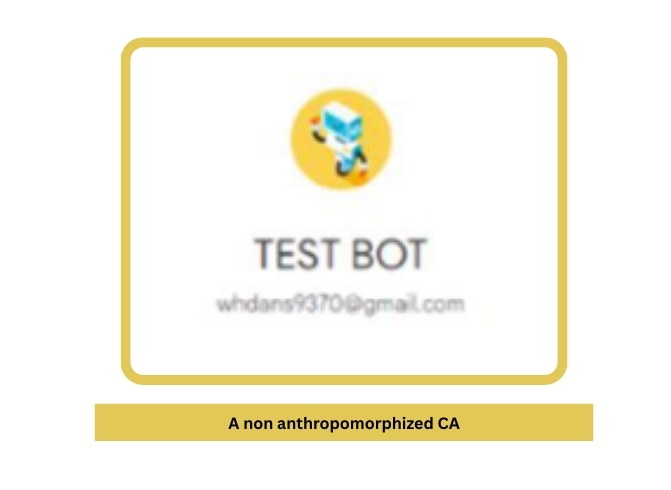
\includegraphics[width=0.75\textwidth]{Figures/12.jpg}
        \caption{Non-anthropomorphic CA}
        \label{fig:ca_nonhuman}
    \end{subfigure}
    \hfill
    \begin{subfigure}[b]{0.33\textwidth}
        \centering
        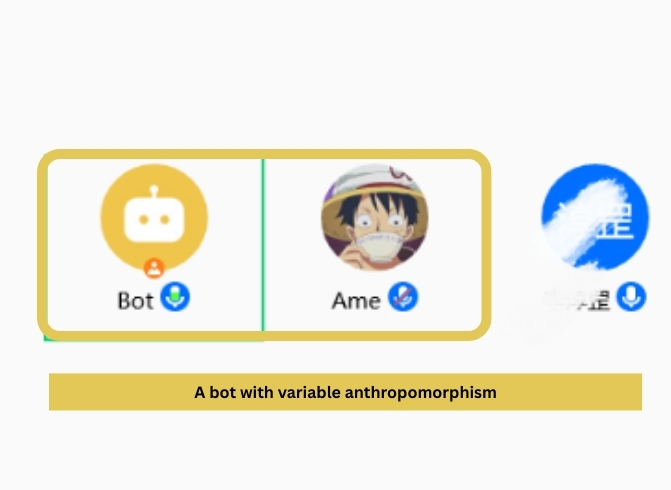
\includegraphics[width=0.75\textwidth]{Figures/14.jpg}
        \caption{A CA with variable anthropomorphism}
        \label{fig:ca_nonhuman}
    \end{subfigure}
    \hfill
    \begin{subfigure}[b]{0.33\textwidth}
        \centering
        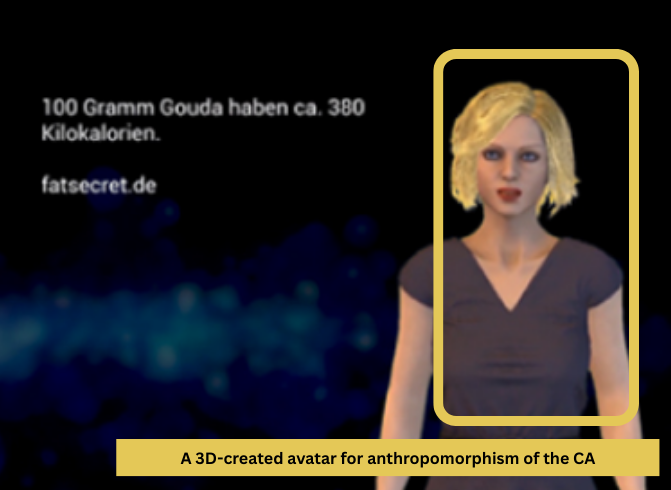
\includegraphics[width=0.75\textwidth]{Figures/13.png}
        \caption{Anthropomorphized CA with 3D avatar}
        \label{fig:ca_human}
    \end{subfigure}
    \caption{\textbf{Anthropomorphism in conversational agents.} Examples show (a) a non-anthropomorphic CA and (b) an anthropomorphic CA with variable anthropomorphism and (c) a anthropomorphized CA with a 3D avatar.}
    \label{fig:CAs}
\end{figure*}

Anthropomorphism in CAs (see examples in Figure \ref{fig:CAs}) usually involves assigning human characteristics such as names, personality traits, appearances, and conversational styles \citep{epley2007seeing,klein_effects_2025}. Research has expanded rapidly since the introduction of LLMs \citep{chen2024trends}, examining CAs' effects on conversation fluency, user experience (UX), and interaction outcomes. Some research demonstrates that anthropomorphic attributes increase trust through social presence \citep{konya2023anthropomorphism,blut2021understanding}, while other studies identify negative effects, such as human-like characteristics creating unrealistic expectations \citep{crolic2022blame,ciechanowski2019shades}.

Despite growing interest, a \textit{systematic understanding of which anthropomorphic attributes matter for user outcomes, such as UX, satisfaction, and trust, remains lacking}. We define user outcomes as any measurable user response to CA interactions, including perceptions, attitudes, behaviors, and performance. Studies examine individual characteristics, such as names \citep{go2019humanizing}, gender, communication style \citep{seeger2021texting}, but findings remain scattered, and people using conversational interfaces lack evidence-based guidance to design anthropomorphically optimal CAs. %For example, trust formation is a primary concern, as users must decide whether to accept CAs \citep{meyer2023leverage,følstad2021chatbots,nordheim2019trust}. 
Without the synthesis of anthropomorphic CA attributes, implementation methods, and user outcomes, CA developers are inclined to make design choices based on intuition instead of validated research.

Prior meta-analyses have %examined human-like cues in conversational agents. Chaves and Gerosa \cite{chaves2021should} reviewed 56 articles to analyze how social characteristics influence human–chatbot interactions, finding 
found that certain CA characteristics are domain-dependent (e.g., moral agency, communicability), whereas others apply broadly across contexts (e.g., manners, damage control) \cite{chaves2021should}. Klein \cite{klein_effects_2025} synthesized 142 studies on human-like social cues in text-based conversational agents, reporting a small-to-medium effect ($g$ = 0.36) on social responses. They identified variability across anthropomorphic attributes and outcome measures, though the study focused exclusively on text-based interactions. 

Building on this foundation, we extend the body of knowledge on anthropomorphic design of CAs by examining anthropomorphic attributes across all CA modalities (text, voice, embodied), distinguishing between behavioral (communication style, personality, responsiveness) and demographic attributes (demographic identity, role, visual appearance). %, and employing hybrid synthesis methods to maximize data utilization.
To this end, our meta-analysis addresses the following research question: 
\textit{How do anthropomorphic attributes of conversational agents affect user outcomes?} 
To address this question, we synthesize empirical findings from 79 articles (2018-2025), organizing results by outcome categories and identifying which specific attributes produce consistent effects. Our analysis focuses on a meta-analysis of 583 effects (N = 21,104). % with qualitative synthesis methods (365 additional effects), achieving 93\% data utilization through vote counting \cite{votecounting}, Fisher's combined probability test, and Stouffer's Z-score methods.

Understanding how anthropomorphic attributes affect user outcomes is essential for CA design. Research reports effects on trust and acceptance \citep{kraus_role_2021,chandra_be_2022}, UX \citep{lieb_student_2024,liu_older_2023}, behavioral patterns \citep{mehra_chatbot_2021,chen_you_2021}, and task performance \citep{zheldibayeva_genai_2025,baihaqi_rapport-driven_2024}. However, findings are scattered. Our synthesis organizes these empirical findings into outcome categories and identifies conditions under which anthropomorphic design produces effects.
By doing so, the current study makes several contributions to conversational user interface research. \change{First, we  derive a behavioral–demographic taxonomy of anthropomorphic attributes through hierarchical agglomerative clustering of co-occurrence patterns across 79 studies.} Second, we demonstrate that behavioral attributes produce substantially stronger effects than demographic attributes, with overall moderate effects approximately twice the magnitude of prior text-only meta-analyses. Third, we compare findings across several user outcome categories, finding the strongest effects for social perception and UX. Fourth, we provide design guidelines for CA developers to design anthropomorphic CAs.
% These findings suggest that CA developers should prioritize natural communication patterns and personality coherence over demographic or visual cues when designing anthropomorphic CAs.

\section{Related Work}

% --- Section 2.1: Broad IS Context (Preserved your original text) ---
\subsection{Brief History of Conversational Agents}
CAs have existed for several decades, since at least Weizenbaum's \texttt{ELIZA} in 1966, which simulated a psychotherapist \citep{weizenbaum_elizacomputer_1966}\footnote{Before that, Alan Turing had discussed the prospect of a machine imitating humans in conversations in his seminal article from 1950 \citep{turing_computing_1950}.}. Despite having been studied for decades, only the LLM technology has brought about a decisive breakthrough in the abilities of CAs to carry out conversations with human users. Peter et al. \cite{peter_benefits_2025} use the term ``anthropomorphic conversational agents'' to characterize recent LLMs that, despite lacking genuine social understanding, excel at simulating empathy and persuasion to a degree that renders them nearly indistinguishable from real people. %Now, even though CAs have been studied extensively in fields like HCI and NLP, investigating anthropomorphism or ``human-likeness'' as a means to improve user engagement with CAs deviates from most earlier IS user engagement research, which has largely centered on the functional or instrumental value of information technology \citep{chandra_be_2022}. For this reason, it is worthwhile to discuss the nature of CAs as forms of IS.

Overall, %CAs function as interactive UIs that collect, process, and disseminate information through natural language \citep{nguyen2024conversational,mariani2023artificial,pfeuffer2019anthropomorphic}.
% Because natural language can be either written or spoken, CAs communicate with users through text, speech, or a combination of both \citep{diederich_conversational_2019}. 
% Furthermore, 
CAs can be categorized into (1) text-based CAs (written text only, no embodiment\footnote{Embodiment refers to the physical or visual representation of a CA, such as an avatar or robot body. While embodiment is one possible anthropomorphic attribute, anthropomorphism is a broader concept encompassing any human-like characteristic including name, personality, communication style, and behavior.}), (2) virtual CAs (written and spoken interaction with virtual interactive avatars), (3) speech-based CAs (spoken interaction without embodiment), and (4) physical CAs (spoken interaction with physical embodiment) \citep{diederich_design_2022}. 
Across these CA types, a shared trait is the reliance on natural language for interaction \citep{diederich_design_2022}. 
Another key trait of CAs is that, unlike navigation-based UIs, CAs adapt to user needs \citep{folstad2017chatbots,jain2018evaluating}. For example, a student can ask a CA for steps to solve a mathematics problem, and the CA will provide them. A CA can take multiple forms, including static or interactive virtual avatars, physical embodiments, or a disembodied form based solely on natural language \citep{diederich_conversational_2019,diederich_design_2022}. These different implementations shape how users perceive the CA \citep{peter_benefits_2025}, while making systems and information more accessible. Peter et al. \cite{peter_benefits_2025} even argue that one of the core objectives of computer science is ``to make computers more accessible and more natural to interact with, \textit{by making computing more human-like}'' (p. 1, emphasis by us). Chaves and Gerosa \cite{chaves2021should} further emphasize the role of interaction design by postulating that ``making a conversational agent acceptable to users is primarily a social, not only technical, problem'' (p. 729). These conceptual underpinnings have prompted researchers to theorize about anthropomorphism in computer systems and CAs, in particular.

% To this end, modern CAs are widely diffused. They integrate both with enterprise and consumer IS, including customer relationship management (CRM) systems and knowledge management platforms \citep{mariani2023artificial}, technical support, customer service, and social media \citep{diederich_design_2022,schuetzler_impact_2020}, among other types of IS. While CAs were historically viewed as passive retrieval tools, modern CAs, enabled by LLMs, not only fetch information but can also interpret it, making them active agents in the information flow from systems to users \citep{allouch2021conversational}. 
% % --- Added Transition to Anthropomorphism ---
% However, as CAs take on these active roles, the distinction between ``system'' and ``social actor'' blurs. This shift calls for a deeper understanding of how the design of the CA itself, through its humanization, impacts the interaction between the user and the system.

\subsection{Theories of Anthropomorphism in Software Systems}

%Anthropomorphism, the attribution of human characteristics, emotions, or behaviors to non-human entities, draws on the CASA paradigm, which posits that users unconsciously apply social rules to technology \citep{nass1994computers}. Anthropomorphism is a critical component in CAs, because ``[user] engagement [with CAs] depends, in turn, on conversational AI’s similarity, or likeness to the human beings it is intended to replace'' \citep{chandra_be_2022} (p. 969).

The theoretical foundation for understanding why users respond socially to CAs can be derived from the ``\textbf{C}omputers \textbf{A}re \textbf{S}ocial \textbf{A}ctors'' (CASA) paradigm \cite{nass2000researching}. Introduced by Nass et al. \cite{nass1994computers}, CASA argues that humans apply social rules to computers even when they know they are interacting with machines. The key insight is that social responses to computers ``are automatic and
unconscious'' (p. 77) \citep{nass1994computers}. When computers display social cues such as language or voice, users automatically apply human interaction behaviors that include, for example, (1) gender stereotyping (e.g., rating female-voiced computers as more knowledgeable about relationships), (2) reciprocity (e.g., feeling obliged to help a computer that provided assistance), and (3) politeness norms (e.g., giving more favorable evaluations when the computer itself asks for feedback) \citep{nass1997machines}. 

A related concept is \textit{social presence}, which refers to ``the degree of salience of the other person in the interaction'' (p. 65) \citep{short1976social}. In the CA context, social presence captures the extent to which users perceive the agent as a real social entity instead of merely a tool \citep{oh2018systematic}. While CASA explains the automatic process of applying social rules, social presence addresses the sense of interacting with another being. Social presence is associated with increased trust and engagement \citep{gunawardena1995social}. Prior research \cite{gambino2020building,koger2023casa} %raises questions about whether CASA effects persist as users become familiar with technology. Gambino et al. \cite{gambino2020building} proposed extending CASA, arguing that users may develop distinct human-media scripts over time. Furthermore, a replication study found that participants no longer responded socially to desktop computers after 30 years of exposure \citep{koger2023casa}. This 
suggests that CASA effects may wane over time and be strongest for emerging technologies, such as LLM-based CAs. CASA also implies that even minimal anthropomorphic cues can trigger social responses. For example, Araujo \cite{araujo2018living} showed that the \change{simply} assigning the CA a name can increase users' perception of the agent's human-likeness. Therefore, the question is not whether to anthropomorphize or not, but \textit{how}.  %, thus motivating RQ1 and RQ2. These aspects have thus far eluded mainstream research in IS; as eloquently put by Peter et al., while much research attention is given to improving LLMs' reasoning capabilities, ``the progress in communicative abilities remains underappreciated'' (p. 1).
% --- Section 2.2: Focus on Attributes & Effects (Aligns with RQ1) ---

%\subsection{Different Attributes for Anthropomorphism}



% --- Section 2.3: Focus on Implementation (Aligns with RQ2) ---
%\subsection{Technical Implementation and Persona Consistency}
\subsection{The Empirical Effects of Anthropomorphism on Users}
%Implementing anthropomorphism in CAs involves decisions spanning three areas: how anthropomorphic attributes are represented, how consistency is maintained, and how the system adapts to users.

% \textit{Anthropomorphic attribute representation} refers to how human-like attributes are encoded in the system. Early approaches used explicit profile descriptions---structured lists of attributes such as hobbies, occupation, and preferences---that condition the CA's responses \citep{zhang2018personalizing}. The PersonaChat dataset exemplifies this approach, providing 1,155 personas with 5 profile sentences each for training dialogue systems. Alternative approaches embed persona implicitly through fine-tuning on character-specific dialogue \citep{shuster2019dialogue} or through prompt engineering with LLMs \citep{jandaghi2023faithful}. The choice between explicit and implicit representation affects both development effort and the degree of control designers have over the CA's expressed identity.

% \textit{Persona consistency} is the ability of a CA to maintain a stable identity without contradicting itself across turns or sessions. This remains a primary technical challenge \citep{song2020generating}. A CA that claims to be a doctor in one turn but discusses its experience as a teacher in another violates consistency and may reduce user trust. Technical solutions include natural language inference models that verify alignment between utterances and persona profiles \citep{welleck2019dialogue}, reinforcement learning approaches that optimize for coherence \citep{song2021bob}, and memory mechanisms that track what the CA has previously stated \citep{xu2022beyond}. Evaluations show that even state-of-the-art LLMs struggle to maintain consistent personas in extended conversations \citep{maharana2024evaluating}, so although the fundamental challenge \citep{turing_computing_1950} of the AI ``remembering'' and recalling parts of the conversation has been resolved to a great extent, CAs can still exhibit traces of this problem.

% \textit{Persona adaptability} concerns whether the CA adjusts its characteristics based on user input or context. Fixed personas maintain the same attributes throughout interaction, while adaptive personas modify their behavior in response to user preferences, emotional state, or conversational history \citep{huang2023personalized}. Adaptive approaches can increase perceived personalization but risk inconsistency if changes are not managed coherently. Memory-augmented architectures address this by maintaining long-term user models that inform persona expression without contradicting core identity attributes \citep{xu2022beyond,zhong_memorybank_2024}.


%\subsection{User Outcomes of CA Anthropomorphization}
Research on anthropomorphic CAs examines various user outcomes, yet these findings remain scattered across studies. Studies report effects on constructs such as trust \citep{nordheim2019trust}, satisfaction \citep{haugeland_understanding_2022}, engagement \citep{mehra_chatbot_2021}, and learning \citep{zheldibayeva_genai_2025}, showing that %, but there is no clear understanding of what types of outcomes anthropomorphization actually affects.
%Research shows that 
anthropomorphism affects user outcomes %\citep{pfeuffer2019anthropomorphic,adam2021ai} 
through perceiving the agent as a ``real'' social entity instead of a ``tool'' \citep{meyer2023leverage,wang2021seeing}. For example, anthropomorphism in customer service CAs increases engagement and purchase intentions \citep{depaula2025anthropomorphism,luo2019frontiers}. Researchers have also found that CAs' anthropomorphism increases perceptions of competence and warmth, which in turn support empathy and increase users' willingness to adopt CAs \citep{kim_what_2024}. Rapp et al. \cite{rapp_human_2021} note that ``[the] perception of humanness may increase the willingness to establish a common ground between the chatbot and the user and to express more sociable desirable traits, as well as intimacy and closeness''.

However, excessive human-likeness can trigger \textit{uncanny valley} effects in which the CA too closely resembles a human, causing feelings of eeriness \citep{mori_bukimi_1970,soni2024chatbot}. Furthermore, mismatches between human-like cues and actual capabilities of a CA lead to expectancy violations that hamper satisfaction more severely than purely functional failures (i.e. the functionality of a system fails) \citep{ischen2024communication,qu2024chatbot}. Other commonly mentioned challenges in CA design include lacking conversational abilities and unappealing appearances \citep{diederich_design_2022}, as well as the risk of manipulation \citep{chaves2021should}.

Overall, the empirical findings on the effects of anthropomorphism are scattered and mixed, such that anthropomorphism improves outcomes in some studies \citep{go2019humanizing} but produces negative effects in others \citep{crolic2022blame}. For example, anthropomorphic design may increase trust \citep{go2019humanizing,konya2023anthropomorphism}, yet decrease compliance when users find personalization intrusive \citep{chen_you_2021}. Some studies report anthropomorphism improving user outcomes, others find no or negative effects. Without systematic analysis of which specific anthropomorphic attributes produce these different outcomes, we cannot determine whether studies genuinely contradict each other or whether different attributes simply affect users in distinct ways.

Previous reviews have examined anthropomorphism's effects on specific outcomes such as trust \citep{bach2024systematic} or have focused on technical implementation \cite{chen2024trends}, but the field is missing the ``bigger picture'' of empirical consequences of the \textit{anthropomorphic design} of CAs. A systematic review by Rapp et al. \cite{rapp_human_2021} identified it being ``evident that literature lacks design related research. There are no papers that seriously tackle [CA] design issues.'' While Klein's \cite{klein_effects_2025} meta-analysis established that human-like social cues in text-based agents produce positive effects, this work did not distinguish between behavioral and demographic attributes, examine multimodal agents, or analyze the relationship between attributes and specific user outcomes. This expansion of CAs beyond text-based agents and the effects of specific behavioral and demographic attributes on user outcomes are the subject of this study. 

\section{Methodology}
This meta-analysis examined the impact of anthropomorphic attributes in CAs on user outcomes. We synthesized empirical findings from a systematic literature review \cite{amin2025anthropomorphism} of 79 articles published between 2018 and 2025, employing a two-track approach to maximize data utilization. \change{Of the 583 extracted effects, 169 (30.4\%) contained sufficient statistical information for effect size computation and were analyzed using a random-effects meta-analysis. The remaining 373 effects (69.6\%) reported directional findings and significance indicators but lacked the statistical detail necessary for effect size calculation. Discarding these effects entirely would have excluded the majority of the extracted evidence. We therefore applied three complementary synthesis methods to incorporate this directional evidence without requiring exact effect size estimates.}

\subsection{Systematic Literature Review}

We conducted searches following the PRISMA guidelines \cite{page_prisma_2021} in four academic databases: SCOPUS, Web of Science, IEEE Xplore, and ACM Digital Library. The search string combined CA terminology (``conversational agent*,'' ``chatbot*,'' ``virtual agent*,'' ``dialogue system*'') with anthropomorphism (``anthropomorph*,'' ``human-like,'' ``persona*,'' ``personality,'' ``gender,'' ``avatar''). We limited our search to peer-reviewed articles in English published between January 2018 and August 2025, capturing the modern era of CAs \cite{zhang2018personalizing}. % when neural language models became widespread.

The principal investigator (PI) screened 735 identified articles in two stages. First, the PI reviewed the titles and abstracts using predefined inclusion criteria, yielding 312 potentially relevant articles. Second, the PI reviewed the full texts against the same inclusion criteria, recording exclusion reasons for each rejected article. A random sample of 10\% of full-text decisions was cross-checked by a second author to verify consistency, with disagreements resolved through discussion. Studies were included if they reported empirical quantitative data on user interactions with CAs, examining at least one anthropomorphic attribute, and measuring user outcomes. 

\change{The PI excluded purely technical papers without user evaluation, qualitative-only studies, reviews, and studies of physical robots without conversational interfaces. Qualitative-only studies were excluded as primary sources because they do not report the statistical information necessary for effect size computation.  Implementation quality was not used as an exclusion criterion at the screening stage; rather, quality issues were addressed at the effect extraction stage by removing individual effects with impossible values or insufficient sample sizes (see Section~3.5). No studies were excluded solely on the basis of implementation quality, ensuring that the corpus reflects the full range of empirical work on anthropomorphic CA design.} This process yielded 79 empirical studies that comprise our final corpus.

\subsection{Effect Extraction and Coding}

Five trained coders extracted effects from the 79 articles using a standardized protocol (see the online appendix\footnote{\href{https://osf.io/7rj6f/overview?view_only=35b327583fee4222b5b336465107580c}{https://osf.io/7rj6f/overview?view\_only=35b327583fee4222b5b336465107580c}} for details), with 10\% of the articles were double-coded to ensure reliability. Instead of extracting generic study characteristics, we identified and coded individual effects representing relationships between anthropomorphic attributes (as independent variables) and specific user outcomes (as dependent variables) within each study. Inter-coder reliability among five coders for effect extraction was substantial (Fleiss' $\kappa$ = 0.81). \change{A full mapping of included studies to anthropomorphic attributes, study designs, outcome measures, and main effects is provided in Table~A1 of the online appendix.}
% This granular approach treats each attribute-outcome relationship as an independent observation, recognizing that single studies often examine multiple anthropomorphic attributes and measure various outcomes.

From the 79 articles, we extracted 583 distinct effects. Each effect captured a reported relationship between an anthropomorphic implementation and a user outcome, along with available statistical information. For each effect, coders recorded the specific anthropomorphic attribute manipulated or measured, the outcome variable assessed, the direction of the relationship (positive, negative, or null), and any available statistical information, including means, standard deviations, test statistics, effect sizes, and p-values. This extraction of the effect-level enables more precise analysis than aggregation at the study-level, as it preserves the specific combinations of attributes and results that comprise our research question.

Of the 583 extracted effects, 177 (30.4\%) contained effect size calculations, which are referred to as calculable effects in the remainder of the work. \change{Of these, 8 were removed due to quality issues; specifically, impossible effect size values (e.g., r > 1.0) or sample sizes insufficient for stable estimation (n < 10), leaving 169 calculable effects.} The other 406 effects (69.6\%) provided directional information and significance indicators but lacked details on effect sizes. We refer to them as non-calculable effects throughout the remainder of the work. For these, we removed 33 effects due to missing information, leaving 373 non-calculable effects. 
We used a DerSimonian-Laird random-effects model for calculable effects and voting methods for non-calculable effects to capture as much information as possible from the dataset.

\subsection{Categorization of Anthropomorphism}

To investigate which anthropomorphic attributes affect user outcomes, we categorized the attributes implemented across studies. To this end, we employed hierarchical agglomerative clustering (see the online appendix for details). \change{First, we extracted 73 unique attribute types across the 79 studies (see Table \ref{tab:attr-dist} for category distributions; the complete list of all 73 attributes is provided in Table~A2 of the online appendix)}
types across the 79 studies and analyzed their co-occurrence patterns, which attributes researchers implemented together, using Jaccard similarity coefficients with Ward's linkage criterion. %This approach reveals natural groupings based on empirical implementation patterns instead of theoretical assumptions. 
Analysis of the resulting hierarchical agglomerative clustering identified two primary clusters at the optimal cut-off point: behavioral attributes that manifest through agent actions during interaction (communication style, personality traits, actions, emotional expressions) and demographic attributes representing relatively fixed aspects of CAs identity (demographic identity, roles, names, visual representations, voice characteristics). Chi-square test confirmed that behavioral and demographic attributes have different prevalence rates across studies ($\chi^2$ = 8.47, p = .004), with behavioral attributes appearing in 65.5\% of studies compared to 38.8\% for demographic attributes. Detailed clustering methodology and complete attribute listings are available in the online supplementary material.

% \begin{table}[t]
% \centering
% \caption{\textbf{Distribution of anthropomorphic attribute categories in 79 anthropomorphization studies.} Behavioral anthropomorphization is more frequent. }
% \footnotesize
% \label{tab:attr-dist}
% \begin{tabularx}{\textwidth}{@{}llccX@{}}
% \toprule
% \textbf{Main category} & \textbf{Sub category} & \textbf{n} & \textbf{\%} & \textbf{Attributes Applied} \\
% \midrule
% \multirow{3}{*}{\shortstack[l]{Behavioral\\attributes\\(n = 76, 62.8\%)}} & Communication style & 29 & 24.0 & conversational (n = 8), polite (n = 2), professional (n = 2) \\
% & Personality traits & 28 & 23.1 & empathetic (n = 4), helpful (n = 3), supportive (n = 3) \\
% & Actions & 19 & 15.7 & proactive (n = 2), initiative-taking (n = 2), engaging \\
% \midrule
% \multirow{3}{*}{\shortstack[l]{Demographics\\(n = 45, 37.2\%)}} & Demographic identity & 22 & 18.2 & gender (n = 11), age (n = 5), cultural background \\
% & Role/occupation & 14 & 11.6 & expert (n = 1), personal assistant (n = 1), tutor (n = 1) \\
% & Visual/physical appearance & 9 & 7.4 & character (n = 1), facial covering (n = 1), embodiment \\
% \bottomrule
% \end{tabularx}
% \end{table}

\begin{table}[t]
\centering
\caption{\textbf{Distribution of anthropomorphic attribute categories in 79 anthropomorphization studies.} Behavioral anthropomorphization is more frequent.}
\footnotesize
\label{tab:attr-dist}
\begin{tabular}{@{}p{2cm}p{2.4cm}rr@{}}
\toprule
\textbf{Category} & \textbf{Subcategory} & \textbf{n} & \textbf{\%} \\
\midrule
\multirow{3}{*}{\shortstack[l]{Behavioral\\(n=76,\\62.8\%)}} 
& Communication style & 29 & 24.0 \\
& Personality & 28 & 23.1 \\
& Actions & 19 & 15.7 \\
\midrule
\multirow{3}{*}{\shortstack[l]{Demographic\\(n=45,\\37.2\%)}} 
& Demographic identity & 22 & 18.2 \\
& Role/occupation & 14 & 11.6 \\
& Visual/appearance & 9 & 7.4 \\
\bottomrule
\end{tabular}
\vspace{0.5em}
\par\noindent\scriptsize
\textbf{Attributes Applied:} 
\textit{Behavioral}---Communication\ style: conversational (8), polite (2), professional (2); 
Personality: empathetic (4), helpful (3), supportive (3); 
Actions: proactive (2), initiative-taking (2), engaging. 
\textit{Demographics}---Demographic\ identity: gender (11), age (5), cultural background; 
Role/occupation: expert (1), personal assistant (1), tutor (1); 
Visual/appearance: character (1), facial covering (1), embodiment.
\end{table}

\subsection{Categorization of Outcome Variables}

The 583 effects represented relationships with diverse outcome measures ranging from subjective satisfaction to objective performance metrics. Two coders jointly conducted open coding to categorize measures based on their underlying constructs. This process involved assigning umbrella labels to specific variables (e.g., trust, competency, and reliability are combined under the category of `trust and credibility'). This was done collaboratively, with one coder suggesting a label and another coder verifying its logical compatibility with the specific variable. %, achieving 94\% agreement. 
\change{Here, participant demographics reported in included studies, where available, including age, gender, and prior technology experience, were treated as moderators within the seventh category.}
This process resulted in seven outcome categories (see Table \ref{tab:categories}). We used these categories to analyze whether anthropomorphic attributes produce consistent effects or particularly influence specific outcome types. %(1) \textit{UX and satisfaction} (measures of satisfaction, usability, enjoyment, interaction quality); (2) \textit{trust and credibility} (trust formation, reliability, willingness to rely on information); (3) \textit{learning and performance} (task accuracy, knowledge acquisition, problem-solving); (4) \textit{social perception and anthropomorphism} (perceived humanness, social presence, relationship quality); (5) \textit{behavioral and interaction patterns} (engagement duration, message frequency, compliance); (6) \textit{technology acceptance and adoption intentions} (behavioral intentions, adoption decisions); and (7) \textit{individual differences as moderators} (examining how user characteristics moderate effects). We used these categories to analyze whether anthropomorphic attributes produce consistent effects or particularly influence specific outcome types.

\begin{table}[h]
\caption{Categories of user outcome variables.}
\label{tab:categories}
\footnotesize
\begin{tabular}{@{}p{0.35\columnwidth}p{0.58\columnwidth}@{}}
\toprule
\textbf{Category} & \textbf{Variables contained} \\
\midrule
UX and satisfaction & Satisfaction, usability, enjoyment, interaction quality \\
\addlinespace
Trust and credibility & Trust formation, reliability, willingness to rely on information \\
\addlinespace
Learning and performance & Task accuracy, knowledge acquisition, problem-solving \\
\addlinespace
Social perception and anthropomorphism & Perceived humanness, social presence, relationship quality \\
\addlinespace
Behavioral and interaction patterns & Engagement duration, message frequency, compliance \\
\addlinespace
Technology acceptance and adoption intentions & Behavioral intentions, adoption decisions \\
\addlinespace
Individual differences as moderators & User characteristics \\
\bottomrule
\end{tabular}
\end{table}



\subsection{Effect Size and Meta-Analytic Procedures}

To synthesize effects quantitatively, we converted diverse statistical metrics into a common metric, Hedges' g with small-sample correction. Hedges' $g$ effect size follows the interpretation used in Cohen's \cite{cohen2013statistical} guidelines, classifying the absolute values $\leq0.2$ as small, $>0.2$ to $\leq0.5$ as medium, $>0.5$ to $\leq0.8$ as large, and $>0.8$ as very large effects. The 177 effects with calculable statistics reported various formats: eta-squared (34.5\%), Pearson's r (16.9\%), Cohen's $d$ (15.3\%), F-statistics (9.0\%), Spearman's $\rho$ (6.8\%), chi-square (6.8\%), t-statistics (4.0\%), odds ratios (2.3\%), and other metrics (4.4\%). We applied established conversion formulas, carefully preserving effect directions. After data quality checks, \change{removing effects with impossible values (e.g., standardized statistics outside feasible ranges) or sample sizes below n = 10, following established meta-analytic guidance \cite{borenstein2010basic}}, 169 effects from 23 papers ($N$ = 21,104 participants) were included in the meta-analysis.

We employed the DerSimonian-Laird random-effects model \citep{dersimonian1986meta}, which accounts for both within-study sampling error and between-study variance in true effects \cite{klein_effects_2025}. This approach recognizes that effect sizes vary across studies due to differences in populations, implementations, and contexts, an appropriate assumption in behavioral research. %, where substantial heterogeneity is expected. 
We assessed heterogeneity using Q-statistics and $I^2$ statistics, which quantify the percentage of variation attributable to true heterogeneity, and 95\% confidence intervals that indicate expected effect ranges. % in future studies.

To determine whether effects differed by attribute type and outcome category, addressing our research question about which attributes affect which outcomes, we conducted subgroup analyses by partitioning total heterogeneity (Q-total) into Q-between to test heterogeneity between subgroups and Q-within statistics to assess residual heterogeneity within subgroups. These analyses tested whether behavioral versus demographic attributes produced significantly different effects, and whether effect magnitudes varied across the outcome categories. 

Finally, we evaluated publication bias using Egger's regression test \citep{egger1997bias}, the funnel plot asymmetry test, and the fail-safe $N$ analysis, estimating the number of unpublished null studies needed to nullify the findings. To assess robustness against publication bias (where non-significant results remain unpublished), we calculated the fail-safe $N$, the number of additional null studies needed to overturn our findings. Following Rosenthal's criterion \citep{rosenthal1979file}, a fail-safe $N$ exceeding $5k$ + 10 (where $k$ = number of studies) suggests that the findings are robust to unpublished null results. \change{The preceding procedures apply to the 169 calculable effects. For the remaining 373 effects that lacked sufficient statistical information for effect size computation, we employed three complementary synthesis methods described below.}

\subsection{Methods for Non-Calculable Effects}

The 406 effects that lack calculable effect sizes still provided valuable directional and significance information. To maximize data utilization and strengthen our answer to the research question, we used three complementary synthesis methods that incorporate this evidence without requiring exact effect-size estimates.

First, we used \textit{vote counting} to categorize each effect as positive, negative, or null based on reported findings. We then tested whether positive effects occurred more frequently than expected by chance using \textit{binomial tests}. If anthropomorphic attributes consistently improve user outcomes, positive effects should substantially outweigh adverse effects. This method provides evidence on the overall effect direction across the entire dataset, including studies with insufficient statistics for meta-analysis. 

Second, for the 269 effects reporting significance tests, we used \textit{Fisher's combined probability test} \cite{fisher1932statistical} on the aggregated p-values using the formula $\chi^2 = -2\sum_{i=1}^{k} \ln(p_i)$ with df = 2k. When exact p-values were not available, we substituted p = 0.025 for effects reported as significant (p < 0.05) and p = 0.50 for non-significant effects. Although this substitution introduces uncertainty, it allows the inclusion of studies lacking precise p-values, thus testing the overall pattern of statistical significance. % deviates from chance. %, providing independent confirmation of the results of quantitative meta-analysis.

Third, we used Stouffer's Z-score method \cite{whitlock2005combining} to combine standardized effect directions using $Z_{combined} = \frac{\sum_{i=1}^{k} Z_i}{\sqrt{k}}$, weighting all studies equally while incorporating direction. This approach leverages significance and direction information when exact magnitudes are not available \cite{whitlock2005combining}.
We applied all three methods to behavioral versus demographic attributes, and for each outcome category, we achieved a comprehensive synthesis that addressed our research question across multiple types of evidence using both  %The convergence or divergence of findings across quantitative meta-analysis, vote counting, Fisher's test, and Stouffer's Z-score reveals the robustness of conclusions. 
non-calculable (n = 373) and calculable effects (n = 169), making a total of 542 of 583 recorded effects (93.0\% data utilization). 

\section{Results}

Our research question asks how anthropomorphic attributes of CAs affect user outcomes. We present findings progressing from overall effects to attribute-specific patterns, revealing which design attributes produce strongest outcomes through quantitative meta-analysis of 169 effects, a synthesis of 365 additional effects, and triangulation across methods.

\subsection{Overall Effects}
The random-effects meta-analysis showed moderate positive effects of anthropomorphic attributes on user outcomes, $g$ = 0.73, 95\% CI [0.59, 0.87], $p$ < .001, indicating that users achieve outcomes approximately 0.75 standard deviations better with anthropomorphic 
versus non-anthropomorphic agents.
% (see Figure \ref{fig:forestplot}). 
We employed the DerSimonian-Laird random-effects model \citep{dersimonian1986meta} to test for heterogeneity. The estimated variance between studies was $\tau^2 = 0.75 (\tau = 0.86)$, ($I^2$ = 95.4\%, $\tau^2$ = 0.75), with the 95\% prediction interval [-0.97, 2.43] indicating considerable variation in effects across studies. This variability motivated our subsequent analyses examining which specific attributes and outcomes drive these 
effects. The prediction interval demonstrates that a new study could have an effect size from slight negative to large positive effects, though observed studies show predominantly positive outcomes (see Section \ref{sec:triang}). 
% This heterogeneity suggests that anthropomorphic effectiveness depends on implementation quality and context. %drive the overall positive effect.

\change{Including multiple effects from the same study (M = 7.3 effects per article) violates independence assumptions, which artificially narrows confidence intervals and reduces p-values. To assess this impact, we conducted a sensitivity analysis aggregating to one effect per study, yielding
g = 0.54, 95\% CI [0.46, 0.62], which is a 26\% reduction from the full model estimate of
g = 0.73, 95\% CI [0.59, 0.87]. Both estimates nonetheless indicate moderate positive effects with overlapping confidence intervals, confirming the direction and practical significance of the finding. We report the full 169-effect model throughout because our research question requires effect-level granularity to examine which attributes affect which outcomes, a question that article-level aggregation cannot address. Moreover,} both estimates show moderate positive effects with overlapping confidence intervals, indicating a robust finding. \change{Furthermore}, modern meta-analytic guidance \cite{justo_pooled_2025} supports retaining effect-level data when dependency can be modeled using robust variance estimation \cite{hedges2010} for comparison, as we do. 
% We acknowledge the primary estimate may be somewhat inflated and present the conservative article-level estimate (g = 0.54) alongside effect-level results throughout.
% \begin{figure}
%     \centering
%     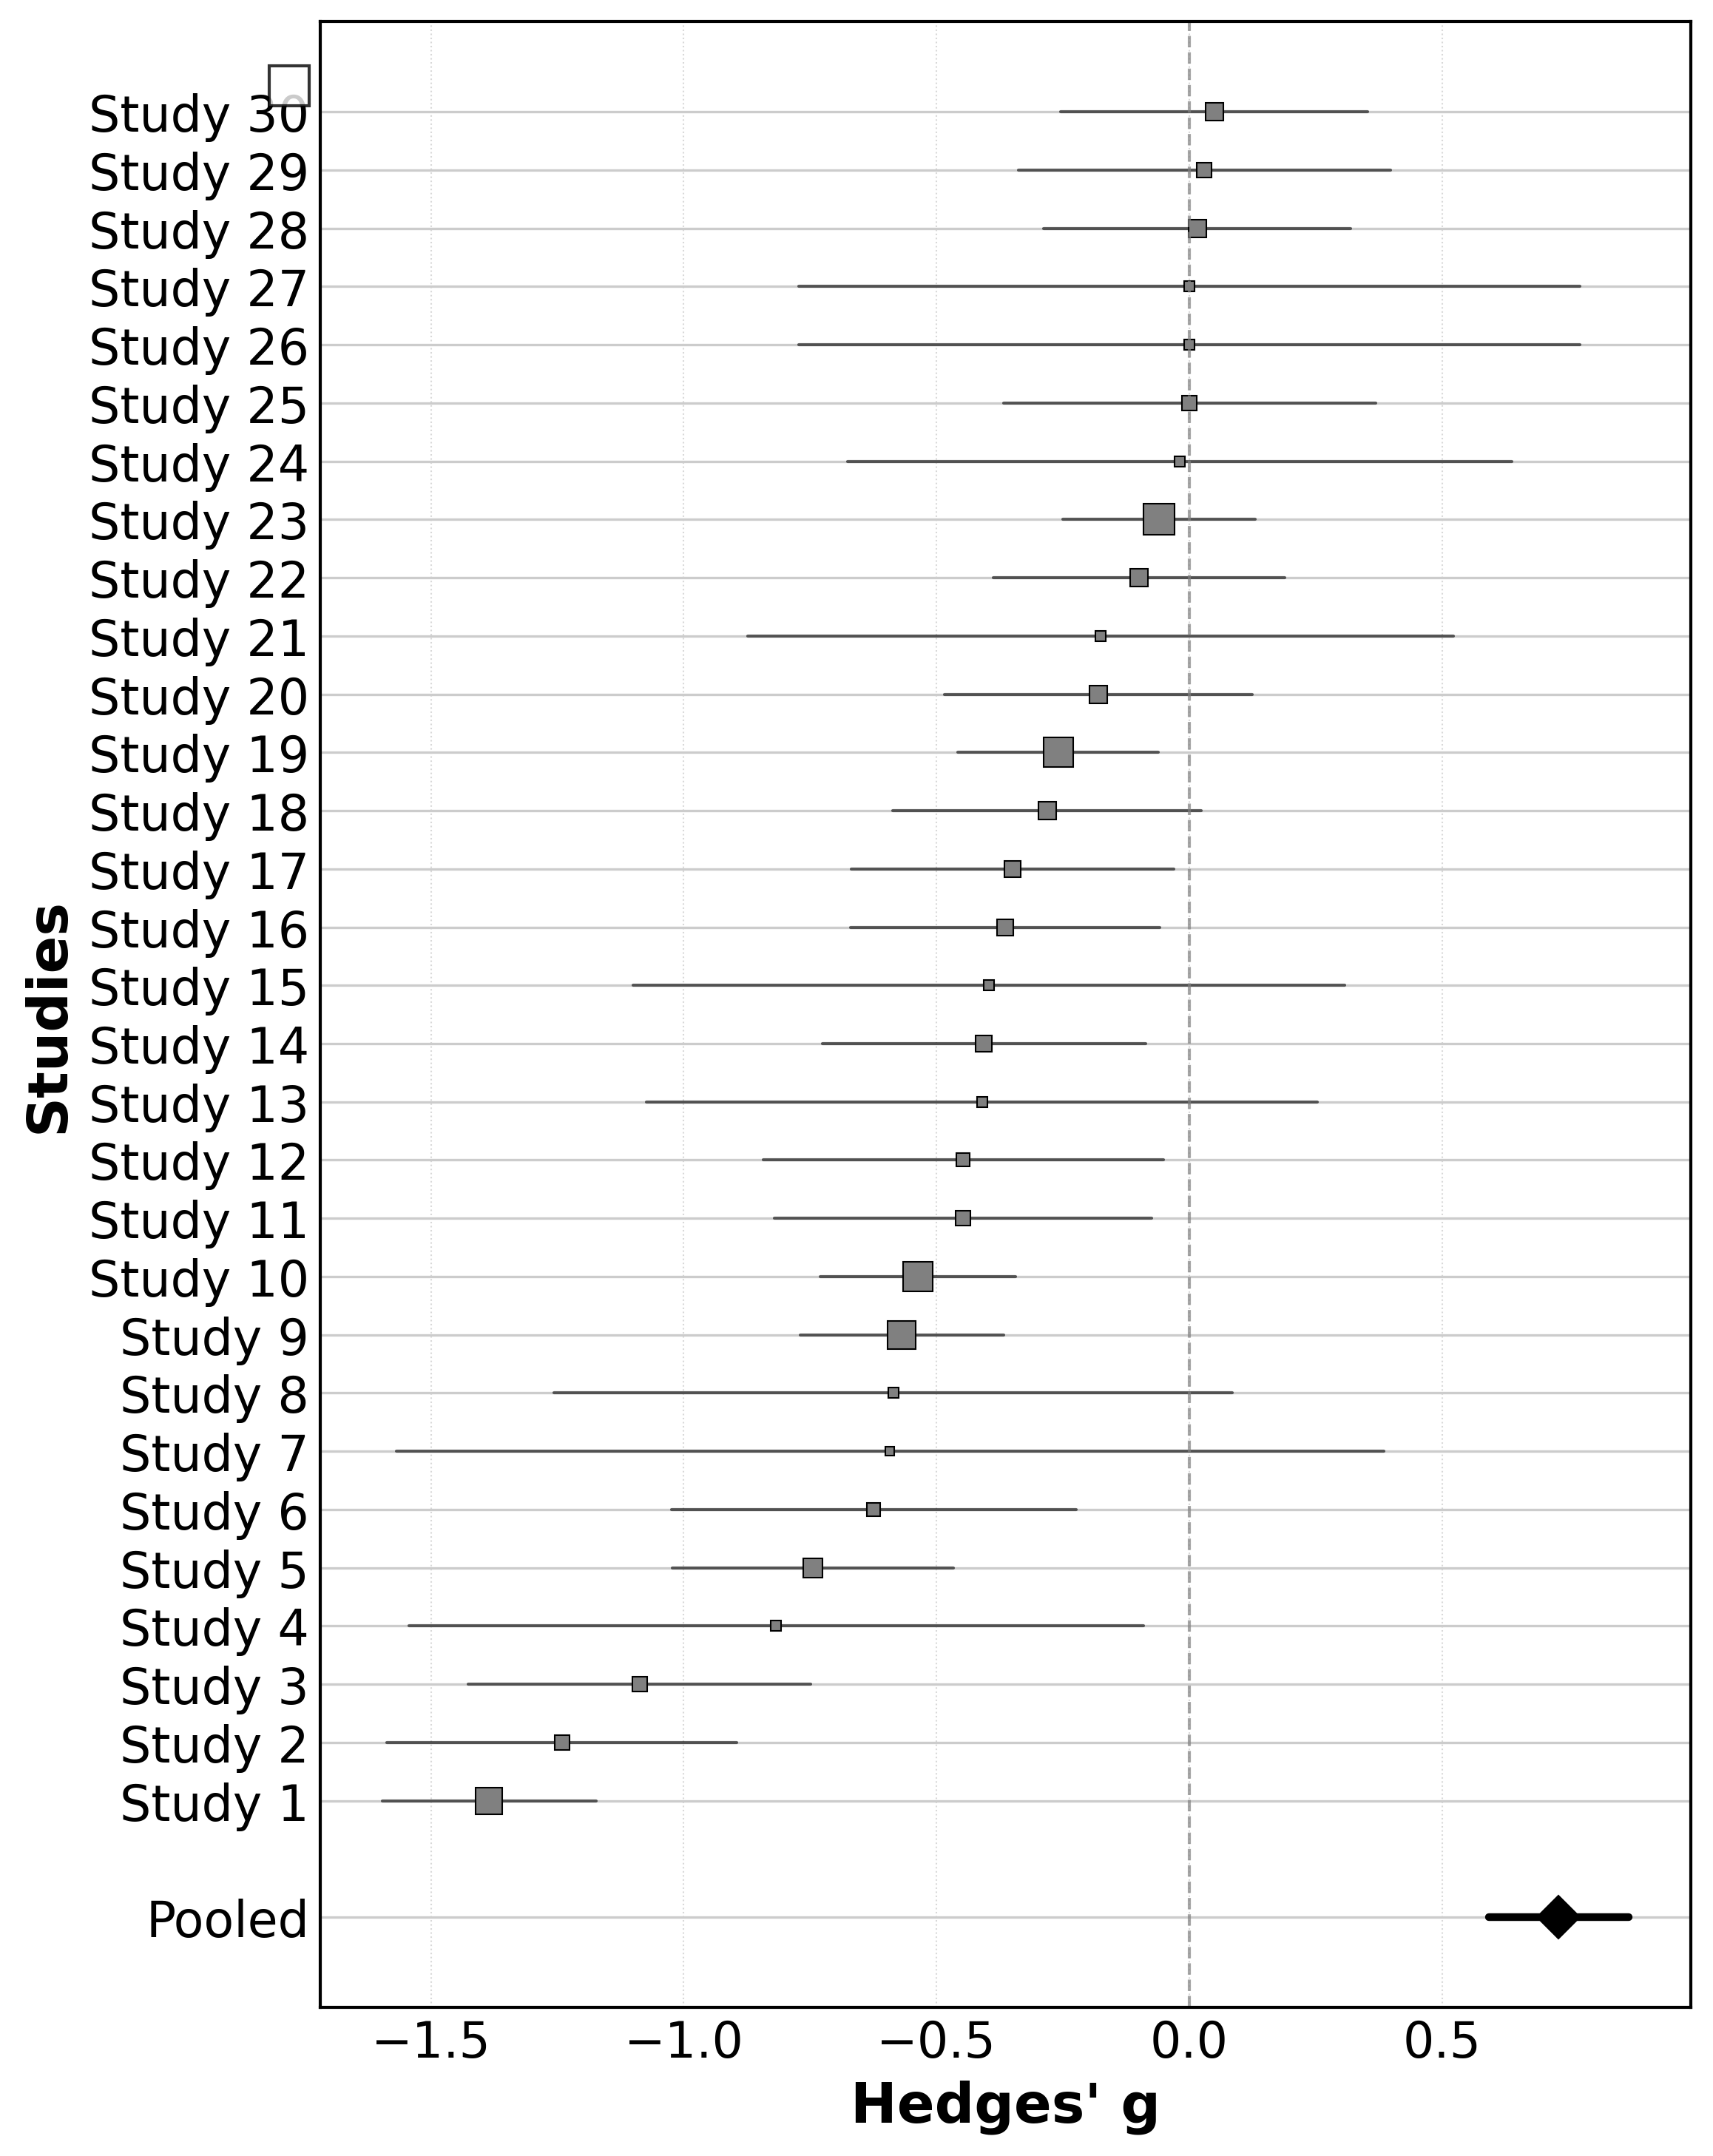
\includegraphics[width=0.4\linewidth]{Figures/figure1_forest_plot (1).png}
%     \caption{Forest plot of the Hedge g values across studies.}
%     \label{fig:forestplot}
% \end{figure}

\subsection{Behavioral and Demographic Attributes} \label{sec:beh}

We found that behavioral attributes created stronger effects than demographic attributes (see Figure \ref{fig:attributes}). Behavioral attributes, including polite versus impolite language, social-oriented versus task-oriented voice feedback, proactive dialogue actions, and repair strategies, indicated substantially stronger effects, $g$ = 0.75, 95\% CI [0.56, 0.93], $k$ = 89, than demographic attributes such as voice, gender (male versus female), assigned demographic identity, visual avatars, and human names, $g$ = 0.69, 95\% CI [0.33, 1.06], $k$ = 42 \footnote{These categories comprise 131 of 169 effects; the remaining 38 examined contextual factors (k = 26) and user moderators (k = 12), analyzed separately.}. Despite the small magnitude difference (8.3\%), this difference was significant, $Q_{\text{between}}$(1) = 151.34, $p$ < .001 ($Q_{\text{within}}$ = 3027.76, $Q_{\text{total}}$ = 3179.09), indicating substantially different heterogeneity patterns between the two categories.

Within behavioral attributes, communication style produced the largest effects, $g$ = 1.16, 95\% CI [0.71, 1.60], $k$ = 25. CAs employing natural conversational patterns, contextually-appropriate formality levels (formal versus informal language), and adaptive politeness strategies (polite versus non-polite phrasing) generated effects approaching one standard deviation. Personality traits produced the second largest effects, $g$ = 1.06, 95\% CI [0.55, 1.59], $k$ = 19, indicating that personality traits (i.e., extraversion, agreeableness, and openness) improve user outcomes. 

Among demographic attributes, visual appearance, $g$ = 0.82, 95\% CI [0.19, 1.45], $k$ = 23, produced stronger effects than demographic identity assignments, $g$ = 0.53, 95\% CI [0.28, 0.77], $k$ = 14. Agents assigned age, gender, or ethnicity outperformed those manipulating only visual elements like avatars or profile pictures. We further analyzed that voice gender (male versus female) showed minimal effects (mean $g$ = 0.26, $k$ = 5), while language status (low-status versus high-status) produced effects (mean $g$ = 1.21, $k$ = 5).

\begin{figure}
    \centering
    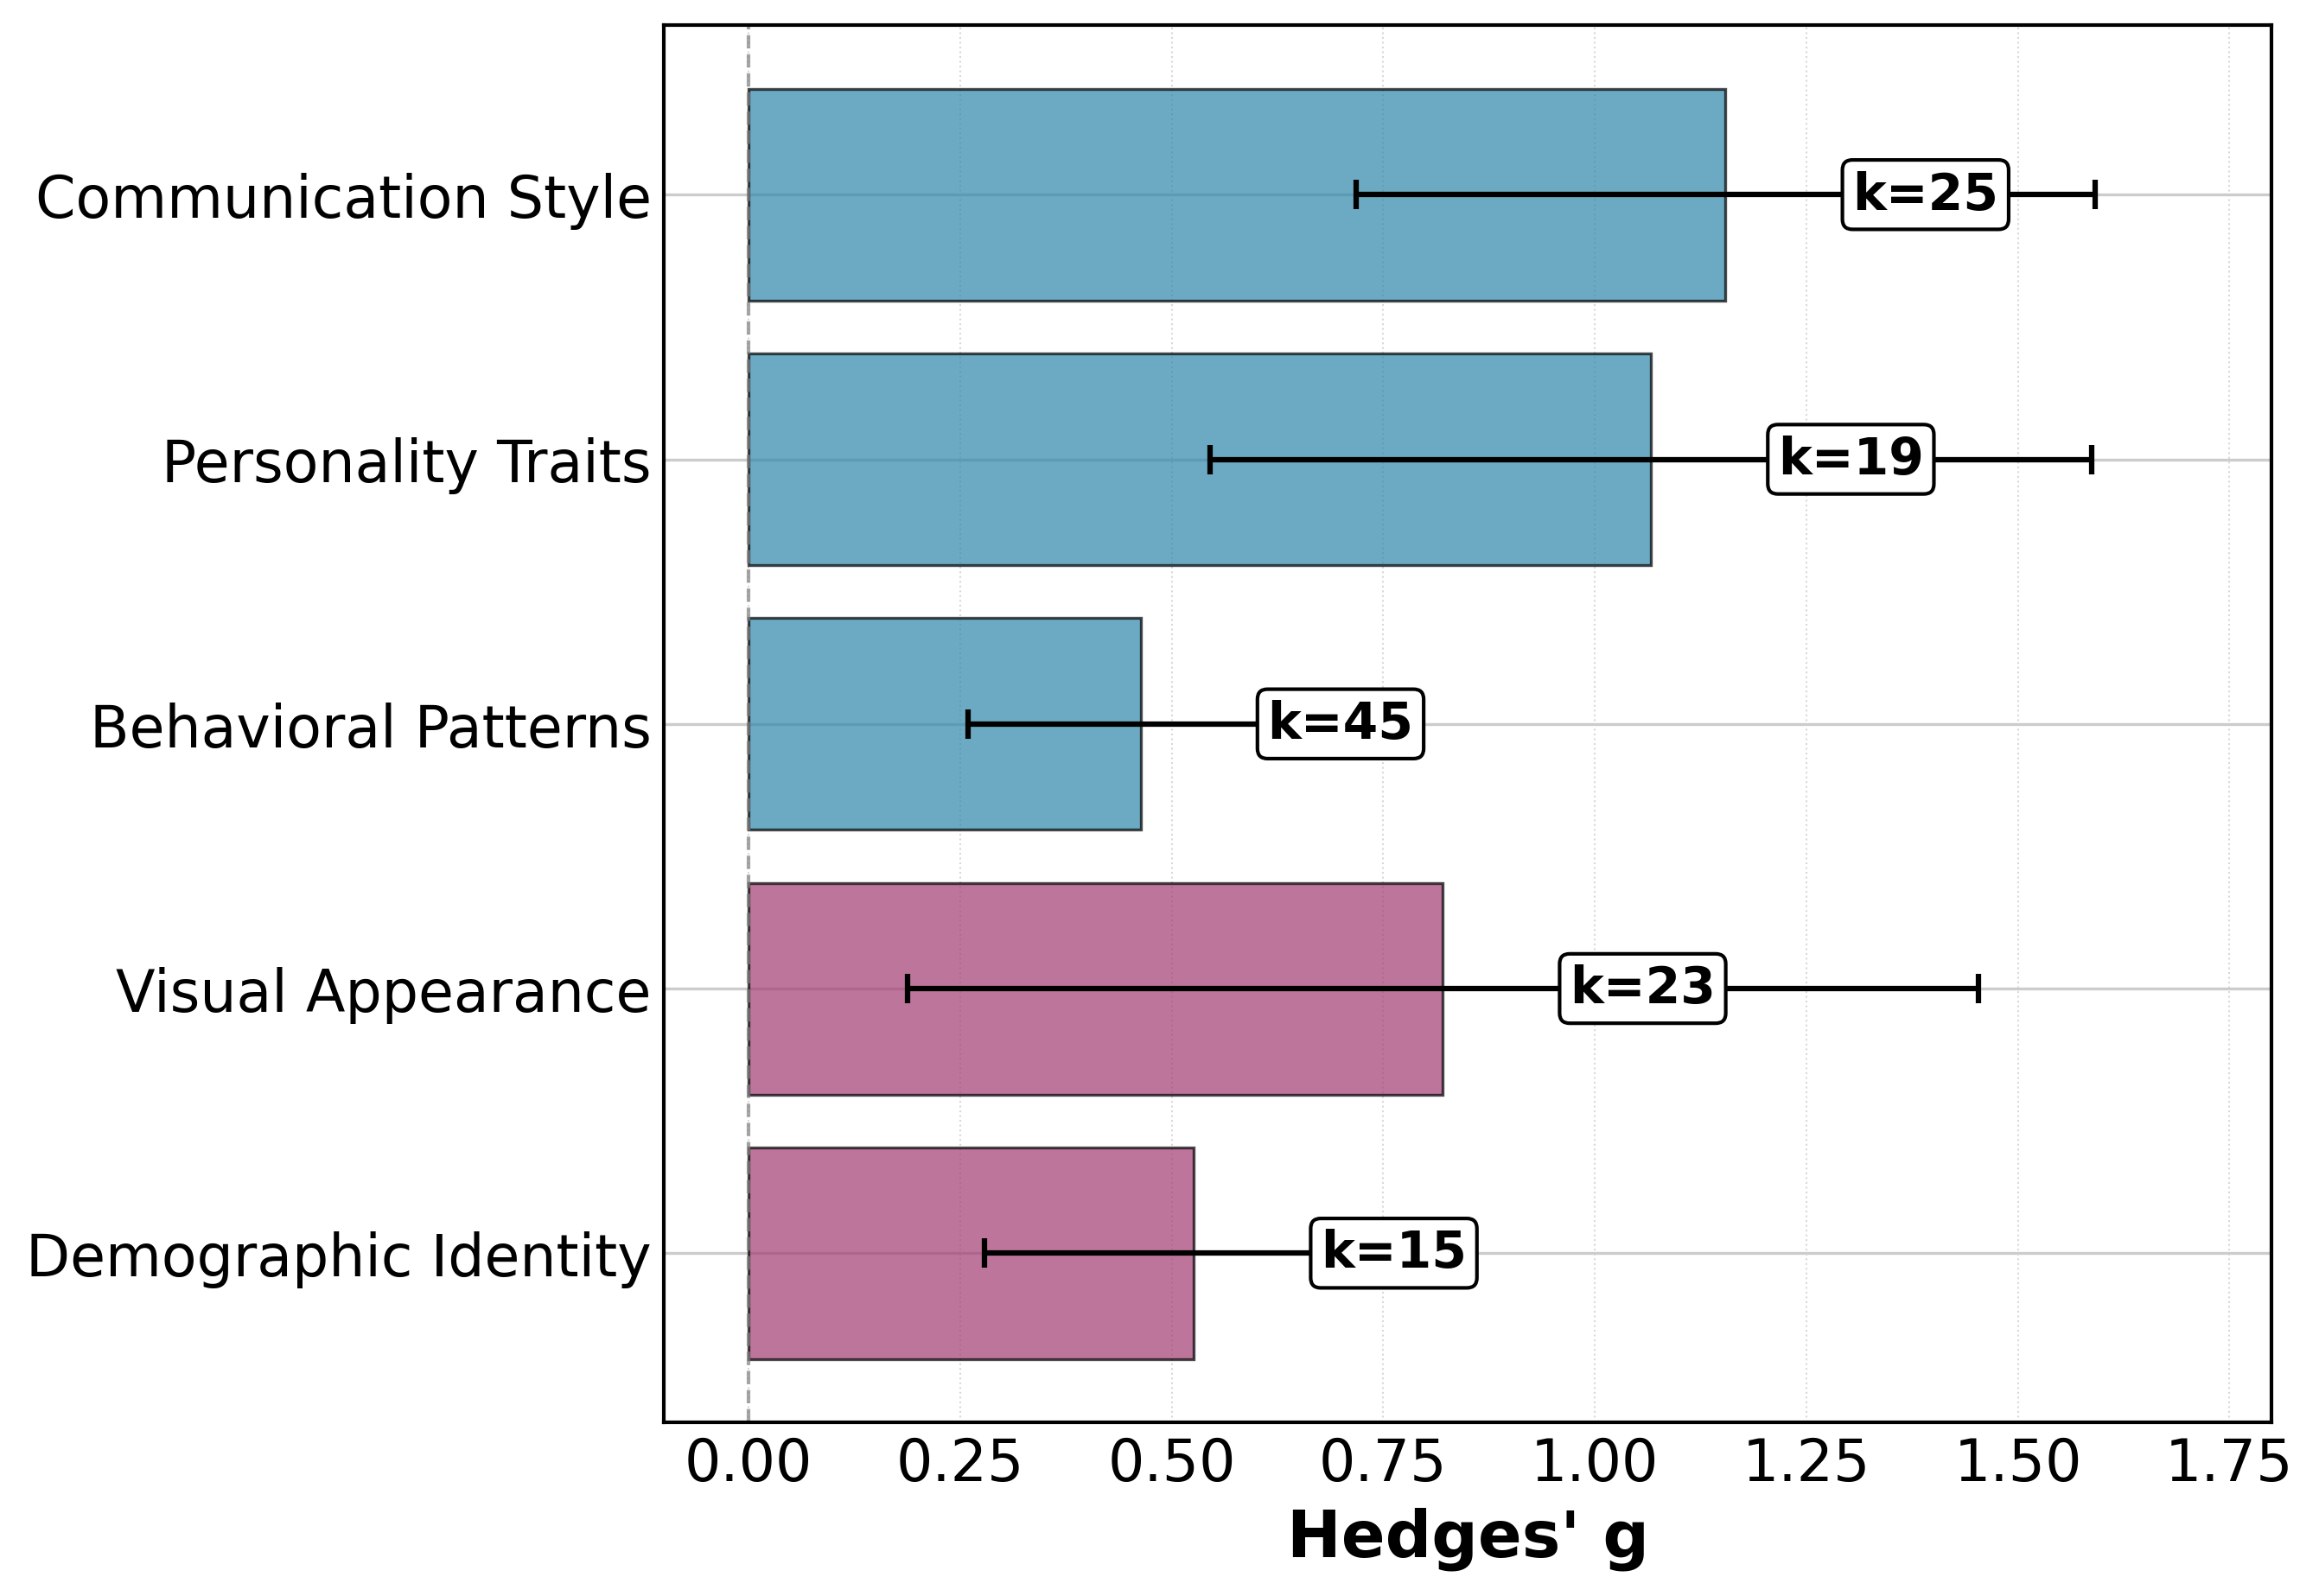
\includegraphics[width=0.5\linewidth]{Figures/figure2a_subcategories.png}
    \caption{Effect sizes for behavioral and demographic attributes for anthropomorphism.}
    \label{fig:attributes}
\end{figure}

\subsection{Effects by Outcome Type} \label{sec:out}

Anthropomorphic attributes affected outcomes differently across measurements. The analysis across the outcome categories showed systematic variation ($Q_{\text{between}}$(6) = 48.23, $p$ < .001), indicating that different attributes have different effect sizes.

UX outcomes showed large effects ($g$ = 0.69, 95\% CI [0.50, 0.88], $k$ = 73). UX outcomes were measured most frequently in research. Perceived usefulness showed moderate to large effects ($g$ = 0.84, 95\% CI [0.28, 1.39], $k$ = 11), while perceived ease of use showed larger effects ($g$ = 1.34, 95\% CI [0.42, 2.26], $k$ = 7). For designers prioritizing user satisfaction and usability, anthropomorphic attributes offer meaningful improvements across multiple experiential dimensions.

Social perception outcomes, measuring perceived humanness, social presence, and relationship quality, showed moderate effects ($g$ = 0.430, 95\% CI [0.143, 0.716], $k$ = 24). Social presence specifically showed the largest effect in the dataset ($g$ = 2.04, 95\% CI [1.00, 3.08], $k$ = 4). These findings indicate that anthropomorphic design most directly influences how human-like and socially present agents appear to users, which aligns with the stated design goals in the reviewed studies.

Trust and credibility outcomes demonstrated moderate-to-large effects ($g$ = 0.66, 95\% CI [0.45, 0.87], $k$ = 24). Trust specifically produced a moderate effect ($g$ = 0.59, 95\% CI [0.20, 0.98], $k$ = 11), while reliability perceptions showed larger effect sizes ($g$ = 0.93, 95\% CI [0.57, 1.29], $k$ = 4). These results suggest that anthropomorphic design can improve user confidence in the system's credibility, addressing concerns about trust establishment in CAs documented in prior research \cite{ng2025trust}.

Learning and performance outcomes showed moderate effects ($g$ = 0.75, 95\% CI [0.16, 1.34], $k$ = 11), with achieved performance demonstrating a large effect ($g$ = 1.00, $k$ = 3). These results suggest that anthropomorphism extends beyond subjective perceptions to influence objective task outcomes, indicating value for educational and task-support applications.

For other outcomes, effects were relatively smaller. Technology acceptance showed small to moderate effects ($g$ = 0.71, 95\% CI [0.17, 1.246], $k$ = 5), while behavioral and interaction patterns showed moderate effects ($g$ = 0.67, 95\% CI [0.31, 1.03], $k$ = 13). This pattern suggests that while anthropomorphism shapes user outcomes, it influences actual usage behaviors more modestly, likely because adoption decisions depend on multiple factors beyond agent design.
Finally, individual differences as moderators showed small effects ($g$ = 1.137, 95\% CI [0.65, 1.623], $k$ = 19), indicating that the effects of anthropomorphism on user outcomes appear relatively consistent between different user populations. %while user characteristics modestly influence anthropomorphic effectiveness, the benefits appear relatively consistent between user populations.

\begin{figure}
    \centering
    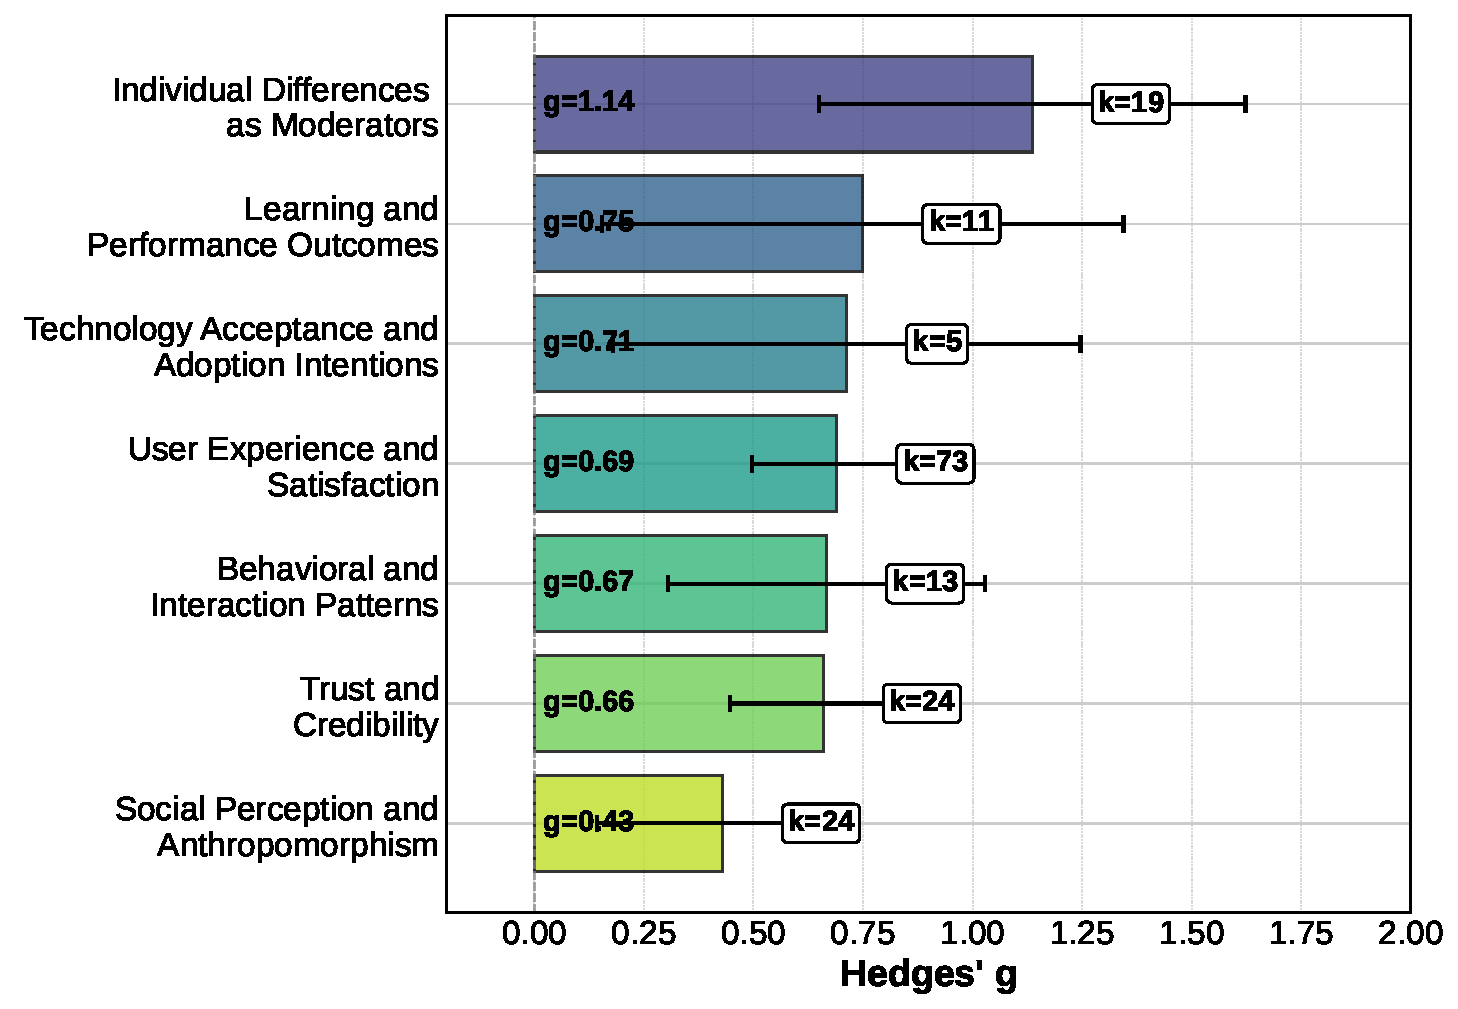
\includegraphics[width=0.5\linewidth]{Figures/figure3_outcome_categories.pdf}
    \caption{User outcomes for the anthropomorphic attributes.}
    \label{fig:outcomes}
\end{figure}

\subsection{Attribute-Outcome Specificity}

While behavioral attributes generally outperform demographic attributes, effect sizes vary substantially across outcomes. We analyzed which anthropomorphic attributes produce the strongest effects for which user outcomes (see Table \ref{tab:meta_matrix}), presented as follows.

\subsubsection{Communication Style Improves UX}\label{sec:comm}

Communication style attributes indicated strong effectiveness for UX outcomes ($g$ = 1.73, 95\% CI [1.11, 2.35], $k$ = 13), nearly double the effect observed for other attribute types. Attributes like politeness calibration, formality adaptation, and natural phrasing produce large effects when measuring satisfaction, usability, and enjoyment. Among the 13 effects in this category, 10 were significant (76.9\%).

For social perception outcomes, communication style again showed large effects ($g$ = 1.30, 95\% CI [0.58, 2.02], $k$ = 6), though with greater variability. Users perceive CAs employing sophisticated communication strategies as more human-like and socially present. However, communication style showed large but unreliable effects on behavioral patterns ($g$ = 1.27, 95\% CI [-0.40, 2.94], $k$ = 3), suggesting that, although users appreciate natural language, it does not consistently influence actual interaction behaviors, such as message frequency or session duration.

\subsubsection{Visual Appearance Shows Outcome-Specific Patterns}

The visual appearance attributes showed a ubiquitous outcome dependence. For trust and credibility, visual attributes produced moderate-to-large effects ($g$ = 0.63, 95\% CI [0.24, 1.02], $k$ = 5), suggesting that professional avatars or appropriate visual design meaningfully influence perceived trustworthiness. However, for UX outcomes, identical visual attributes showed much smaller effects ($g$ = 0.36, 95\% CI [-0.01, 0.73], $k$ = 12), with only 3 of the 12 effects reaching significance (25\%), indicating that visual design alone rarely improves satisfaction or usability.

Unexpectedly, visual appearance showed very large effects when examined as a moderator of other relationships ($g$ = 3.14, 95\% CI [0.59, 5.69], $k$ = 3). This suggests that visual attributes may amplify or attenuate the effects of other attributes instead of exerting strong direct effects themselves, though this interpretation requires caution given the small sample of observed effects in the corpus.

\subsubsection{Demographic identity improves learning outcomes}

Demographic attributes (assigned age, gender, ethnicity, or cultural identity) produced their strongest effects for learning and performance outcomes ($g$ = 0.98, 95\% CI [0.50, 1.46], $k$ = 3), with 2 of 3 effects significant (66.7\%). When CA had relevant demographic attributes, users exhibited better task performance and knowledge acquisition, suggesting that demographic matching or appropriate identity assignment may matter.

For UX, demographic attributes showed moderate effects ($g$ = 0.65, 95\% CI [0.24, 1.06], $k$ = 8), with 3 of 8 effects significant (37.5\%). Users appreciate demographic cues in some contexts but not consistently enough to justify prioritizing them in general-purpose conversational interfaces.

\subsubsection{Actions Work Across Contexts}

Action attributes (including proactivity, repair strategies, and interaction mechanisms) showed consistent moderate effects across diverse outcomes. For learning ($g$ = 0.87, 95\% CI [0.23, 1.52], $k$ = 3), all 3 effects were significant (100\%). For trust ($g$ = 0.30, 95\% CI [-0.10, 0.69], $k$ = 11), all 11 effects were significant (100\%), and for behavioral patterns ($g$ = 0.41, 95\% CI [-0.08, 0.90], $k$ = 7), all 7 effects were significant (100\%). While effect magnitudes remained moderate instead of large, the perfect success rate across all three outcome categories indicates that behavioral attributes, such as appropriate repair strategies, consistently improve user perceptions.

\subsubsection{Personality Traits Show Dual Effectiveness}\label{sec:person}

Personality trait implementations produced moderate-to-large effects for UX ($g$ = 0.62, 95\% CI [0.29, 0.94], $k$ = 10), with 4 of 10 effects significant (40\%). This suggests high variability that may reflect implementation differences, so that consistent personality expression across interactions produces strong effects, while superficial or inconsistent trait displays fail.

% \begin{figure}
%     \centering
%     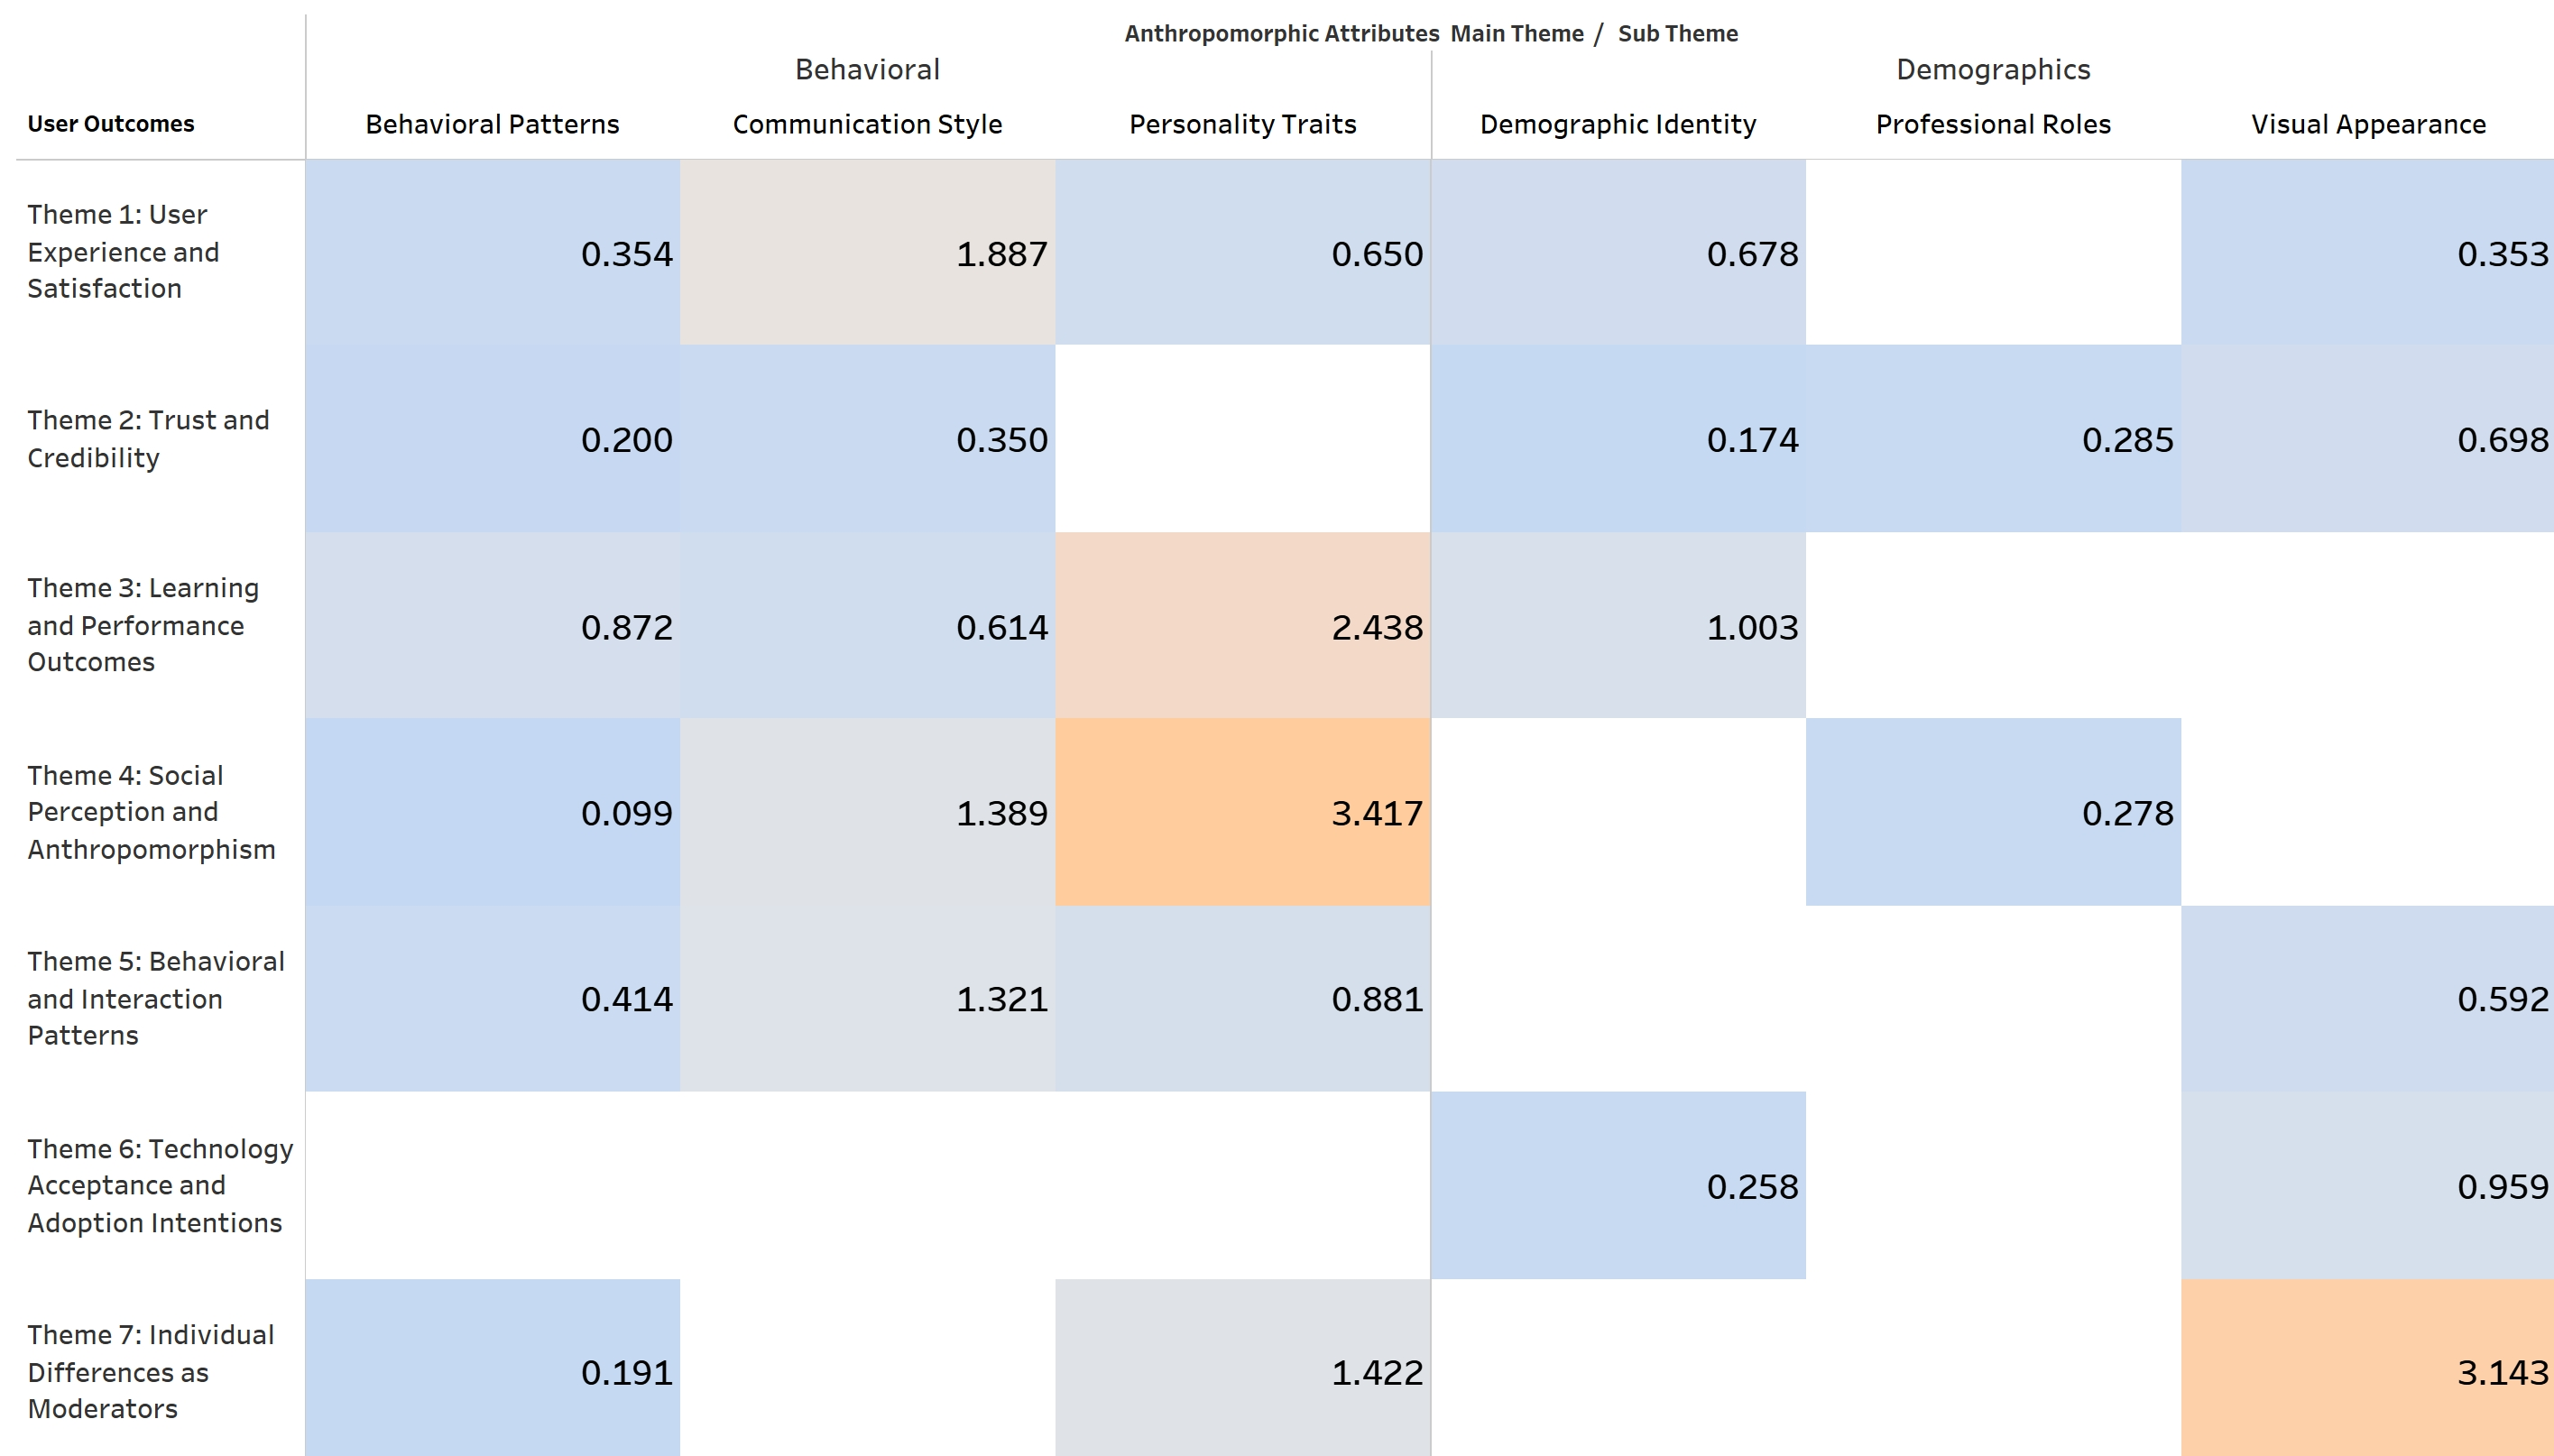
\includegraphics[width=0.8\linewidth]{Figures/heatmap_umap.JPG}
%     \caption{Heatmap correlating the independent variables with dependent variables based on the effect sizes.}
%     \label{fig:ivs_dvs}
% \end{figure}

% Required packages: \usepackage{xcolor,colortbl}, \usepackage{multirow}

% Required packages:
% \usepackage{xcolor,colortbl}
% \usepackage{tabularx}
% \usepackage{array}

% Required packages:
% \usepackage{xcolor,colortbl}
% \usepackage{array}

% Required packages:
% \usepackage{xcolor,colortbl}
% \usepackage{array}

% Column types (put in preamble)
\newcolumntype{L}[1]{>{\raggedright\arraybackslash}p{#1}}
\newcolumntype{C}[1]{>{\centering\arraybackslash}p{#1}}

\begin{table}[htbp]
\centering
\caption{Meta-Analytic Effects of Anthropomorphic Attributes on User Outcomes.
Hedges' \textit{g} values with significance markers (*** \textit{p} < .001, ** \textit{p} < .01, * \textit{p} < .05).}
\label{tab:meta_matrix}
\small
\setlength{\tabcolsep}{2.0pt}
\renewcommand{\arraystretch}{1.0}

\begin{tabular}{L{0.3\columnwidth}|C{0.1\columnwidth}C{0.1\columnwidth}C{0.1\columnwidth}C{0.1\columnwidth}C{0.1\columnwidth}C{0.1\columnwidth}}
\hline
\textbf{Outcome} &
\multicolumn{3}{c}{\textbf{Behavioral}} &
\multicolumn{3}{c}{\textbf{Demographic}} \\
\cline{2-7}
{\small\textbf{}} &
{\small Communi-cation Styles} &
{\small Personality Traits} &
{\small Actions} &
{\small Identity } &
{\small Visual representation} &
{\small Role \& Occupation} \\
\hline

UX and Satisfaction
 & {\cellcolor{green!20}1.73***} & {\cellcolor{yellow!20}0.62***} & {\cellcolor{orange!20}0.35}
 & {\cellcolor{yellow!20}0.65**} & {\cellcolor{orange!20}0.36} & --- \\

Trust and Credibility
 & --- & --- & {\cellcolor{orange!20}0.30}
 & --- & {\cellcolor{yellow!20}0.63**} & --- \\

Learning and Performance Outcomes
 & --- & --- & {\cellcolor{green!20}0.87**}
 & {\cellcolor{green!20}0.98***} & --- & --- \\

Social Perception and Anthropomorphism
 & {\cellcolor{green!20}1.30***} & --- & {\cellcolor{red!20}0.08}
 & --- & --- & {\cellcolor{orange!20}0.28***} \\

Behavioral and Interaction Patterns
 & {\cellcolor{green!20}1.27} & --- & {\cellcolor{orange!20}0.41}
 & --- & --- & --- \\

Individual Differences as Moderators
 & --- & {\cellcolor{green!20}1.40} & {\cellcolor{red!20}0.19}
 & --- & {\cellcolor{green!20}3.14*} & --- \\
\hline
\end{tabular}
\end{table}


\subsection{Triangulation from Multiple Syntheses} \label{sec:triang}

Three complementary synthesis methods validated the quantitative findings using the 373 non-calculable effects. Vote counting showed that 84.2\% of the directional effects were positive, exceeding chance expectation, $p$ < .001 (binomial test). Fisher's combined probability test for 269 effects indicated that the pattern of statistical significance differs from chance, $\chi^2$(2$\times$269) = 1115.85, $p$ < .001. Stouffer's Z-score method indicated predominantly positive effects, $Z(269)$ = 8.84, $p$ < .001. These values (0.025 for significant, 0.50 for non-significant) represent midpoints between typical thresholds and extremes; sensitivity analyses using alternative substitutions (0.01–0.03 for significant, 0.40–0.60 for non-significant) yielded identical conclusions (all $p$ < .001).

All three methods detected significant effects across all seven outcome categories (all $p$-values < .01) and for both the behavioral and demographic attribute types, with behavioral attributes consistently showing stronger evidence. This convergence strengthens confidence that the findings reflect robust patterns rather than artifacts of a single analytical approach.

The analysis of implementation patterns across the 79-article corpus revealed that research practice aligns with the effectiveness findings. Behavioral attributes dominate design choices: communication style appeared in 50.0\% of studies and personality traits in 48.3\%, compared to demographic attributes (37.9\%), assigned roles (24.1\%), and visual appearance (15.5\%). Cohen's $h$ was used to measure the effect size of the difference between two proportions. Overall, behavioral attributes appeared significantly more frequently than demographic attributes (77.6\% versus 41.4\%), $z$ = 3.97, $p$ < .001, Cohen's $h$ = 0.76.

% Specific implementation patterns showed that human names appeared in 37.9\% of studies and strongly predicted gender assignment, $\chi^2$(1) = 15.16, $p$ < .001, Cramer's $\phi$ = .51. Avatars appeared in 36.2\% of studies and associated with voice implementations, $\chi^2$(1) = 3.96, $p$ = .047, Cramer's $\phi$ = .26, suggesting multimodal anthropomorphism strategies. Most studies (72.4\%) employed fixed anthropomorphic attributes, though adaptive implementations increased over time, Spearman's $\rho$ = .83, $p$ = .011. %, potentially signaling evolution toward personalized anthropomorphism.

The publication bias assessment showed mixed findings. Egger's regression test detected significant asymmetry (intercept = 2.21, $SE$ = 0.71, $t$(167) = 3.11, $p$ = .002), indicating smaller studies reported larger effects. However, the fail-safe $N$ analysis showed 620 unpublished null studies would be needed to nullify the results, exceeding Rosenthal's criterion \cite{rosenthal1979file} of 125 ($5\times23+10$) by a factor of 4.96, suggesting robustness despite potential small-study bias. However, as the Egger's test is considered to be more accurate of the two, we confirm the results with funnel plots (see online appendix for details) and confirm that a publication bias is evident in the corpus.

Our synthesis of 542 effects from 79 studies indicates that anthropomorphic attributes consistently produce positive effects, $g$ = 0.73, with effectiveness depending on how these are implemented. Behavioral attributes ($g$ = 0.75), particularly communication style ($g$ = 1.16), personality traits ($g$ = 1.06), and responsiveness ($g$ = 0.69), consistently improve outcomes more than demographic attributes ($g$ = 0.69). The effects are most pronounced on learning ($g$ = 0.75) and UX ($g$ = 0.69), with moderate effects on behavioral outcomes ($g$ = 0.67) and trust ($g$ = 0.66), and smaller effects on social perception ($g$ = 0.43). The results from all synthesis methods are consistent with these conclusions. %, strengthening confidence in the findings.

\section{Discussion}

%This meta-analysis synthesized 583 effects from 79 studies examining anthropomorphism in CAs. Our findings reveal that anthropomorphic design consistently enhances user outcomes, with critical asymmetries between behavioral and demographic design. We interpret these patterns through theoretical lenses, derive specific practical guidelines, and identify limitations that bound our conclusions.

\subsection{Theoretical Implications}

%\textit{Theoretical Implications: }
This study contributes to CA anthropomorphism research by identifying which specific attributes matter most, for which outcomes, and to what degree. Specifically our findings lend support for the CASA theory \citep{nass1997machines}, which proposes that social cues in computer interfaces trigger social responses. Both behavioral and demographic anthropomorphic attributes produced positive effects, with behavioral attributes showing slightly stronger effects. This pattern aligns with CASA's prediction that social cues influence user responses, though the magnitude difference between attribute types was modest.

Within these categories, we observed heterogeneity in effectiveness. Communication style showed stronger effects than other behavioral attributes, while visual appearance outperformed demographic identity assignments among demographic attributes. These differences indicate that implementation choices within anthropomorphic design influence outcomes. The heterogeneity in the effectiveness of anthropomorphism should be further studied. Possible variables that we did not analyze include implementation quality, context, and user demographics.

Our contribution here is quantifying these effects and identifying which specific anthropomorphic attributes produce the strongest outcomes. Communication style and personality expression emerge as particularly effective design choices. The meta-analytic approach identifies which anthropomorphic attributes produce stronger outcomes in existing research. Communication style and personality traits showed larger effect sizes than demographic assignments in our corpus. This suggests that CA's communication design (tone, word choice, personality expression) warrants more attention than what demographic attributes, these agents belong to. We may want to place greater emphasis on  ``how the agent continuously acts'' instead of on ``what the agent appears to be.''

Our results relate to Klein's \cite{klein_effects_2025} meta-analysis of text-based CAs with some differences. Our overall effect is larger, potentially because our corpus includes voice-based and multimodal CAs in which behavioral attributes such as prosody and timing extend beyond text. Our behavioral and demographic categorization provides an alternative way to analyze human-like social cues, showing that implementation type affects outcomes within anthropomorphic design. Also, Klein's text-only scope excluded voice-based attributes that showed significant effects in our analysis. Klein's work indicates that anthropomorphism improves user outcomes \citep{klein_effects_2025}, while our study extends this finding across modalities.

\subsection{Practical Implications: }
In terms of practical implications, based on our findings, we propose \change{five} design guidelines (DGs) for anthropomorphism in CAs:

\textbf{DG1: Prioritize communication style over visual design} (Section \ref{sec:beh}). \change{Invest development resources in natural language generation, formality adaptation, and politeness strategies rather than avatar selection or demographic assignment. Behavioral personalization i.e. adapting communication style and personality expression to user preferences, consistently outperforms demographic-based personalization such as matching agent gender or ethnicity to the user.}
\textbf{DG2: Implement coherent personality} (Section \ref{sec:person}). \change{Express personality through consistent behavioral patterns rather than static declarations. An agreeable CA, for example, should prioritize cooperative phrasing across every response; an extroverted CA should consistently initiate and sustain engagement. In contrast, an inconsistent personality expression tend to the social contract and creates confusion.}

\textbf{DG3: Build proactive responsiveness} (Section \ref{sec:beh}). CA developers should implement adaptive behaviors, including proactive dialogue actions, intelligent turn-taking, and effective repair strategies. Ideally, the CA anticipates user needs without seeming intrusive, and responds appropriately when misunderstandings occur (i.e., suggestion versus rephrase strategy).

\textbf{DG4: Match anthropomorphic attributes with outcomes} (Section \ref{sec:out}). \change{Attribute selection should follow the intended outcome. For example, communication style attributes produce their largest effects on UX (g = 1.73) and social perception (g = 1.30), making them the priority for companionship or service interfaces. Similarly demographic identity attributes produce their strongest effects on learning performance (g = 0.98), making them relevant primarily for educational or tutoring contexts.}

% \textbf{DG5: Anthropomorphize behavior, not demographics} (Section \ref{sec:beh}). CA developers should tailor the CA's communication style to user preferences (formal versus informal, verbose versus concise) and personality expression to user traits instead of matching demographic characteristics. Behavioral personalization outperforms demographic-based personalization.

\textbf{DG5: Manage expectations for behavioral outcomes} (Section \ref{sec:out}). \change{Anthropomorphism improves perceptions substantially but shows modest effects on adoption intentions (g = 0.71) and behavioral patterns (g = 0.67). A CA that communicates warmly but fails at core tasks will not overcome adoption barriers through persona alone. Developers are encouraged to treat anthropomorphic design as a complement to functional quality, and set realistic expectations internally when communicating its impact to stakeholders.}

\subsection{Limitations and Future Directions}
%\textit{Limitations and Future Directions: }
When interpreting our findings, some limitations should be considered. First, multiple dependent effects per study (M = 7.3) likely underestimate standard errors because treating non-independent observations as independent artificially increases precision, making confidence intervals too narrow and p-values too small. Sensitivity analysis aggregating to one effect per study yielded consistent but smaller effects ($g$ = 0.54 vs. 0.73), suggesting the primary estimate may be somewhat inflated. 

Future meta-analyses should employ multilevel models \cite{vandennoortgate2013} to examine the differential moderator-level effects. \change{Moreover, whether behavioral and demographic attributes interact, for instance, whether communication style effects are amplified when paired with a coherent demographic identity, remains an open question. The current dataset does not contain sufficient effects examining these combinations to permit subgroup analysis, but this represents a productive direction for future meta-analytic work as the literature matures.}

Second, Egger's test detected significant funnel plot asymmetry ($p$ = .002), indicating small studies reported larger effects. This could reflect publication bias or genuine methodological differences between small and large studies. The large fail-safe $N$ (n = 620) suggests that the findings remain robust despite this asymmetry, although the effect magnitude estimates should be interpreted cautiously especially as Egger's metric shows the potential for larger publication bias. Third, substantial heterogeneity ($I^2$ = 95.4\%) and a wide prediction interval [-0.97, 2.43] indicate considerable variation across studies, with some CA implementations producing negative effects. 

In addition to addressing these limitations, future research could investigate how moderators such as implementation quality, interaction duration, task characteristics, and cultural context influence the variability of effects and identify boundary conditions for CAs' anthropomorphic design. We make our coding sheet available for others to build on\footnote{\href{https://osf.io/7rj6f/overview?view_only=35b327583fee4222b5b336465107580c}{https://osf.io/7rj6f/overview?view\_only=35b327583fee4222b5b336465107580c}}.

\change{Lastly, while our corpus spans both pre-LLM and LLM-based studies, which raises the question of whether effect sizes differ systematically between these periods. The available data do not permit a clean subgroup analysis on this dimension, as study reporting rarely specifies whether the underlying CA uses an LLM explicitly. Future meta-analyses covering this period should code LLM use as a categorical moderator, given that LLM-based CAs may produce qualitatively different anthropomorphic effects through their superior language fluency and contextual adaptation compared to rule-based predecessors.}

\subsection{Ethical Considerations of Anthropomorphic Design in CAs}
\change{The anthropomorphic design of CAs raises ethical concerns that practitioners must address. Human-like communication can produce parasocial dependency, where users form emotional attachments to agents incapable of genuine reciprocation, a risk that has already been raised and needs further imploration \citep{laura_kuenssberg_mothers_2025}. Anthropomorphism can also lower users' critical evaluation of CA outputs, functioning as an inadvertent manipulation mechanism \citep{chaves2021should}. Beyond individual harms, demographic attribute assignments risk encoding and reinforcing social stereotypes, particularly when gender or ethnicity are paired with specific occupational roles. Designers should therefore treat persona consistency and disclosure of artificial identity as ethical obligations in all deployment contexts.} %, not optional design decisions.}
% \section{Results}

% \subsection{Corpus Overview}

% The final corpus included 79 articles published 2018-2025 (Figure~\ref{fig:prisma}). The publication frequency was 7 articles during 2018-2020, 14 articles in 2021, 12 articles in 2022, 14 articles in 2023, and 32 articles in 2024.
% Most articles were research articles (n = 76, 96.2\%), with remaining articles comprising reviews, case articles, and perspective pieces (n = 3, 3.8\%). Quality assessment showed 81.0\% (n = 64) were published in JUFO-ranked venues: 44 articles (55.7\%) in level 1 venues, 9 articles (11.4\%) in level 2, and 11 articles (13.9\%) in top-tier level 3 venues.
% The corpus has a strong empirical focus: 75 articles (94.9\%) conducted primary data collection, with only 4 articles (5.1\%) taking conceptual approaches. Notably, 65 articles (82.3\%) included human participant experiments. Research was carried out in different fields, though specific field distributions require analysis of the 58 articles that implemented anthropomorphization attributes.

% \subsection{Theme 1: User Experience and Satisfaction}

% This theme encompasses the largest cluster of findings, examining how users perceive their overall experience with conversational user interfaces. The dependent variables within this theme include overall satisfaction, enjoyment, usability scores (measured via SUS, UEQ, UEQ-S, SASSI), attractiveness, pragmatic qualities, hedonic qualities, pleasantness, and ease of use.

% \subsubsection{Overall Usability Assessments}

% Several studies employed standardized usability instruments to evaluate conversational interfaces, with generally positive results across diverse application domains. The character-based COVID-19 chatbot Chasey achieved notably high usability with a mean SUS score of 89.3 ($SD = 8.69$), substantially exceeding the standard acceptability threshold of 68 and qualifying for an ``A'' grade \cite{A79}. Similarly, the Wordbot medical terminology learning system demonstrated strong usability with a mean SUS score of 83.25 ($SD = 5.22$), also surpassing the threshold for ``good'' usability \cite{A34}. The AI-driven VTuber system KawAIi achieved CUQ scores significantly exceeding the 68-point acceptability threshold, indicating strong usability across personality, onboarding, user experience, and error handling dimensions \cite{A81}.

% These findings suggest that well-designed conversational interfaces can achieve high usability ratings regardless of their specific domain application, whether healthcare information provision, educational vocabulary training, or entertainment-oriented virtual streaming.

% \subsubsection{Multidimensional User Experience Evaluations}

% Studies employing multidimensional UX instruments revealed nuanced patterns across pragmatic and hedonic quality dimensions. The NewtBot physics tutoring system demonstrated positive user experience across all three interaction modes (Baseline, Tutor, Feedback), with all conditions achieving significantly positive mean UEQ-S scores above the neutral threshold \cite{A22}. The Tutor mode achieved the highest overall UEQ-S score ($M = 0.985$, $SD = 0.439$), followed by Feedback ($M = 0.847$, $SD = 0.467$) and Baseline ($M = 0.767$, $SD = 0.648$) \cite{A22}. Notably, all groups scored above 0.8 on pragmatic quality subscales indicating positive functional evaluation, while hedonic quality ratings fell within the neutral range (between $-0.8$ and $0.8$), suggesting that while the system was perceived as functionally effective, it was not particularly stimulating or novel \cite{A22}.

% Research examining proactive dialogue actions in conversational agents found that notification-based proactive behaviors yielded superior user experience compared to more intrusive intervention strategies. Specifically, notification actions received significantly higher UEQ ratings for both attractiveness and hedonic quality compared to intervention and suggestion actions \cite{A16}. This pattern suggests that users prefer conversational agents that inform instead of interrupt or override user autonomy.

% Investigation of visual embodiment in smart display voice assistants revealed no significant differences in UX ratings across disembodied (DEA), artificially rendered (AEA), and photorealistic (PEA) agent conditions \cite{A86}. All three conditions achieved comparably positive ratings on both UEQ and AttrakDiff instruments, with high pragmatic quality scores (UEQ Pragmatic: DEA $M = 1.67$, AEA $M = 1.43$, PEA $M = 1.71$) and moderate hedonic quality scores (UEQ Hedonic: DEA $M = 0.84$, AEA $M = 0.81$, PEA $M = 0.99$) \cite{A86}. This null finding indicates that adding visual embodiment neither significantly improves nor diminishes measured user experience in task-oriented contexts, opening design space for embodiment decisions based on considerations beyond UX metrics.

% \subsubsection{Satisfaction and Enjoyment}

% Direct assessments of user satisfaction revealed generally positive responses to conversational interfaces across contexts. Users of a recidivism risk assessment chatbot reported moderate-to-high satisfaction, with 64.3\% indicating they were ``satisfied'' or ``very satisfied'' with the overall experience ($M = 3.63$, $SD = 0.82$ on a 5-point scale) \cite{A54}. Notably, enjoyment ratings were even higher, with 78.5\% reporting satisfaction with how much they enjoyed using the chatbot ($M = 3.91$, $SD = 0.80$) \cite{A54}. This pattern of enjoyment exceeding general satisfaction suggests that conversational interfaces may provide intrinsic value beyond their functional utility.

% The COVID-19 chatbot Chasey achieved high satisfaction ratings on semantic differential scales, with an overall satisfaction score of $M = 1.45$ ($SD = 0.56$) on a scale ranging from $-2$ to $+2$ \cite{A79}. Users rated the experience as pleasant ($M = 1.56$), good ($M = 1.61$), nice ($M = 1.50$), and likeable ($M = 1.33$), consistently selecting positive over negative descriptors \cite{A79}. The KawAIi VTuber system similarly received positive pleasantness ratings, with users judging the interaction experience favorably and finding conversations enjoyable and rewarding \cite{A81}.

% \subsubsection{Pragmatic Qualities: Usefulness, Ease of Use, and Efficiency}

% Perceived usefulness emerged as a consistent strength across conversational interface evaluations. The recidivism chatbot received high usefulness ratings, with 76.8\% of users indicating satisfaction with its utility for assessing recidivism risk ($M = 3.97$, $SD = 0.81$) \cite{A54}. The COVID-19 chatbot achieved an aggregate usefulness score of $M = 1.5$ ($SD = 0.48$) on a $-2$ to $+2$ scale, with users strongly endorsing descriptors such as ``assisting'' ($M = 1.69$), ``useful'' ($M = 1.56$), and ``effective'' ($M = 1.33$) \cite{A79}. The majority of NewtBot users agreed that the system helped them complete tasks more quickly, supporting perceived efficiency gains from conversational tutoring \cite{A22}.

% Ease of use ratings were generally positive but showed more variability. The recidivism chatbot achieved 70.5\% satisfaction for ease of use ($M = 3.70$, $SD = 0.79$) \cite{A54}, while the Chasey chatbot's highest-rated SUS item was ``easy to use'' ($M = 4.81$, $SD = 0.47$) with corresponding low ratings for ``unnecessarily complex'' ($M = 1.31$, $SD = 0.52$) indicating a non-complex system \cite{A79}.

% However, specific usability challenges emerged in certain contexts. The recidivism chatbot showed weakness in answer understandability, with only 57.1\% expressing satisfaction and 22.3\% indicating dissatisfaction ($M = 3.42$, $SD = 0.95$), making this the lowest-rated usability dimension \cite{A54}. Time acceptability also showed mixed results, with 56.2\% satisfied but 28.6\% dissatisfied ($M = 3.46$, $SD = 1.24$), exhibiting the highest standard deviation among usability items and suggesting substantial individual variation in temporal expectations \cite{A54}.

% \subsubsection{Interface Type and Modality Effects}

% Research examining interface modality variations produced predominantly null findings for user experience outcomes. Investigation of baseline, speech-only, and hybrid conversational interfaces found no significant effects on perceived ease of use, usefulness, or UEQ-S ratings for either pragmatic or hedonic qualities \cite{A15}. Similarly, TAM-based measures of perceived usefulness and perceived ease of use showed no significant differentiation across interface types \cite{A15}. These findings suggest that the addition of speech modality or hybrid interaction capabilities may not substantially alter user experience perceptions in isolation.

% The equivalence of visual embodiment conditions (disembodied, artificial, photorealistic) on UX measures similarly indicates that agent visualization does not automatically confer experience benefits \cite{A86}. All three embodiment conditions were classified as ``task-oriented'' by AttrakDiff, exhibiting high pragmatic and medium hedonic profiles typical of functional tools \cite{A86}. The convergence of two independent validated instruments (UEQ and AttrakDiff) on this null finding strengthens confidence in the conclusion that embodiment decisions can be made on grounds other than quantitative UX impact.

% \subsubsection{Repair Strategies and Conversational Design}

% Conversational repair strategies demonstrated differential effects on user experience dimensions. The use of suggestion-based repair strategies (offering alternative phrasings when misunderstandings occur) led to significantly higher perceived accuracy and likability compared to rephrase-based strategies \cite{A13}. However, repair strategy type showed no significant effect on other SASSI-measured dimensions \cite{A13}. Politeness manipulations (polite versus non-polite agent responses) produced no main effects on user experience measures, though an interaction effect emerged wherein the effectiveness of politeness depended on the accompanying repair strategy type \cite{A13}.

% \subsubsection{attribute-Specific Evaluations}

% When users evaluated specific attributes within conversational systems, differential preferences emerged. Among COVID-19 chatbot attributes, FAQs received the highest ratings ($M = 4.83$, $SD = 0.45$), followed by Cases Tracker ($M = 4.72$, $SD = 0.51$), WHO Advice ($M = 4.61$, $SD = 0.60$), and Screening/Symptoms Checker ($M = 4.56$, $SD = 0.77$) \cite{A79}. Despite the symptoms checker receiving the lowest rating, all attributes scored highly (above 4.5 on a 5-point scale), leading to the recommendation that chatbots should incorporate multiple attribute types instead of focusing solely on symptom checking functionality \cite{A79}.

% \subsubsection{Summary of Theme 1 Findings}

% The evidence across this theme indicates that conversational user interfaces can achieve high usability and satisfaction ratings across diverse application domains including healthcare, education, entertainment, and professional training. Standardized usability scores consistently exceeded acceptability thresholds, and users generally reported positive satisfaction and enjoyment. Pragmatic qualities (usefulness, efficiency, ease of use) emerged as particular strengths, while hedonic qualities (stimulation, novelty) showed more moderate ratings, suggesting that current CUI implementations excel at functional utility but may not consistently provide exciting or innovative experiences.

% Interface modality variations and visual embodiment manipulations produced largely null effects on quantitative UX measures, indicating that these design decisions can be made based on considerations beyond UX scores without risking experience degradation. Conversational repair strategies showed selective effects, with suggestion-based approaches enhancing perceived accuracy and likability. attribute diversity within chatbots appears valued by users, with multiple information-provision options preferred over single-purpose designs.

% Notable variability emerged in user perceptions of answer understandability and interaction time requirements, highlighting ongoing challenges in conversational interface design that warrant attention in future development efforts.

% \subsection{Theme 2: Trust and Credibility}

% This theme examines user perceptions of trustworthiness, reliability, and credibility in conversational user interfaces. Trust represents a critical factor in CUI adoption and continued use, particularly in high-stakes domains such as healthcare, professional training, and decision support. The dependent variables within this theme include general trust ratings, perceived reliability, technical competence, understandability, faith, credibility, benevolence, and perceived question understanding.

% \subsubsection{Proactive Dialogue Actions and Trust Dimensions}

% Research examining proactive dialogue behaviors in conversational agents revealed nuanced effects across multiple trust dimensions. The study investigating four proactive action types (None, Notification, Suggestion, Intervention) found that notification-based actions consistently outperformed more intrusive intervention strategies across trust subscales derived from Madsen and Gregor's trust model \cite{A16}.

% For perceived technical competence, notification actions received significantly higher ratings than no-action and intervention conditions for easier tasks, while notification was rated higher than intervention for more challenging tasks \cite{A16}. This pattern suggests that proactive information provision enhances perceptions of system capability, whereas autonomous intervention may undermine confidence in system competence.

% Perceived understandability showed a similar pattern, with notification actions rated higher than no-action conditions for easier tasks, and both notification and no-action conditions rated higher than intervention for harder tasks \cite{A16}. The finding that intervention reduced perceived understandability even compared to no proactive action indicates that autonomous system behaviors may create confusion about system functioning and decision-making processes.

% Reliability perceptions favored notification actions, which received significantly higher ratings than both intervention and no-action conditions \cite{A16}. Faith in the system likewise showed notification superiority over intervention \cite{A16}. These consistent patterns across trust dimensions establish notification as the optimal proactive dialogue strategy for building user trust, while intervention-based approaches appear counterproductive despite potentially offering greater assistance.

% \subsubsection{Trust Development Over Time}

% Longitudinal trust dynamics revealed important patterns in how trust evolves through interaction experience. Initial trust levels, measured before task engagement, showed subsequent increases following system use, though the magnitude and timing of trust gains varied by proactive action condition \cite{A16}.

% For notification-action conditions, trust increased significantly from initial measurement to completion of the first task \cite{A16}. Suggestion-action conditions showed the same pattern of trust increase from initial to post-first-task measurement \cite{A16}. In contrast, no-action conditions demonstrated trust increases occurring later, specifically from the first task to the second task instead of from initial exposure \cite{A16}. These differential trajectories suggest that proactive behaviors (notification and suggestion) accelerate trust calibration, enabling users to form confident trust judgments more quickly, while passive systems require extended interaction for trust development.

% \subsubsection{Gender Differences in Trust Perceptions}

% Gender emerged as a moderating factor in trust responses to proactive dialogue actions. Female users showed significant differences in perceived technical competence and reliability ratings, with notification actions rated higher than no-action conditions during the first task \cite{A16}. For the second task, female users rated both no-action and notification conditions higher than intervention for understandability \cite{A16}. Faith ratings also showed significant condition differences specifically for female users \cite{A16}.

% These gender-specific effects suggest that female users may be more sensitive to proactive dialogue design choices, exhibiting stronger differentiation between action types. The finding has implications for inclusive design, indicating that dialogue strategies optimized for general populations may not equally serve all user groups.

% \subsubsection{Interface Modality and Trust}

% Investigation of interface modality effects (baseline, speech-only, hybrid) on trust produced predominantly null findings. Neither the Trust Scale by Jian, Bisantz, and Drury nor reverse-scored distrust measures showed significant differences across interface conditions \cite{A15}. A trend toward higher trust in hybrid CUI conditions emerged, but post-hoc analysis revealed no significant pairwise differences between conditions \cite{A15}.

% This null finding indicates that the addition of speech modality or hybrid interaction capabilities does not inherently enhance trust perceptions. Trust appears to be driven by factors beyond interface modality, suggesting that conversational designers cannot rely on modality choices alone to establish trustworthiness.

% \subsubsection{Trust in Specialized Domain Applications}

% Trust perceptions in domain-specific chatbot applications revealed both strengths and challenges. Users of a recidivism risk assessment chatbot showed mixed trust responses. The most problematic finding concerned perceived question understanding: 59.9\% of users disagreed or strongly disagreed that their questions were correctly understood by the chatbot, with only 24.1\% agreeing ($M = 2.82$, $SD = 1.30$) \cite{A54}. This represented the lowest-rated item among trust measures and highlights a fundamental challenge in conversational interface design---users must believe the system comprehends their input for trust to develop.

% Perceptions of answer clarity showed neutral-to-positive responses, with 53.6\% remaining neutral, 25.9\% agreeing answers were clear, and 20.6\% disagreeing ($M = 3.24$, $SD = 1.04$) \cite{A54}. Perceived pleasantness of the chatbot interview achieved similar neutral-to-positive ratings, with 48.2\% neutral, 36.6\% agreeing, and 15.2\% disagreeing ($M = 3.44$, $SD = 1.05$) \cite{A54}.

% General credibility perceptions were likewise neutral-to-positive, with 53.6\% neutral, 36.6\% agreeing the chatbot was credible, and only 9.8\% disagreeing ($M = 3.46$, $SD = 0.98$) \cite{A54}. The prevalence of neutral responses across these measures suggests uncertainty instead of clear positive or negative trust judgments, indicating that professional domain chatbots may require additional design attention to move users from ambivalence toward confident trust.

% \subsubsection{Credibility and Integration Acceptance}

% Beyond immediate trust perceptions, user judgments about system credibility for broader integration showed promising results. Nearly half of recidivism chatbot users (48.2\%) agreed the system should be integrated into training practices, with 47.3\% neutral and only 4.5\% disagreeing ($M = 3.56$, $SD = 0.80$) \cite{A54}. Views on mandatory usage were more divided, with 49.1\% supporting obligatory use, 29.5\% neutral, and 21.5\% disagreeing ($M = 3.55$, $SD = 1.23$) \cite{A54}. The higher standard deviation for mandatory usage indicates substantial individual variation in acceptance of compulsory chatbot integration, suggesting that optional availability may be more broadly acceptable than required use.

% \subsubsection{Agent Character and Trustworthiness}

% Research on chatbot character design revealed complex relationships between personality presentation and trust. The COVID-19 chatbot Chasey offered both informal (cheerful, empathetic, emoji-using) and formal (neutral, polite) character options. While the informal character achieved significantly higher likability ratings ($M = 4.5$, $SD = 0.65$) compared to the formal character ($M = 3.14$, $SD = 1.17$), with 77.8\% of users preferring the informal character \cite{A79}, trustworthiness ratings showed a different pattern.

% Both characters received positive trust ratings (informal: $M = 4.11$, $SD = 0.92$; formal: $M = 3.61$, $SD = 0.65$), with 58.3\% trusting the informal character most and 41.7\% trusting the formal character most \cite{A79}. Critically, this difference did not reach statistical significance ($p = 0.057$), falling just above the conventional threshold \cite{A79}. The divergence between strong likability differences and non-significant trust differences suggests that trust in healthcare information contexts may operate independently of personality preferences. Users may appreciate friendly, empathetic presentation while maintaining separate criteria for judging information reliability.

% This finding carries important design implications: optimizing for likability does not automatically optimize for trust, and healthcare chatbots may need to balance approachable personality with credibility signals that operate through different mechanisms than social appeal.

% \subsubsection{Trust in AI-Driven Entertainment Agents}

% The AI-driven VTuber KawAIi achieved positive trust ratings despite its entertainment orientation and AI-generated responses. Users reported trusting the information provided by the VTuber, with ratings appearing in the moderate-to-high range on a 5-point scale \cite{A81}. This trust was supported by high response accuracy across most topic categories (overall $M = 4.25$ out of 5), though accuracy varied substantially by domain, with perfect scores for entertainment, travel, life stories, general knowledge, science, and anime/manga topics, but lower accuracy for mathematics ($M = 2.0$) and logic ($M = 3.14$) \cite{A81}.

% Users also reported feeling influenced by the VTuber's statements, suggesting that trust translated into persuasive credibility \cite{A81}. The combination of trust and influence indicates that AI-driven conversational agents can achieve authoritative status in users' perceptions, even when users are aware of the artificial nature of the interaction. This finding has implications for deployment in guidance, education, and support contexts where credible influence is necessary for effectiveness.

% \subsubsection{Trust Components: Benevolence}

% Beyond competence-based trust, benevolence perceptions---beliefs about the system's good intentions toward users---showed mixed results. The recidivism chatbot achieved neutral benevolence ratings, with neither age groups nor gender groups showing significant differences in benevolence perceptions \cite{A54}. Benevolence scores remained moderate ($M \approx 3.17$ on a 5-point scale) with substantial variability \cite{A54}, suggesting that users were uncertain about the chatbot's intentions or motivations, perhaps reflecting the inherent difficulty of attributing benevolent motives to artificial agents.

% \subsubsection{Summary of Theme 2 Findings}

% Trust in conversational user interfaces emerges as a multidimensional construct sensitive to specific design choices, particularly proactive dialogue strategies. Notification-based proactive actions consistently enhance trust across dimensions including technical competence, reliability, understandability, and faith, while intervention-based actions that override user autonomy undermine trust even compared to passive no-action conditions \cite{A16}. This pattern establishes a clear design principle: conversational agents should inform and suggest instead of intervene and control.

% Trust development follows dynamic trajectories influenced by proactive behavior design, with notification and suggestion actions accelerating trust formation compared to passive systems \cite{A16}. Gender differences in trust sensitivity suggest the need for inclusive design approaches that consider differential responses to dialogue strategies \cite{A16}.

% Interface modality alone does not significantly affect trust perceptions \cite{A15}, indicating that trust must be built through content, behavior, and interaction quality instead of channel characteristics. Domain-specific applications face particular challenges in perceived question understanding, which emerged as the weakest trust dimension for professional training chatbots \cite{A54}.

% The relationship between agent personality and trust proves complex: likability and trust operate through partially independent mechanisms, with friendly character presentation not automatically conferring trust advantages in information-provision contexts \cite{A79}. AI-driven agents can nonetheless achieve credible, influential status when response accuracy is high \cite{A81}, suggesting that demonstrated competence remains fundamental to trust regardless of personality design.

% \subsection{Theme 3: Learning and Performance Outcomes}

% This theme examines the effectiveness of conversational user interfaces in facilitating learning, knowledge acquisition, and task performance. The dependent variables within this theme include test scores, learning gains, response accuracy, grammatical quality, and various automated evaluation metrics for generated content. These outcomes are particularly relevant for educational chatbots, tutoring systems, and AI-driven dialogue generation systems where objective performance can be measured.

% \subsubsection{Learning Gains from Chatbot-Based Instruction}

% The most compelling evidence for chatbot effectiveness in learning contexts comes from comparative studies examining learning outcomes between chatbot-assisted and traditional instruction methods. The Wordbot medical terminology learning system demonstrated substantial learning advantages over self-study approaches \cite{A34}.

% Students using Wordbot for four months achieved significantly higher post-test scores ($M = 82.69$, $SD = 8.46$) compared to a control group engaged in self-study ($M = 61.48$, $SD = 7.40$) \cite{A34}. This 21.21-point difference represents a substantial effect, with the chatbot group scoring approximately 35\% higher than the control group on the same medical terminology assessment.

% Examining within-group learning trajectories further illuminates the differential effectiveness. The Wordbot group improved by 29.38 points from pre-test ($M = 53.31$, $SD = 2.12$) to post-test ($M = 82.69$, $SD = 8.46$), representing a 55\% improvement over baseline performance \cite{A34}. In contrast, the self-study control group showed only minimal improvement of 7.34 points from pre-test ($M = 54.14$, $SD = 3.25$) to post-test ($M = 61.48$, $SD = 7.40$), a 14\% improvement \cite{A34}. The chatbot-assisted learning produced gains approximately four times larger than traditional self-study methods.

% These findings establish that conversational interfaces can deliver meaningful educational benefits, at least in vocabulary acquisition domains. The interactive, responsive nature of chatbot-based practice may provide advantages over passive study methods through immediate feedback, adaptive pacing, and sustained engagement.

% \subsubsection{Perceived Learning Benefits}

% Beyond objective learning outcomes, user perceptions of learning benefits showed more varied results. Users of the NewtBot physics tutoring system largely agreed that the chatbot helped them complete tasks more quickly, suggesting perceived efficiency gains \cite{A22}. However, expectations regarding academic performance improvement were more modest: only 38\% of users agreed that NewtBot would increase their chances of achieving a better grade, with the majority not endorsing this expectation \cite{A22}.

% This discrepancy between task efficiency perceptions and grade improvement expectations may reflect realistic calibration---users recognized the chatbot's utility for immediate task support while maintaining appropriate skepticism about its impact on broader academic outcomes. Alternatively, the finding may indicate that users valued the chatbot for reasons beyond grade improvement, such as convenience, engagement, or reduced frustration.

% Research on virtual museum guides explicitly noted that actual learning outcomes (spatial memory, object memory, knowledge transfer) were ``consciously neglected in this initial evaluation'' and deferred to future work \cite{A82}. However, users expressed slight preferences regarding perceived learning superiority between guide and companion agent behaviors. Ratings on a comparative scale ($M = 2.75$, $SD = 1.561$ on a 1--5 scale where lower values favor the guide condition) showed marginal preference for the structured guide approach, though with substantial disagreement indicated by the large standard deviation \cite{A82}.

% Qualitative insights revealed competing perspectives: guide-condition users appreciated the structured experience ensuring comprehensive coverage without missing critical content, while companion-condition users valued the freedom to explore at their own pace and focus on personally interesting exhibits \cite{A82}. This tension between structured comprehensiveness and autonomous engagement represents a fundamental design trade-off in educational conversational agents.

% \subsubsection{Response Quality in Dialogue Generation Systems}

% Technical evaluation of dialogue generation systems provides objective performance metrics for conversational AI quality. The EP-GAN model for empathetic dialogue generation demonstrated superior performance across multiple evaluation dimensions compared to baseline models including Seq2Seq, HRED, Transformer, SeqGAN, and CoBERT \cite{A47}.

% Grammatical quality, measured through perplexity scores where lower values indicate better performance, favored EP-GAN with a score of 51.92 compared to baseline models \cite{A47}. This indicates that EP-GAN generates more grammatically coherent and linguistically probable responses than comparison systems.

% Content similarity metrics showed EP-GAN achieving the highest BLEU-4 score (0.143), representing a 1-point improvement over the best baseline CoBERT (0.138) \cite{A47}. Rouge-L scores similarly favored EP-GAN at 0.266, the highest among all evaluated models \cite{A47}. These metrics indicate that EP-GAN responses more closely approximate reference human responses in terms of word overlap and sequence matching.

% Response diversity, critical for avoiding repetitive or generic outputs, was measured through distinct-n metrics. EP-GAN achieved the highest Distinct-1 (0.0219) and Distinct-2 (0.0987) scores among all models, indicating greater lexical variety in generated responses \cite{A47}. This finding addresses a common limitation of neural dialogue systems that tend toward safe, generic responses.

% \subsubsection{Emotional Accuracy in Generated Responses}

% Beyond linguistic quality, the emotional appropriateness of generated responses represents a crucial dimension for empathetic conversational agents. EP-GAN achieved emotion classification accuracy of 0.715 when responses were evaluated by a pre-trained DistilBERT classifier, representing a 2-point improvement over the best baseline CoBERT (0.693) \cite{A47}.

% This finding indicates that EP-GAN generates responses that not only match reference responses linguistically but also convey appropriate emotional content. For conversational agents designed to provide emotional support, companionship, or empathetic interaction, this capability is essential for achieving their design objectives.

% \subsubsection{Topic-Dependent Response Accuracy}

% Evaluation of the AI-driven VTuber KawAIi revealed substantial variation in response accuracy across topic domains, providing insight into the strengths and limitations of large language model-based conversational agents \cite{A81}.

% Overall response accuracy achieved a mean of 4.25 on a 5-point scale across twelve topic categories \cite{A81}. However, this aggregate obscures important domain-specific patterns. Perfect or near-perfect accuracy ($M = 5.0$) was achieved for entertainment, travel, life stories, general knowledge, science, and anime/manga topics \cite{A81}. These represent domains characterized by experiential content, cultural knowledge, creative expression, or well-established factual information where LLM training data provides strong coverage.

% High accuracy ($M = 4.0$--$4.17$) was observed for food, history, and politics topics \cite{A81}. Moderate accuracy characterized literature responses ($M = 3.75$), possibly reflecting challenges with interpretive depth or specific attribution requirements \cite{A81}.

% Notably lower accuracy emerged for formal reasoning domains: logic ($M = 3.14$) and mathematics ($M = 2.0$) \cite{A81}. The mathematics accuracy rating of 2.0 on a 5-point scale represents below-midpoint performance, indicating that mathematical responses were more often incorrect than correct. This pattern aligns with known limitations of large language models in symbolic reasoning, mathematical computation, and formal logical deduction.

% These findings carry important implications for deployment contexts. Conversational agents powered by current LLM technology can be reliably deployed for entertainment, cultural, experiential, and general knowledge domains, but should be used with caution---or supplemented with specialized capabilities---for mathematical, logical, or formal reasoning tasks.

% \subsubsection{Response Expressiveness and Communication Style}

% Beyond factual accuracy, the expressiveness and communication style of conversational agents affects user experience and engagement. The KawAIi VTuber achieved moderate-to-high expressiveness ratings across topics, with an overall mean of 3.74 on a 5-point scale \cite{A81}. This rating fell below the accuracy mean of 4.25, suggesting that responses were more reliably correct than they were engaging or stylistically appealing.

% Expressiveness showed topic-dependent variation analogous to accuracy but with distinct patterns. The highest expressiveness ratings were achieved for anime/manga ($M = 4.26$), life stories ($M = 4.17$), and politics ($M = 4.02$) \cite{A81}. These topics share characteristics amenable to expressive communication: opportunities for opinion expression, storytelling, emotional engagement, and personality display.

% Moderate-to-high expressiveness characterized entertainment ($M = 3.92$), food ($M = 3.92$), general knowledge ($M = 4.02$), and history ($M = 3.75$) topics \cite{A81}. Lower expressiveness was observed for travel ($M = 3.63$), literature ($M = 3.14$), mathematics ($M = 3.14$), science ($M = 3.17$), and logic ($M = 3.75$) \cite{A81}.

% The relationship between accuracy and expressiveness proved complex and non-linear. Topics allowing both high accuracy and high expressiveness (entertainment, life stories, anime/manga) represent optimal domains for conversational deployment. However, dissociations emerged: mathematics showed low accuracy ($M = 2.0$) but moderate expressiveness ($M = 3.14$), suggesting the system attempted engaging explanations despite providing incorrect content \cite{A81}. Science achieved perfect accuracy ($M = 5.0$) but only moderate expressiveness ($M = 3.17$), indicating factually correct but potentially dry delivery \cite{A81}.

% These patterns reveal a dual challenge for conversational agents: achieving both informational accuracy and communicative engagement. Optimizing for one dimension does not automatically optimize the other, and topic domain substantially moderates both outcomes.

% \subsubsection{Interest Detection Accuracy in Companion Agents}

% For conversational agents operating in spatial contexts, such as virtual museum companions, accurate detection of user interest represents a performance-critical capability. The virtual museum companion agent Kate was evaluated on interest detection accuracy when accompanying users through a virtual exhibition \cite{A82}.

% Users rated the statement ``Kate determined interest correctly'' positively ($M = 1.25$, $SD = 0.662$ on a $-2$ to $+2$ scale), indicating agreement that the system accurately identified which exhibits captured user attention \cite{A82}. This success was achieved through a conical volume weighted raycast approach based on research showing that humans keep objects of interest in the center of their field of vision, combined with temporal filtering (1-second focus requirement) and distance thresholds (within 4 meters) \cite{A82}.

% The successful interest detection enabled companion-style interaction where users could freely explore while receiving relevant information when they demonstrated attention to specific exhibits. This finding validates gaze-based attention inference as a viable mechanism for triggering contextually appropriate conversational responses in spatial applications.

% \subsubsection{Summary of Theme 3 Findings}

% Learning and performance outcomes from conversational user interfaces present a picture of substantial potential tempered by domain-specific limitations. Objective learning gains from chatbot-based instruction significantly exceeded traditional self-study methods in vocabulary acquisition, with chatbot users improving approximately four times more than control groups \cite{A34}. This finding establishes that conversational interfaces can deliver meaningful educational benefits when appropriately designed for learning objectives.

% Perceived learning benefits showed more modest endorsement, with users recognizing task efficiency gains while maintaining realistic expectations about broader academic impact \cite{A22}. The tension between structured guidance and autonomous exploration in educational contexts represents an ongoing design challenge, with users divided on which approach better serves learning \cite{A82}.

% Technical performance metrics for dialogue generation systems showed state-of-the-art models achieving superior grammatical quality, content similarity, response diversity, and emotional accuracy compared to baseline approaches \cite{A47}. These improvements indicate continued advancement in conversational AI capabilities.

% However, response accuracy varies substantially by topic domain, with current LLM-based systems excelling in experiential, cultural, and general knowledge areas while showing notable weaknesses in mathematical and logical reasoning \cite{A81}. Expressiveness similarly varies by topic and does not automatically correlate with accuracy, highlighting the multidimensional nature of conversational quality \cite{A81}.

% For spatial applications, gaze-based interest detection proved effective for triggering contextually appropriate responses, enabling free exploration with intelligent information provision \cite{A82}. Collectively, these findings indicate that conversational interfaces can achieve strong learning and performance outcomes when deployed in appropriate domains with realistic expectations about capability boundaries.

% \subsection{Theme 4: Social Perception and Anthropomorphism}

% This theme examines how users perceive the social and human-like qualities of conversational user interfaces. The dependent variables within this theme include social presence, human-likeness preferences, likability, agent character perceptions, naturalness of behavior, presence in virtual environments, and perceived personality characteristics. These perceptions are critical for understanding user engagement, relationship formation, and the appropriateness of anthropomorphic design choices.

% \subsubsection{Social Presence of Virtual Agents}

% Social presence---the degree to which users perceive a conversational agent as a genuine social actor---showed notably low ratings in virtual environment research. The virtual museum guide Kate was evaluated on social presence using an adapted Social Presence Survey measuring how convincing the agent appeared as a human being \cite{A82}.

% Both behavioral conditions (guide and companion) achieved negative mean social presence scores on a scale ranging from $-3$ to $+3$. The guide condition achieved $M = -1.125$ ($SD = 6.489$) while the companion condition showed even lower social presence at $M = -2.125$ ($SD = 7.524$) \cite{A82}. These negative scores indicate that users perceived the agent as distinctly non-human and unconvincing as a social entity. The extremely large standard deviations---exceeding the absolute values of the means themselves---reveal massive disagreement among participants about the agent's human-likeness, suggesting highly variable individual responses to anthropomorphic presentation.

% The paper characterized the agent as ``rather robotic than human-like'' based on these findings \cite{A82}. Qualitative feedback attributed the low social presence to limited interactivity and monotone character presentation in the guide condition, while locomotion behavior issues dominated concerns in the companion condition. Despite functional competence ratings being positive (understandable, competent, appropriate reactions), the agent failed to achieve convincing social actor status in either behavioral role.

% Importantly, the two behavioral conditions produced statistically equivalent social presence ratings, confirming that both approaches ``influenced subjects' perceived (social) presence equally''---though equally poorly in terms of human-likeness \cite{A82}. This null difference suggests that the choice between guide and companion behavioral paradigms does not inherently affect anthropomorphic perception; rather, other design factors (interactivity depth, behavioral naturalness, conversational flexibility) may be more determinative.

% \subsubsection{Environmental Presence Versus Social Presence}

% A critical distinction emerged between environmental presence (feeling present in the virtual space) and social presence (perceiving the agent as a social entity). Using the Slater-Usoh-Steed presence questionnaire, both guide ($M = 4.30$, $SD = 0.943$) and companion ($M = 4.10$, $SD = 0.985$) conditions achieved ``reasonably high'' presence ratings on a 7-point scale \cite{A82}.

% The contrast is striking: users felt present in the virtual museum environment while simultaneously perceiving the accompanying agent as robotic and unconvincing. This dissociation indicates that virtual environment immersion and agent anthropomorphism represent independent dimensions. A compelling virtual space does not automatically confer social believability upon its inhabitants, and designers must address these dimensions through distinct mechanisms.

% The equivalence of environmental presence across conditions ($\Delta = 0.20$ points, approximately 3\% difference) confirms that agent behavioral role does not affect immersion in the broader virtual experience \cite{A82}. Users can feel equally transported to the virtual museum whether guided or accompanied, even as they form different impressions of the agent's social qualities.

% \subsubsection{Agent Character Likability}

% Research on chatbot character design revealed strong user preferences for informal, personable agent presentations. The COVID-19 chatbot Chasey offered both informal (cheerful, empathetic, emoji-using, GIF-displaying) and formal (neutral, polite, without visual embellishments) character options \cite{A79}.

% The informal character achieved substantially higher likability ratings ($M = 4.5$, $SD = 0.65$) compared to the formal character ($M = 3.14$, $SD = 1.17$) on a 5-point scale \cite{A79}. This 1.36-point difference was statistically significant ($p < 0.00001$) and represented a strong effect. Categorical preference data reinforced this pattern: 77.8\% of participants (28 of 36) preferred the informal character, while only 22.2\% (8 of 36) preferred the formal presentation \cite{A79}.

% The preference for informal character presentation suggests that users appreciate conversational agents that display warmth, emotional expressiveness, and visual engagement elements. In health information contexts, traditionally associated with formal, clinical communication, users nonetheless favored the cheerful, emoji-enhanced interaction style. This finding challenges assumptions that serious domains require serious agent personalities and indicates opportunities for humanizing conversational interfaces across application areas.

% The higher standard deviation for formal character ratings ($SD = 1.17$ versus $SD = 0.65$) suggests greater disagreement about the formal presentation---some users appreciated the neutral, professional style while others found it less appealing. The informal character achieved both higher mean ratings and greater consensus, indicating more universally positive reception.

% \subsubsection{Character Flexibility and Personalization}

% Beyond fixed character preferences, users valued the ability to switch between character presentations during interaction. The option to change between informal and formal characters received positive ratings ($M = 4.36$, $SD = 0.87$ on a 5-point scale) \cite{A79}.

% This finding supports personalization approaches that allow users to adapt conversational agent personality to their preferences in real-time. instead of forcing a single interaction style, providing character options acknowledges individual differences in communication preferences and enables users to optimize their experience dynamically. The high rating for character switching validates character-based design frameworks that offer choice instead of imposing uniform personality presentation.

% \subsubsection{Naturalness of Agent Behavior}

% Perceived naturalness of agent behavior emerged as a significant challenge, particularly for companion-style agents requiring coordinated movement with users. Evaluation of the virtual museum companion's locomotion behavior revealed substantial shortcomings \cite{A82}.

% Users rated the statement ``Walking with Kate felt natural'' negatively ($M = -0.875$, $SD = 1.053$ on a $-2$ to $+2$ scale), with a median of $-1$ confirming disagreement \cite{A82}. Qualitative feedback identified specific problems contributing to perceived unnaturalness: users reported feeling like they were ``pushing the ECA around'' instead of walking with a companion; confusion arose when the agent ``suddenly popped up in peripheral vision'' during side-switching maneuvers for collision avoidance; users assumed the agent was ``teleporting when out of sight despite embedded footstep sound''; and the agent showed ``inconvenient behavior in narrow corridors'' including inefficient pathfinding \cite{A82}.

% The locomotion design employed a V-shape formation with target slots positioned at 1.5 meters front and 0.8 meters to the side, placing the agent at peripheral field-of-view edges to balance visibility, personal space respect, and non-obstruction of the user's direct view \cite{A82}. Despite well-intentioned design rationale, the implementation failed to achieve natural companionship perception. The footstep sound intended to convey continuous presence proved insufficient for maintaining awareness of an agent often outside the visual field.

% The unnaturalness of companion locomotion likely contributed to the lower social presence ratings for the companion condition ($M = -2.125$) compared to the guide condition ($M = -1.125$) \cite{A82}. The paper concluded that companion locomotion ``needs improvement by optimizing walking as `With'\,''---employing more sophisticated group formation strategies, better reintroduction methods when the agent moves out of sight, and anticipatory route planning based on user visiting patterns.

% \subsubsection{Functional Competence Perceptions}

% While social presence and naturalness showed limitations, functional competence perceptions of virtual agents were generally positive. Users rated the guide agent Kate as understandable ($M = 1.625$ on a $-3$ to $+3$ scale), competent ($M = 1.75$), and not causing discomfort ($M = -1.25$, where negative indicates disagreement with discomfort) \cite{A82}. The companion condition showed similar functional ratings: understandable ($M = 1.875$), competent ($M = 1.75$), and not causing discomfort ($M = -1.0$) \cite{A82}.

% Both conditions were rated as respecting personal space (guide: $M = 1.50$; companion: $M = 0.75$) and reacting appropriately (guide: $M = 0.875$; companion: $M = 1.375$) \cite{A82}. However, entertainment value remained near neutral (guide: $M = 0.0$; companion: $M = 0.625$), suggesting that while the agents were functionally adequate, they did not provide notably engaging or entertaining interaction \cite{A82}.

% The pattern of positive functional ratings alongside negative social presence ratings illuminates a gap between instrumental effectiveness and social believability. Users can recognize that an agent performs its informational role competently while simultaneously perceiving it as mechanical and non-human. This distinction has implications for design priorities: achieving functional competence is necessary but not sufficient for creating socially engaging conversational agents.

% \subsubsection{Personal Space Perception Differences}

% Personal space respect showed differential perception across agent behavioral conditions despite identical programmed parameters. Both guide and companion conditions used the same personal space distances (2 meters static, 1.5 meters dynamic, 1.2-meter minimum triggering relocation) \cite{A82}.

% However, users perceived the guide as respecting personal space more strongly ($M = 1.50$, $SD = 0.707$) compared to the companion ($M = 0.75$, $SD = 1.392$) \cite{A82}. The companion condition also showed a bimodal distribution indicated by the contradiction between a positive mean and negative median ($Mdn = -1$), suggesting that some users felt personal space was respected while others felt it was invaded.

% This differential perception despite identical parameters likely stems from the different behavioral contexts. The guide walked ahead or waited at exhibits, engaging in fewer close-proximity moments and allowing users to control distance by their following behavior. The companion's continuous positioning in peripheral vision with active proximity maintenance created more frequent and noticeable personal space boundary engagement, even without actual distance violations.

% The finding highlights that personal space perception is contextual instead of purely spatial. The same physical distances feel different depending on agent behavior patterns, movement dynamics, and user control over the interaction. Companion designs that maintain constant proximity may trigger greater personal space awareness than guide designs that establish distance through leading behavior.

% \subsubsection{Human-Likeness Preferences as Individual Differences}

% Research on product recommendation chatbots revealed that preferences for human-like agent characteristics vary systematically with user decision-making styles \cite{A42}.

% Intuitive decision-makers (those preferring quick, feeling-based choices) showed higher human-likeness preferences than rational decision-makers (those preferring systematic, analytical approaches). Measured through items assessing desire for personal address, feeling of talking to a real person, and preference for natural language conversation, the intuitive cluster scored higher ($M = 0.11$ on standardized composite) compared to the rational cluster ($M = -0.14$) \cite{A42}.

% This finding indicates that anthropomorphic design attributes may differentially appeal to user segments. Users who approach decisions emotionally and holistically may be more receptive to chatbots presenting human-like social cues, while users who approach decisions analytically may be less influenced by---or even prefer to avoid---anthropomorphic presentation. Personalization of agent human-likeness based on assessed user characteristics represents a potential optimization strategy.

% \subsubsection{Agent Personality and User Experience}

% The AI-driven VTuber KawAIi demonstrated that agent personality characteristics contribute to positive user perceptions. The system attributed a polite, friendly character designed to deliver entertaining interaction through emotion-aware expressions and engaging communication style \cite{A81}.

% Users rated interaction pleasantness positively, with the paper noting that ``interaction experience with KawAIi was judged positively'' and ``findings derived from questionnaire were notably positive'' \cite{A81}. Engagement ratings indicated that ``participants felt engaged enough'' during interactions, with the system ``offering dynamic, entertaining, and engaging experience'' \cite{A81}.

% The CUQ usability assessment, which includes a personality dimension, showed scores ``significantly exceeding'' the acceptability threshold, indicating that personality presentation contributed positively to overall usability perception \cite{A81}. The polite and friendly personality characteristics were noted as creating a smooth communication experience despite the AI-driven nature of the interaction.

% These findings support intentional personality design as a mechanism for enhancing user experience. The combination of politeness (creating comfortable interaction), friendliness (building rapport), and expressiveness (maintaining engagement) produced positive social perceptions even in an entertainment context where users knew they were interacting with an artificial agent.

% \subsubsection{Recommendation Likelihood as Social Endorsement}

% Social perception of conversational agents can be inferred from users' willingness to recommend the system to others. The COVID-19 chatbot Chasey achieved very high recommendation likelihood ratings ($M = 9.0$, $SD = 1.22$ on a 10-point scale) \cite{A79}.

% This strong endorsement intention suggests that users formed sufficiently positive impressions of the chatbot---encompassing usability, usefulness, satisfaction, and social qualities---to stake their social reputation on recommending it. Recommendation behavior requires confidence that others will have similarly positive experiences, implying that users perceived the chatbot as broadly appealing instead of suited only to their idiosyncratic preferences.

% The high recommendation rating, combined with the strong preference for the informal character, suggests that personable, expressive chatbot designs can achieve social endorsement even in health information contexts traditionally associated with formal institutional communication.

% \subsubsection{Summary of Theme 4 Findings}

% Social perception of conversational user interfaces reveals a complex landscape where functional competence does not automatically translate to social believability. Virtual agents can be rated as understandable, competent, and appropriate while simultaneously being perceived as ``rather robotic than human-like'' with negative social presence scores \cite{A82}. Environmental presence (immersion in virtual spaces) and social presence (perceiving agents as social actors) represent independent dimensions requiring distinct design approaches \cite{A82}.

% Agent character and personality significantly influence user perceptions, with informal, expressive presentations achieving substantially higher likability than formal, neutral alternatives \cite{A79}. Users valued flexibility to switch between character styles, supporting personalization approaches \cite{A79}. These preferences emerged even in health information contexts, challenging assumptions about domain-appropriate formality.

% Behavioral naturalness presents ongoing challenges, particularly for companion-style agents requiring coordinated movement. Locomotion designs can feel unnatural despite well-intentioned spatial parameters, with users perceiving agents as teleporting, being pushed around, or appearing unexpectedly \cite{A82}. Personal space perceptions vary by behavioral context even with identical distance parameters, highlighting the contextual nature of proxemic comfort \cite{A82}.

% Individual differences moderate preferences for human-likeness, with intuitive decision-makers showing greater receptivity to anthropomorphic attributes than rational decision-makers \cite{A42}. This finding supports personalization of agent presentation based on user characteristics.

% Intentional personality design combining politeness, friendliness, and expressiveness can create positive social perceptions and engagement even when users know they are interacting with artificial agents \cite{A81}. Strong recommendation intentions suggest that well-designed conversational agents can achieve social endorsement sufficient for users to stake their social reputation on the recommendation \cite{A79}.

% \subsection{Theme 5: Behavioral and Interaction Patterns}

% This theme examines observable user behaviors during interaction with conversational user interfaces, as well as how system design attributes influence interaction dynamics. The dependent variables within this theme include interaction frequency, initiative transfer behaviors, clicking and exploration patterns, politeness behaviors (such as expressing thankfulness), and spatial exploration patterns. These behavioral measures provide objective indicators of user engagement and interaction quality beyond self-reported perceptions.

% \subsubsection{Dialogue Initiation Mode and Interaction Frequency}

% The manner in which conversational interactions are initiated significantly influences subsequent user engagement. Research on product recommendation chatbots compared system-initiated dialogue (where the chatbot proactively begins the conversation) versus user-initiated dialogue (where users must take the first step) \cite{A42}.

% System-initiated dialogue led to substantially higher interaction frequency, with users averaging 14.89 interactions compared to only 8.04 interactions in user-initiated conditions \cite{A42}. This nearly twofold difference indicates that proactive system initiation removes barriers to engagement and encourages more extensive use of conversational capabilities. Users who must initiate conversations themselves may be more hesitant, uncertain about appropriate opening moves, or simply less motivated to begin interactions unprompted.

% This finding has important design implications: conversational interfaces that wait passively for user input may underutilize their potential. Proactive initiation strategies can increase engagement volume, though designers must balance this against potential intrusiveness or user autonomy concerns identified in Theme 2.

% \subsubsection{Initiative Transfer Dynamics}

% Beyond initial dialogue mode, the transfer of conversational initiative between user and system during interaction revealed complex patterns moderated by individual differences and starting conditions \cite{A42}.

% System-initiated dialogue conditions showed significantly higher rates of initiative transfer, with 58.9\% of users taking initiative back from the system at some point during interaction, compared to only 18.6\% in user-initiated conditions \cite{A42}. This pattern suggests that when systems begin conversations, users feel comfortable asserting control and redirecting the dialogue, whereas users who initiate conversations themselves may feel more committed to their chosen interaction trajectory.

% Individual preference for initiative control predicted actual initiative-taking behavior. Higher user-initiative preference scores significantly predicted greater likelihood of taking initiative back from the system ($\beta = 0.546$), while higher system-initiative preference predicted lower likelihood of reclaiming initiative ($\beta = -0.559$) \cite{A42}. These opposing effects confirm that measured preferences translate into observable behavioral differences.

% An interesting interaction emerged between dialogue-initiation preferences and starting conditions: higher user-initiative preference was negatively correlated with initiative transfer in user-initiated starting mode ($r = -0.299$) \cite{A42}. This counterintuitive finding suggests that users with strong preferences for controlling dialogue, when given initial control, maintain that control throughout the interaction instead of ceding and then reclaiming initiative. The initiative transfer measure may primarily capture recovery of control after system initiation instead of general initiative-taking tendencies.

% \subsubsection{Detail-Seeking Behaviors}

% User interest in detailed information manifested in observable interaction patterns. Research examining product recommendation chatbots found that self-reported interest in details predicted corresponding behavioral patterns \cite{A42}.

% Higher interest in details was positively associated with detail-checking behaviors, measured through a composite of three interaction attributes ($r = 0.475$) \cite{A42}. This moderate-to-strong correlation indicates that users who report wanting detailed product information actually engage in more detailed exploration during interaction. Users with higher interest in details also clicked more frequently to expand recommendation lists ($r = 0.262$), demonstrating willingness to explore beyond initial offerings \cite{A42}.

% Conversely, efficiency-orientation showed the expected negative relationship with exploration behaviors. Users scoring higher on efficiency-orientation (valuing quick task completion and minimal interaction steps) exhibited fewer clicks to show more products ($r = -0.221$) \cite{A42}. Efficiency-oriented users appeared to accept initial recommendations instead of extensively browsing alternatives, consistent with their preference for rapid decision-making.

% These findings validate that individual differences in decision-making style translate into observable interaction patterns. Conversational interfaces could potentially adapt their information presentation strategies based on detected user preferences---providing extensive details and browsing options for detail-oriented users while streamlining interactions for efficiency-oriented users.

% \subsubsection{Politeness Behaviors: Expressing Thankfulness}

% A striking behavioral finding emerged regarding user politeness toward conversational agents, particularly the expression of thankfulness. Research on smart display voice assistants with varying visual embodiment found that agent appearance significantly influenced whether users said ``thank you'' \cite{A86}.

% The photorealistic agent (PEA), featuring a pre-recorded actress performance, received substantially less thankfulness than the disembodied voice-only agent (DEA). Only 13\% of PEA users expressed thanks at least once during the session, averaging 0.13 thankfulness utterances, compared to 47\% of DEA users averaging 0.95 utterances \cite{A86}. This difference was statistically significant ($U = 91.0$, $p = .030$, $\eta^2 = .094$), representing an 86\% reduction in thankfulness frequency for photorealistic versus disembodied agents.

% The artificially rendered agent (AEA) fell between these extremes, with 44\% of users thanking and an average of 0.75 utterances, not significantly different from either extreme condition \cite{A86}. The comparison between PEA and AEA approached but did not reach significance ($p = .050$) \cite{A86}.

% This counterintuitive finding challenges assumptions that more human-like agents would receive more human-like social treatment. The paper offered several explanations: the obviously pre-recorded nature of the actress may have signaled that she could not ``rejoice in expressed thankfulness'' or adapt to politeness at runtime, making thanking feel pointless; in contrast, abstract or disembodied agents experienced as potentially ``live'' and responsive may seem capable of registering and responding to courtesy \cite{A86}.

% Notably, usage of ``please'' (28\% overall) showed no significant differences across conditions \cite{A86}. This suggests that politeness dimensions may operate differently: ``please'' as a request modifier may be applied habitually regardless of agent appearance, while ``thank you'' as post-completion gratitude may be more sensitive to perceptions of agent awareness and responsiveness.

% The finding has implications for social design of conversational agents: photorealistic embodiment may paradoxically reduce social courtesy if users perceive the representation as a recording instead of a responsive entity.

% \subsubsection{Spatial Exploration Patterns}

% For conversational agents operating in spatial contexts, user exploration behavior provides insight into how agent design influences environmental engagement. The virtual museum study compared guide and companion agent conditions on spatial exploration patterns captured through heat maps and visiting trajectories \cite{A82}.

% Despite different behavioral paradigms, both conditions produced comparable exploration outcomes. Heat map analysis revealed ``comparable amount of time spent at important locations'' across conditions, with some rooms ``even explored more compared to Cguide'' in the companion condition (specifically room 5) \cite{A82}. Users in the companion condition employed ``diverse visiting patterns'' as shown in trajectory visualizations, exercising their freedom to explore non-linearly \cite{A82}.

% The guide condition, which led users through a predefined path, ensured comprehensive coverage but constrained exploration flexibility. The companion condition, which allowed free movement with the agent following alongside, enabled personalized exploration but introduced uncertainty about completeness---one user ``mentioned to be unsure whether he or she missed something'' \cite{A82}.

% The equivalent exploration coverage across conditions suggests that companion-style agents can achieve guide-like informational completeness while providing greater user autonomy. However, the companion approach depends on accurate interest detection to trigger appropriate information delivery, which the study validated as successful ($M = 1.25$ on a $-2$ to $+2$ scale for correct interest determination) \cite{A82}.

% \subsubsection{Reprimand Responses}

% An intriguing behavioral pattern emerged regarding system reprimands---agent utterances that mildly chastise users for leaving exhibits before explanations conclude. The guide condition triggered reprimands (``Excuse me, am I boring you?'') for 5 of 8 subjects, while the companion condition triggered reprimands (``Actually I wasn't quite finished'') for 7 of 8 subjects \cite{A82}.

% The higher reprimand rate in the companion condition may reflect greater user willingness to move freely during explanations when given exploration autonomy, or possibly over-sensitivity in the interest detection algorithm. Users ``stated it was justified'' when reprimanded but ``rated appropriateness slightly lower...more sensitive to events limiting freedom of actions granted by free exploration'' \cite{A82}.

% This finding highlights a tension in companion-style designs: granting users freedom while still delivering complete information may require interventions that users perceive as limiting the very autonomy that motivated the design approach. Users appeared to accept reprimands as reasonable while simultaneously resenting constraints on their freedom.

% \subsubsection{Interaction Duration and Engagement Patterns}

% User engagement with conversational interfaces extended to willingness to continue use over time. The NewtBot physics tutoring evaluation found that 70\% of users agreed they would use the chatbot for physics schoolwork \cite{A22}, indicating behavioral intention for continued engagement beyond the study context.

% The AI-driven VTuber KawAIi maintained user engagement throughout approximately 10-minute interaction sessions, with users reporting feeling ``engaged enough'' to sustain attention across diverse topic discussions \cite{A81}. The paper noted that the VTuber format---combining avatar expressions, personality, and varied topic coverage---supported sustained engagement that might be difficult to achieve with text-only or less expressive interfaces.

% \subsubsection{Summary of Theme 5 Findings}

% Behavioral and interaction patterns reveal that conversational interface design choices have measurable effects on observable user actions. Dialogue initiation mode substantially influences engagement volume, with system-initiated conversations generating nearly twice as many user interactions as user-initiated designs \cite{A42}. Initiative transfer dynamics follow predictable patterns based on individual preferences, with users who prefer control more likely to reclaim initiative from system-led interactions \cite{A42}.

% Individual differences in decision-making style translate into observable exploration behaviors: detail-oriented users engage in more extensive information seeking, while efficiency-oriented users minimize interaction steps \cite{A42}. These patterns support adaptive interface designs that respond to detected user preferences.

% Politeness behaviors reveal counterintuitive effects of visual embodiment: photorealistic agents received significantly less thankfulness than disembodied voice agents, possibly because pre-recorded visual presentation undermines perceptions of real-time responsiveness that motivate social courtesy \cite{A86}. This finding complicates assumptions about anthropomorphism and social treatment.

% Spatial exploration patterns achieved comparable coverage across guide and companion conditions despite different interaction paradigms, validating companion-style designs for informational completeness while providing greater user autonomy \cite{A82}. However, reprimand frequency increased with companion designs, reflecting tension between user freedom and information delivery requirements \cite{A82}.

% Engagement intentions and sustained attention during interaction suggest that well-designed conversational interfaces can achieve behavioral commitment extending beyond immediate task completion to future use intentions \cite{A22, A81}.

% \subsection{Theme 6: Technology Acceptance and Adoption Intentions}

% This theme examines user intentions to adopt and continue using conversational user interfaces, as well as perceptions related to technology acceptance frameworks. The dependent variables within this theme include intention to use, perceived usefulness for adoption, recommendation likelihood, integration acceptance, and measures derived from established technology acceptance models (TAM, UTAUT). Understanding adoption intentions is critical for predicting real-world uptake and sustained engagement with conversational technologies.

% \subsubsection{Intention to Use}

% Direct measures of intention to use conversational interfaces revealed generally positive adoption orientations across application domains. The NewtBot physics tutoring system achieved strong usage intentions, with 70\% of users agreeing they would use the chatbot for physics schoolwork \cite{A22}. This substantial majority indicates that educational chatbots can achieve adoption readiness when they demonstrate functional value during initial exposure.

% The COVID-19 chatbot Chasey achieved exceptionally high recommendation likelihood ($M = 9.0$, $SD = 1.22$ on a 10-point scale), which serves as a proxy for adoption endorsement \cite{A79}. Users willing to recommend a system to others implicitly express confidence in its adoption-worthiness, suggesting that the chatbot met or exceeded expectations sufficiently to warrant social endorsement. The low standard deviation indicates consensus in this positive evaluation instead of polarized opinions.

% \subsubsection{Technology Acceptance Model Measures}

% Studies employing TAM-based measures revealed nuanced patterns in acceptance perceptions. Interface modality comparisons (baseline, speech-only, hybrid) produced no significant differences on TAM questionnaire measures including perceived usefulness and perceived ease of use \cite{A15}. This null finding indicates that adding speech capabilities or hybrid interaction modes does not inherently enhance technology acceptance perceptions beyond baseline text-based interfaces.

% The absence of modality effects on TAM measures parallels the null findings for user experience (Theme 1) and trust (Theme 2) across the same conditions. Together, these results suggest that interface modality represents a design choice with limited impact on core acceptance dimensions---users accept or reject conversational interfaces based on factors other than whether speech input/output is available.

% \subsubsection{UTAUT-Based Evaluations}

% Assessments grounded in the Unified Theory of Acceptance and Use of Technology revealed mixed patterns. NewtBot users largely agreed that the chatbot helped complete tasks more quickly, supporting the performance expectancy dimension of UTAUT \cite{A22}. Task efficiency perceptions align with adoption intentions, as users who believe a technology improves their performance are more likely to adopt it.

% However, outcome expectations showed more modest endorsement. Only 38\% of NewtBot users agreed the chatbot would increase their chances of achieving a better grade \cite{A22}. This discrepancy between task efficiency (positive) and academic outcome improvement (lukewarm) suggests that users distinguished between immediate instrumental benefits and longer-term consequential outcomes. Adoption intentions may be driven more by proximal efficiency gains than by distal outcome expectations.

% \subsubsection{Integration and Institutionalization Acceptance}

% Beyond individual adoption intentions, acceptance of conversational interfaces for institutional integration showed promising results. Nearly half of recidivism chatbot users (48.2\%) agreed that the chatbot should be integrated into training practices, with 47.3\% neutral and only 4.5\% disagreeing ($M = 3.56$, $SD = 0.80$) \cite{A54}. The low disagreement rate suggests minimal active resistance to integration, with the neutral majority potentially persuadable through additional exposure or evidence.

% Views on mandatory usage were more divided. While 49.1\% supported obligatory chatbot use in training, 29.5\% remained neutral and 21.5\% disagreed ($M = 3.55$, $SD = 1.23$) \cite{A54}. The higher standard deviation compared to voluntary integration ($SD = 1.23$ versus $SD = 0.80$) indicates greater opinion polarization regarding compulsory adoption. This pattern suggests that optional availability achieves broader acceptance than mandated use, consistent with self-determination theory predictions that autonomy supports adoption while coercion undermines it.

% The similar mean ratings for voluntary integration ($M = 3.56$) and mandatory use ($M = 3.55$) mask important distributional differences. Mandatory use shows a trimodal pattern with supporters, neutrals, and opponents, while voluntary integration shows primarily supporters and neutrals with minimal opposition. Institutional deployment strategies should account for this distinction, potentially introducing chatbots as optional resources before considering mandatory integration.

% \subsubsection{Adoption Barriers: Question Understanding}

% A critical barrier to technology acceptance emerged in the perceived question understanding dimension. The recidivism chatbot showed significant weakness in this area, with 59.9\% of users disagreeing or strongly disagreeing that their questions were correctly understood, and only 24.1\% agreeing ($M = 2.82$, $SD = 1.30$) \cite{A54}.

% This finding represents the lowest-rated dimension among all measures for this chatbot and poses a fundamental challenge for adoption. If users believe a conversational interface does not understand their input, core technology acceptance dimensions (perceived usefulness, ease of use) are undermined regardless of other system qualities. Natural language understanding capability may serve as a gating factor for adoption---without adequate comprehension, other positive attributes cannot compensate.

% The high standard deviation ($SD = 1.30$) suggests variable experiences with question understanding, potentially reflecting differences in how users phrased questions, the types of questions asked, or individual expectations about chatbot capabilities. Improving natural language understanding or managing user expectations about comprehension limitations represents a priority for enhancing adoption potential.

% \subsubsection{attribute-Specific Adoption Value}

% User evaluations of specific attributes within conversational systems provide insight into which capabilities drive adoption value. The COVID-19 chatbot Chasey's attributes all received high ratings, but with differential enthusiasm \cite{A79}.

% FAQs achieved the highest rating ($M = 4.83$, $SD = 0.45$), followed by Cases Tracker ($M = 4.72$, $SD = 0.51$), WHO Advice ($M = 4.61$, $SD = 0.60$), and Screening/Symptoms Checker ($M = 4.56$, $SD = 0.77$) \cite{A79}. Despite the symptoms checker receiving the lowest rating, all attributes exceeded 4.5 on a 5-point scale, indicating strong perceived value across the attribute set.

% The recommendation against creating chatbots solely for symptom checking---instead incorporating multiple attribute types---reflects adoption considerations \cite{A79}. A multi-attribute chatbot provides value across diverse user needs and use occasions, potentially supporting more frequent and sustained adoption than single-purpose designs. Users who find one attribute less relevant may still adopt the chatbot for other capabilities.

% The lower standard deviation for FAQs ($SD = 0.45$) compared to symptoms checking ($SD = 0.77$) indicates greater consensus about FAQ value, while symptoms checking opinions varied more widely. This pattern suggests that informational attributes achieve more universal adoption appeal than interactive diagnostic attributes, possibly due to variable user confidence in self-administered health assessments.

% \subsubsection{Character-Based Adoption Enhancement}

% Character design choices influenced adoption-relevant perceptions. The option to switch between informal and formal chatbot characters received positive ratings ($M = 4.36$, $SD = 0.87$) \cite{A79}, suggesting that personalization capabilities enhance adoption appeal. Users who can customize their experience may feel greater ownership and fit with the technology, potentially supporting sustained adoption.

% The strong preference for informal character presentation (77.8\% preferring informal) combined with high character-switching ratings suggests that adoption could be enhanced by defaulting to informal presentation while offering formal alternatives for users with different preferences \cite{A79}. This personalization approach respects individual differences while optimizing for majority preferences.

% \subsubsection{Proactive Behavior and Adoption Implications}

% Research on proactive dialogue actions has indirect implications for adoption. The consistent superiority of notification-based proactive actions over intervention-based actions across trust and user experience dimensions (Themes 1 and 2) suggests adoption implications: users are more likely to adopt systems they trust and find satisfying \cite{A16}.

% The finding that notification actions enhanced perceived technical competence, reliability, understandability, and faith \cite{A16} indicates that proactive notification strategies may support adoption by building the trust foundation necessary for sustained use. Conversely, intervention-based approaches that undermined trust may trigger rejection or discontinuation despite potentially offering greater instrumental assistance.

% Trust development trajectories also carry adoption implications. The acceleration of trust formation under notification and suggestion conditions \cite{A16} suggests that these proactive strategies may shorten the evaluation period before adoption decisions, potentially improving conversion rates from trial to committed use.

% \subsubsection{Learning Context Adoption}

% Educational chatbot adoption showed domain-specific patterns. The Wordbot medical terminology system demonstrated strong adoption potential through its learning effectiveness: students using Wordbot improved 29.38 points compared to only 7.34 points for self-study controls \cite{A34}. Demonstrated performance improvements represent compelling adoption drivers, as users can observe tangible benefits justifying continued use.

% The high usability rating for Wordbot ($M = 83.25$ on SUS) \cite{A34} compounds the adoption case by combining effectiveness with ease of use. Technology acceptance models consistently identify both perceived usefulness and perceived ease of use as adoption predictors; Wordbot's strong performance on both dimensions positions it favorably for educational adoption.

% \subsubsection{Summary of Theme 6 Findings}

% Technology acceptance and adoption intentions for conversational user interfaces show generally positive patterns across application domains, with majority adoption intentions observed for educational \cite{A22}, health information \cite{A79}, and professional training \cite{A54} applications. However, important nuances and barriers emerged that moderate adoption potential.

% Interface modality (text, speech, hybrid) does not significantly affect TAM-based acceptance measures \cite{A15}, suggesting that modality represents a secondary design consideration relative to content, behavior, and interaction quality for driving adoption. Performance expectancy (task efficiency) showed stronger endorsement than outcome expectancy (grade improvement) \cite{A22}, indicating that users may adopt based on proximal instrumental benefits even without confidence in distal outcomes.

% Institutional integration achieved substantial support when voluntary (48.2\% endorsement, 4.5\% opposition) but showed polarization when mandatory (49.1\% support, 21.5\% opposition) \cite{A54}. This pattern recommends optional introduction before considering required use. Question understanding emerged as a critical adoption barrier, with majority disagreement that questions were correctly understood representing a fundamental challenge \cite{A54}. Natural language comprehension may serve as a gating factor that other positive attributes cannot overcome.

% Multi-attribute chatbots with personalization options (character switching) achieved broad adoption appeal \cite{A79}, while proactive notification strategies supported the trust foundation necessary for sustained adoption \cite{A16}. Demonstrated learning effectiveness combined with high usability created compelling adoption cases in educational contexts \cite{A34}. Collectively, these findings indicate that conversational interface adoption depends on comprehension capability, demonstrated value, trust-building behaviors, and personalization options more than on interface modality or mandatory enforcement.

% \subsection{Theme 7: Individual Differences as Moderators}

% This theme examines how individual user characteristics moderate responses to conversational user interfaces. The dependent variables in preceding themes are reconsidered here as outcomes influenced by user attributes including personality traits, decision-making styles, learning styles, technological attitudes, self-efficacy, demographic factors, and psychological states. Understanding individual differences is critical for personalization strategies and for explaining variance in user responses that cannot be attributed to system design alone.

% \subsubsection{Decision-Making Styles}

% Research on product recommendation chatbots identified systematic differences between rational and intuitive decision-makers in their preferences and behaviors \cite{A42}.

% Rational decision-makers---those who prefer systematic, analytical approaches to choices---showed significantly higher interest in details compared to intuitive decision-makers. Measured through items assessing desires to compare products thoroughly, inspect all attributes, and check attributes even after key needs are met, rational users scored higher on this dimension \cite{A42}. This preference translated into observable behavior: interest in details correlated positively with detail-checking behaviors ($r = 0.475$) and clicks to expand recommendation lists ($r = 0.262$) \cite{A42}.

% Conversely, rational decision-makers showed lower efficiency-orientation than intuitive decision-makers ($M_{rational} = -0.31$ versus $M_{intuitive} = 0.24$) \cite{A42}. This finding reflects the trade-off between thoroughness and speed: users who value analytical completeness accept longer decision processes, while users who trust intuitive judgments prioritize rapid completion. Efficiency-orientation correspondingly predicted fewer clicks to show more products ($r = -0.221$) \cite{A42}.

% Explanation-orientation differed by decision-making style, with rational users scoring higher ($M_{rational} = 0.15$ versus $M_{intuitive} = -0.12$) on desires for explanations of recommendations, information about data sources, and justifications beyond attribute listings \cite{A42}. This pattern suggests that rational decision-makers seek transparency and reasoning to support their analytical processes, while intuitive decision-makers may find explanations unnecessary or even disruptive to holistic judgment.

% Human-likeness preferences showed the opposite pattern: intuitive decision-makers preferred more human-like chatbot characteristics ($M_{intuitive} = 0.11$ versus $M_{rational} = -0.14$), including personal address, feeling of talking to a real person, and natural language conversation \cite{A42}. This finding indicates that anthropomorphic design attributes differentially appeal to user segments, with emotionally-oriented intuitive users more receptive to social cues while analytically-oriented rational users may prefer functional, tool-like presentation.

% These decision-making style differences have direct design implications: conversational interfaces could detect or assess user decision-making orientation and adapt accordingly---providing extensive details and explanations for rational users while offering streamlined, personable interactions for intuitive users.

% \subsubsection{Learning Styles}

% Learning style preferences moderated perceptions of chatbot usability in professional training contexts. Research on a recidivism risk assessment chatbot examined relationships between Learning Styles Questionnaire factors and usability perceptions \cite{A54}.

% Theorist learning style---characterized by preference for logical analysis, systematic thinking, and rational objectivity---showed a moderate positive correlation with perceived ease of use ($r = 0.25$, $p < 0.05$) \cite{A54}. In multivariate regression controlling for other individual difference factors, the theorist style remained a significant predictor ($b = 0.45$, $p < 0.01$, $\beta = 0.42$) \cite{A54}. Users who approach learning through analytical frameworks found the chatbot interface easier to navigate, possibly because structured question-answer formats align with their preferred information processing mode.

% Reflector learning style---characterized by preference for careful observation, thorough data gathering, and deliberate analysis before conclusions---showed a similar positive correlation with ease of use ($r = 0.23$, $p = 0.05$) \cite{A54}. However, this relationship did not remain significant in multivariate analysis ($b = -0.15$, $p > 0.05$), suggesting that the bivariate correlation may be explained by shared variance with other predictors \cite{A54}.

% These findings indicate that conversational interfaces may be differentially accessible based on learning style preferences. Users whose cognitive styles align with the structured, analytical nature of chatbot interactions report greater ease of use, while users with different learning preferences may require additional scaffolding or alternative interaction modes.

% \subsubsection{Personality Traits}

% Personality dimensions from the Five-Factor Model showed relationships with chatbot perceptions, though effects were often modest or inconsistent across analyses.

% Neuroticism---characterized by emotional instability, anxiety, and negative affect---showed a moderate negative correlation with perceived ease of use ($r = -0.22$, $p < 0.05$) \cite{A54}. Users higher in neuroticism found the chatbot harder to use, possibly reflecting heightened frustration with interface challenges, greater sensitivity to comprehension failures, or anxiety about technology interaction. However, this relationship did not reach significance in multivariate regression ($b = -0.11$, $\beta = -0.14$, $p > 0.05$), suggesting that other individual difference factors may account for the bivariate association \cite{A54}.

% The limited personality effects observed may reflect the specific context (professional training chatbot) or the particular personality dimensions assessed. Broader personality assessments across diverse chatbot applications might reveal stronger or different patterns.

% \subsubsection{Self-Efficacy}

% Self-efficacy beliefs---confidence in one's ability to successfully perform specific tasks---emerged as consistent predictors of chatbot perceptions. Self-efficacy in using risk assessment tools showed a strong positive correlation with perceived ease of use ($r = 0.32$, $p < 0.01$) and remained significant in multivariate regression ($b = 0.51$, $p < 0.01$, $\beta = 0.36$) \cite{A54}.

% This finding indicates that domain-specific confidence transfers to chatbot interaction confidence. Users who believe they can effectively use risk assessment tools also believe they can effectively use a chatbot designed for risk assessment training. The relationship likely operates bidirectionally: users with high self-efficacy approach the chatbot with confidence, experience smoother interactions due to assertive engagement, and have their efficacy beliefs confirmed; users with low self-efficacy may approach hesitantly, struggle with uncertainty, and have their doubts reinforced.

% Self-efficacy interventions---building user confidence through training, successful experiences, or social modeling---may enhance chatbot adoption and effectiveness by establishing the foundational belief that successful interaction is achievable.

% \subsubsection{Anxiety States}

% Psychological state variables, particularly anxiety, showed unexpected relationships with chatbot perceptions. State anxiety---situational anxious affect measured by the State-Trait Anxiety Inventory---showed a positive correlation with perceived chatbot credibility ($r = 0.22$, $p < 0.05$) \cite{A54}. Users experiencing higher situational anxiety viewed the chatbot as more credible and appropriate for training purposes.

% This counterintuitive finding may reflect several mechanisms: anxious users in training contexts may appreciate structured, predictable chatbot interactions compared to potentially more unpredictable human trainers; anxiety about professional competence may increase openness to training tools that promise skill development; or anxious users may be more motivated to engage with available learning resources.

% State anxiety also predicted perceived ease of use in multivariate analysis ($b = 0.43$, $p < 0.05$, $\beta = 0.34$) when controlling for personality, immersive tendencies, trait anxiety, learning styles, and self-efficacy \cite{A54}. This positive relationship---with anxious users finding the chatbot easier to use---contradicts intuitive expectations that anxiety would impair interaction. The controlled analysis suggests this effect is independent of trait anxiety (chronic anxiety disposition) and may reflect situation-specific dynamics where moderate state anxiety enhances focus and engagement with structured tasks.

% \subsubsection{Technological Attitudes}

% User attitudes toward technology showed variable relationships with chatbot perceptions. General technological affinity showed no significant effects on SASSI-measured chatbot perceptions \cite{A13}. This null finding suggests that broad positive orientations toward technology may not translate to specific chatbot evaluations, which instead depend on the qualities of the particular system encountered.

% Curiosity about technology showed a weak positive correlation with chatbot perceptions \cite{A13}. Users with greater curiosity---interest in exploring and understanding new technologies---rated the chatbot somewhat more positively, possibly reflecting openness to novel interaction modalities and willingness to engage with conversational interfaces.

% Interest in chatbots specifically showed a weak negative correlation with perceptions \cite{A13}. This unexpected finding suggests that users with prior chatbot interest may hold higher expectations that the evaluated system failed to meet. Alternatively, chatbot-interested users may have more experience with chatbot limitations and evaluate more critically than novice users.

% Skepticism about technology showed a weak negative correlation that did not reach significance \cite{A13}. While directionally consistent with expectations---skeptical users evaluating chatbots less favorably---the non-significant result indicates that general technology skepticism may not strongly predict specific chatbot perceptions.

% \subsubsection{Demographic Factors}

% Age and gender were examined as potential moderators of chatbot perceptions, with largely null findings.

% Age, dichotomized as under 30 years versus 30 and older, showed no significant differences on satisfaction ($t = -0.740$, $p = 0.941$, Cohen's $d = 0.027$), usability ($t = -1.111$, $p = 0.269$, $d = 0.397$), benevolence ($t = 0.007$, $p = 0.994$, $d = 0.002$), or credibility ($t = 1.907$, $p = 0.059$, $d = 0.603$) measures for the recidivism chatbot \cite{A54}. The credibility comparison approached significance with a medium effect size, suggesting that older users may perceive the chatbot as somewhat less credible, but this finding requires replication.

% Gender comparisons similarly showed no significant differences on satisfaction ($t = -1.723$, $p = 0.088$, $d = 0.489$), usability ($t = -1.543$, $p = 0.126$, $d = 0.438$), benevolence ($t = -1.236$, $p = 0.219$, $d = 0.354$), or credibility ($t = -1.222$, $p = 0.224$, $d = 0.357$) \cite{A54}. Female users showed numerically higher means across all measures, and effect sizes approached medium magnitude for satisfaction and usability, suggesting potential gender differences that the study may have been underpowered to detect.

% However, gender did emerge as a significant moderator in research on proactive dialogue actions. Female users showed significant differences in trust perceptions across proactive action conditions, with notification actions rated higher than no-action conditions for perceived technical competence and reliability during the first task \cite{A16}. Female users also differentiated more strongly between action types for understandability and faith measures \cite{A16}. These gender-specific effects suggest that female users may be more sensitive to proactive dialogue design choices, exhibiting stronger differentiation between action types than male users.

% \subsubsection{Initiative Preferences}

% User preferences for controlling conversational initiative moderated actual initiative-taking behaviors. User-initiative preference---desire to direct conversations instead of follow system lead---predicted greater likelihood of taking initiative back from system-initiated dialogues ($\beta = 0.546$) \cite{A42}. Conversely, system-initiative preference---comfort with system-directed interactions---predicted lower likelihood of reclaiming initiative ($\beta = -0.559$) \cite{A42}.

% These findings confirm that measured preferences translate into observable behavioral differences. Users can be characterized along an initiative preference dimension, and this characterization predicts how they will behave in conversational interactions. Adaptive systems could assess initiative preferences early in interaction and adjust their assertiveness accordingly---taking stronger initiative leads with users who prefer system direction while remaining more responsive to users who prefer to control the dialogue.

% An interaction between initiative preference and dialogue starting condition emerged: higher user-initiative preference negatively correlated with initiative transfer in user-initiated starting mode ($r = -0.299$) \cite{A42}. Users who strongly prefer to control conversations, when given initial control, maintain that control consistently instead of transferring initiative. This pattern suggests that initiative preferences manifest differently depending on who begins the conversation.

% \subsubsection{Summary of Theme 7 Findings}

% Individual differences substantially moderate user responses to conversational interfaces, explaining variance beyond system design factors. Decision-making styles produce systematic preference differences: rational decision-makers seek details and explanations while accepting longer interactions, whereas intuitive decision-makers prefer efficiency, human-likeness, and streamlined experiences \cite{A42}. These orientations translate into observable behavioral differences in exploration and clicking patterns.

% Learning styles influence usability perceptions, with theorist learners finding chatbots easier to use, presumably due to alignment between analytical cognitive styles and structured conversational formats \cite{A54}. Self-efficacy emerges as a robust predictor of perceived ease of use, suggesting that confidence-building interventions may enhance chatbot adoption \cite{A54}.

% Psychological states produce unexpected effects: state anxiety positively predicted both perceived credibility and ease of use, possibly reflecting enhanced focus or appreciation for structured interaction formats during stressful training contexts \cite{A54}. Personality effects were modest, with neuroticism showing negative but inconsistent relationships with usability \cite{A54}.

% Technological attitudes showed variable effects, with prior chatbot interest actually predicting more negative evaluations, possibly due to elevated expectations \cite{A13}. Demographic factors (age, gender) largely did not moderate chatbot perceptions in direct comparisons, though gender differences emerged in sensitivity to proactive dialogue design choices \cite{A16, A54}.

% Initiative preferences predicted corresponding behaviors, with user-initiative preference increasing initiative reclamation in system-started dialogues while system-initiative preference reduced such reclamation \cite{A42}. These individual differences collectively indicate that conversational interface personalization based on user characteristics represents a viable strategy for optimizing user experience across diverse populations.

% \section{General Discussion and Conclusions}

% This meta-analysis synthesized findings from 12 studies examining conversational user interfaces across diverse application domains including healthcare information provision, educational tutoring, professional training, product recommendation, virtual museum guidance, entertainment streaming, and smart home assistance. The 112 findings were organized into seven thematic categories: user experience and satisfaction, trust and credibility, learning and performance outcomes, social perception and anthropomorphism, behavioral and interaction patterns, technology acceptance and adoption intentions, and individual differences as moderators. This discussion synthesizes cross-cutting patterns, identifies design principles, acknowledges limitations, and proposes directions for future research.

% \subsection{Cross-Cutting Patterns}

% \subsubsection{The Primacy of Conversational Competence}

% Across themes, the fundamental capability to understand user input and provide accurate, relevant responses emerged as the foundational requirement for successful conversational interfaces. The most problematic finding from the professional training chatbot was perceived question understanding, with 59.9\% of users disagreeing that their questions were correctly understood \cite{A54}. This comprehension failure undermined other positive attributes and posed a critical barrier to adoption.

% Conversely, systems demonstrating high response accuracy achieved positive outcomes across multiple dimensions. The AI-driven VTuber achieved strong trust and influence ratings supported by high response accuracy across most topic categories ($M = 4.25$ out of 5) \cite{A81}. The EP-GAN dialogue generation system's improvements in perplexity, BLEU, Rouge-L, and emotional accuracy scores \cite{A47} reflect advancing capabilities that may address comprehension challenges over time.

% However, accuracy varied substantially by domain, with LLM-based systems excelling in experiential, cultural, and general knowledge areas while showing notable weaknesses in mathematics ($M = 2.0$) and logic ($M = 3.14$) \cite{A81}. This pattern indicates that conversational interface deployment must be calibrated to domain suitability, with formal reasoning tasks requiring specialized capabilities beyond current general-purpose language models.

% The implication is clear: conversational competence---understanding input and generating appropriate responses---represents a gating factor that other design considerations cannot compensate for. Investments in natural language understanding and domain-appropriate response generation should precede refinements in personality, embodiment, or interface modality.

% \subsubsection{The Notification Principle for Proactive Behavior}

% A consistent pattern emerged regarding proactive conversational behaviors: notification-based approaches that inform users without overriding their autonomy consistently outperformed intervention-based approaches that take autonomous action. This pattern manifested across trust dimensions (technical competence, reliability, understandability, faith) \cite{A16}, user experience measures \cite{A16}, and can be inferred to support adoption intentions.

% The principle extends beyond explicit proactive dialogue actions to broader interaction design. System-initiated dialogue increased engagement volume (14.89 versus 8.04 interactions) without the trust-undermining effects of intervention \cite{A42}. Users appreciated being informed and prompted but resisted being controlled or overridden.

% This finding aligns with self-determination theory predictions that autonomy support enhances motivation and engagement while autonomy-threatening interventions provoke reactance. Conversational interfaces should position themselves as helpful informants and suggesters instead of autonomous actors that take over user tasks. Even when intervention might produce objectively better outcomes, the trust and experience costs may outweigh instrumental benefits.

% \subsubsection{The Likability-Trust Dissociation}

% A nuanced finding with important design implications concerns the partial independence of likability and trust. The COVID-19 chatbot's informal character achieved substantially higher likability ($M = 4.5$) than the formal character ($M = 3.14$), with 77.8\% preferring the informal presentation \cite{A79}. However, trustworthiness ratings showed a smaller, non-significant difference ($p = 0.057$) \cite{A79}.

% This dissociation indicates that users employ different criteria for judging whether they like an agent versus whether they trust its information. Optimizing for likability through friendly, expressive, emoji-enhanced presentation does not automatically optimize for trust, particularly in information-provision contexts where accuracy and reliability matter.

% The implication is that conversational interface design must address likability and trust through distinct mechanisms. Personality and presentation choices may enhance likability and engagement, but trust requires demonstration of competence, accuracy, and reliability. Healthcare, professional, and educational applications especially must balance approachable presentation with credibility-building attributes.

% \subsubsection{The Independence of Interface Modality}

% A striking pattern of null findings emerged regarding interface modality effects. Comparisons of baseline, speech-only, and hybrid interfaces produced no significant differences on user experience (UEQ-S pragmatic and hedonic qualities) \cite{A15}, trust measures \cite{A15}, or technology acceptance dimensions (TAM perceived usefulness and ease of use) \cite{A15}.

% Similarly, visual embodiment comparisons (disembodied, artificially rendered, photorealistic) showed no significant differences on UEQ or AttrakDiff measures \cite{A86}. The convergence of two independent validated instruments on this null finding strengthens confidence that embodiment does not substantially affect quantitative user experience in task-oriented contexts.

% These null findings indicate that modality and embodiment choices represent secondary design considerations relative to conversational competence, proactive behavior design, and content quality. Adding speech capabilities, visual agents, or photorealistic presentation does not automatically improve user outcomes and cannot compensate for fundamental interaction quality issues.

% \subsubsection{The Value of Personalization and Flexibility}

% Individual differences substantially moderated user responses across studies, supporting personalization as a design strategy. Decision-making style differences produced systematic preference variations: rational users sought details and explanations while intuitive users preferred efficiency and human-likeness \cite{A42}. Learning styles influenced usability perceptions, with theorist learners finding chatbots easier to use \cite{A54}. Initiative preferences predicted actual initiative-taking behaviors \cite{A42}.

% Users valued flexibility when provided. The option to switch between informal and formal chatbot characters received positive ratings ($M = 4.36$) \cite{A79}, suggesting that personalization capabilities enhance adoption appeal beyond any single character choice. Multi-attribute chatbots providing diverse capabilities achieved broad adoption value \cite{A79}.

% These patterns indicate that one-size-fits-all conversational interface design may underserve substantial user segments. Adaptive systems that detect or assess user characteristics and adjust their behavior accordingly could optimize experiences across diverse populations.

% \subsubsection{The Functional Competence--Social Presence Gap}

% Virtual agents achieved positive ratings for functional competence while failing to achieve social believability. The museum guide Kate was rated as understandable ($M = 1.625$), competent ($M = 1.75$), and not causing discomfort \cite{A82}. Simultaneously, social presence ratings were negative, with the agent characterized as ``rather robotic than human-like'' \cite{A82}.

% This gap indicates that functional effectiveness is necessary but not sufficient for creating socially engaging conversational agents. Users can recognize that an agent performs its informational role adequately while perceiving it as mechanical and unconvincing as a social entity. The gap may reflect current technological limitations in natural behavior generation, or it may represent a fundamental challenge in bridging the divide between instrumental tools and social actors.

% \subsubsection{Learning Effectiveness as Adoption Driver}

% Educational applications demonstrated the strongest evidence for conversational interface effectiveness, with objective learning gains substantially exceeding comparison conditions. Wordbot users improved 29.38 points compared to 7.34 points for self-study controls, representing approximately four times greater learning gains \cite{A34}. This demonstrated effectiveness, combined with high usability ($M = 83.25$ on SUS) \cite{A34}, creates a compelling adoption case.

% The learning context may represent an optimal deployment domain for conversational interfaces because the core interaction pattern---question-answer exchanges, feedback provision, practice repetition---aligns naturally with conversational formats.

% \subsection{Limitations}

% Several limitations constrain the conclusions that can be drawn from this meta-analysis.

% First, the studies employed diverse methodologies, measures, and contexts, limiting direct comparability. Effect sizes could not be aggregated quantitatively due to heterogeneous dependent variables and measurement approaches. The thematic synthesis approach provides narrative integration but cannot quantify overall effect magnitudes.

% Second, most studies employed short-term laboratory or controlled evaluations instead of longitudinal field deployments. User perceptions and behaviors during brief, structured exposures may not generalize to sustained real-world use where novelty effects dissipate, usability challenges accumulate, and relationship dynamics evolve.

% Third, sample characteristics varied across studies and were not always fully reported. Generalizability to diverse populations remains uncertain. The gender effects observed for proactive dialogue responses \cite{A16} suggest that user characteristics may importantly moderate findings, but systematic examination of demographic and cultural factors was limited.

% Fourth, publication bias may favor studies reporting significant effects, potentially inflating effect estimates and underrepresenting null findings. The notable null findings regarding interface modality \cite{A15} and visual embodiment \cite{A86} are valuable precisely because null findings are often underpublished.

% Fifth, the rapid evolution of conversational AI capabilities means that findings from studies conducted even recently may not reflect current state-of-the-art performance. The topic-dependent accuracy limitations observed for LLM-based systems \cite{A81} may already be partially addressed by newer models, though fundamental challenges in formal reasoning likely persist.

% \subsection{Implications for Design Practice}

% The synthesized evidence supports several design recommendations for conversational user interface practitioners.

% \textbf{Prioritize conversational competence.} Natural language understanding and response generation quality represent foundational requirements that cannot be compensated by other design attributes. Ensure that the system can understand user input and provide accurate, relevant responses before refining personality, embodiment, or interface modality.

% \textbf{Adopt the notification principle.} Design proactive behaviors that inform, suggest, and offer instead of intervene, override, or mandate. Preserve user autonomy even when system capabilities might enable autonomous action. Users trust and accept systems that enhance their agency instead of supplant it.

% \textbf{Address likability and trust independently.} Employ personality and presentation choices to enhance likability and engagement, but recognize that trust requires separate attention through demonstrated competence, accuracy, and reliability. In information-provision contexts, balance approachable presentation with credibility-building attributes.

% \textbf{Treat modality as a secondary consideration.} Speech capabilities, visual embodiment, and photorealistic presentation do not automatically improve user outcomes. Make modality decisions based on deployment context, technical constraints, and user preferences instead of assumptions about modality superiority.

% \textbf{Design for individual differences.} Provide personalization options that acknowledge variation in decision-making styles, learning preferences, initiative preferences, and human-likeness preferences. Even simple customization (character choice, verbosity settings) may improve outcomes across diverse user segments.

% \textbf{Calibrate social presence expectations.} Functional competence is achievable with current technology; social believability remains challenging. Focus on instrumental excellence when social presence is difficult to achieve, or invest substantially in behavioral naturalness if social engagement is essential.

% \textbf{Leverage learning context strengths.} Educational applications align well with conversational formats and have demonstrated strong effectiveness. Explore hybrid approaches that combine structured coverage with exploratory freedom to optimize both completeness and engagement.

% \subsection{Directions for Future Research}

% The synthesized findings suggest several priorities for future research.

% \textbf{Longitudinal and field studies.} Most evidence derives from short-term controlled evaluations. Extended deployments examining how perceptions, behaviors, and outcomes evolve over sustained use would strengthen understanding of conversational interface adoption and relationship development.

% \textbf{Personalization mechanisms.} While individual differences moderate outcomes, effective personalization implementation remains underexplored. Research comparing explicit preference elicitation, behavioral inference, and adaptive algorithms would advance practical personalization capabilities.

% \textbf{Trust calibration and repair.} Trust development trajectories were observed, but trust calibration (aligning trust levels with actual system reliability) and trust repair (recovering from trust violations) require further investigation. Understanding how users form appropriate trust---neither over-trusting unreliable systems nor under-trusting capable ones---is critical for deployment in consequential domains.

% \textbf{Cultural and demographic variation.} The limited and inconsistent demographic findings suggest the need for systematic cross-cultural research. Whether the patterns observed generalize across age groups, cultural contexts, and user populations with varying technology experience remains uncertain.

% \textbf{Advanced embodiment and multimodality.} The null findings for current embodiment implementations may not preclude benefits from more sophisticated approaches. Research examining state-of-the-art avatar technologies, multimodal integration, and context-appropriate embodiment could identify conditions under which modality investments yield benefits.

% \textbf{Formal reasoning augmentation.} The notable weaknesses in mathematical and logical reasoning for LLM-based systems \cite{A81} suggest the need for hybrid approaches combining language models with specialized reasoning capabilities. Research on effective integration of symbolic and neural approaches for conversational contexts would address a significant capability gap.

% \textbf{Social presence mechanisms.} The gap between functional competence and social believability invites research on what specific design attributes contribute to social presence. Whether improvements in behavioral naturalness, conversational depth, or emotional responsiveness can close this gap remains to be determined.

% \subsection{Conclusion}

% This meta-analysis synthesized evidence from 12 studies examining conversational user interfaces across diverse domains and methodologies. Seven thematic categories organized findings related to user experience, trust, learning outcomes, social perception, behavioral patterns, adoption intentions, and individual differences.

% Cross-cutting patterns revealed that conversational competence serves as a foundational requirement that other design attributes cannot compensate for; notification-based proactive behaviors consistently outperform autonomy-threatening interventions; likability and trust operate through partially independent mechanisms; interface modality represents a secondary consideration with limited impact on measured outcomes; personalization and flexibility enhance adoption appeal; functional competence does not automatically confer social believability; and educational applications represent particularly suitable deployment contexts.

% These patterns support practical design recommendations while acknowledging limitations in the evidence base, particularly the predominance of short-term evaluations and limited demographic diversity. Future research priorities include longitudinal deployments, personalization mechanisms, trust dynamics, cultural variation, advanced embodiment, formal reasoning augmentation, and social presence mechanisms.

% Conversational user interfaces have demonstrated substantial value across application domains while facing ongoing challenges in natural language understanding, social presence, and formal reasoning. The field continues to evolve rapidly, and the patterns identified in this synthesis provide provisional guidance while inviting continued empirical investigation as capabilities advance.




% \section{Discussion} \label{discussion}

% This systematic review analyzed 79 empirical articles to understand how anthropomorphism is currently operationalized in IS research. Our analysis reveals specific patterns in how researchers select attributes (RQ1), implement them technically (RQ2), and measure the outcomes (RQ3). The following subsections discuss the implications of these observed trends.

% \subsection{Theoretical Implications}

% %\textit{Shift toward behavioral anthropomorphism.}

% In terms of communicative abilities, CAs now pass the Turing test \citep{jones_large_2025}, a feat that would likely have greatly excited Alan Turing. However, another question arises, which is: \textit{If computers can now pass as humans, what kind of humans do we want them to pass as?} This question strongly deals with the anthropomorphic design of CAs. Our findings indicate that the research community prioritizes behavioral attributes over representational ones. Behavioral attributes such as conversational tone, politeness, and empathetic personality receive the most research attention, often implemented together. Communication style (50.0\%) and personality traits (48.3\%) appear more frequently in the corpus than demographic attributes (37.9\%) or visual appearance (15.5\%). Among demographic attributes, gender appears to be over-utilized while age and cultural background appear to be underutilized. Similarly, visual attributes such as facial expressions, gestures, and avatar embodiment remain underutilized. In addition, it is interesting to see that anthropomorphic attributes such as socioeconomic background, disability representation, and regional identity, which represent marginalized communities, are rarely present. 

% This suggests that current CA research assumes that a CA may not need a visual ``face'' or a fixed demographic identity to function as an anthropomorphic entity. These findings align with seminal research on CASA by \citet{nass1994computers}, which demonstrated that humans apply social rules to computers based on minimal cues. Despite the apparent sophistication of modern NLP-powered CAs, the underlying dynamics of anthropomorphism identified by Nass, remain relevant. For example, Nass argued that social responses occur ``mindlessly''---users apply human-to-human expectations despite knowing that computers lack feelings; the same is \textit{still} true with current LLM-based CAs. Our finding that behavioral attributes like tone and politeness are more prevalent than representational attributes extends this principle, as such social responses can be triggered without elaborate visual representation. Perhaps the most relevant insight from CASA for current research is Nass's observation that social responses ``do not result from conscious beliefs that computers are human or human-like.'' This suggests that the goal of CA anthropomorphization should not be to create human \textit{replicas},(i.e. giving them representational attributes (name, gender, role, avatars)), but rather to design behavioral attributes that appropriately mirror social expectations.

% % %\textit{Coherence in attribute clustering .}
% % The co-occurrence analysis reveals that researchers do not select anthropomorphic traits randomly; rather, they appear in distinct clusters. We observed a strong association between human names and gender assignment ($\phi = .44$), and between avatars and voice capability ($\phi = .26$). Furthermore, our clustering analysis (Figure \ref{fig:dendrogram}) identified a separation between a ``behavioral cluster'' (style, personality) and an ``identity cluster'' (demographics, appearance). This implies that in the current literature, anthropomorphism is generally approached either by designing how the agent \textit{acts} (behavioral) or by designing what the agent \textit{is} (identity).

% % %\textit{The gap between theoretical context and empirical design .}
% % The lack of statistical differences in anthropomorphic strategies between task-oriented and social-oriented CAs implies that, contrary to the expectation that utilitarian systems should prioritize efficiency over personality \citep{haresamudram2025tasks}, our data shows that researchers apply behavioral attributes across all contexts of using CAs. This suggests that research applies anthropomorphism as a foundational interface layer for \textit{any} CA, not only CAs with a social purpose. This aligns with recent IS research suggesting that, in task-based settings, anthropomorphic attributes mitigate friction and maintain user compliance during complex information exchanges, serving a functional purpose \citep{liu2024exploring}. Thus, behavioral anthropomorphism appears to be a prerequisite for CA, regardless of the system's hedonic or utilitarian goal.

% We might also draw parallels to Weizenbaum's seminal paper from 1966 \citep{weizenbaum_elizacomputer_1966}, in which he discussed the interaction between humanlike chatbots and humans. Although, on the surface, it seems as if LLMs resolve many of the challenges pointed out by Weizenbaum, our review findings indicate that this might not be the case. For example, Weizenbaum articulates that ELIZA creates only an ``illusion of understanding''; the case is \textit{still} the same with the current LLMs. Similarly, Weizenbaum argued that ELIZA lacks explicit information about the real world and cannot reason about factual relationships; again, this same lack of understanding of physical and biological reality applies to CAs deployed using LLMs. Perhaps the most poignant limitation--and possibly the most feasible direction--of CA anthropomorphization research is the vision outlined by Weizenbaum nearly 60 years ago: ``\textit{One way to state a slightly different intermediate goal is to say that ELIZA should be given the power to slowly build a model of the subject conversing with it. ($\cdots$) In the long run, ELIZA should be able to build up a belief structure ($\cdots$) of the subject and on that basis detect the subject's rationalizations, contradictions, etc.}'' (p. 43). It appears that the current CAs, enabled by LLMs, are specializing in expressing \textit{themselves} but really in understanding the \textit{other}.


% %\textit{Methodological divergence in evaluation.}
% % Our analysis confirms a distinct methodological divide between Human-Computer Interaction (HCI) and Natural Language Processing (NLP) research. While HCI studies almost exclusively employ human experiments (97.5\%) to evaluate perceptions, NLP studies frequently rely on computational metrics (50.0\%). This suggests that the concept of ``anthropomorphism'' may be defined differently across communities: as a \textit{perceived experience} in HCI, and as a \textit{technical consistency metric} in NLP.

% \subsection{Practical Implications}

% For designers of CA systems, this review offers the following practical implications.

% Our findings suggest two primary design templates for anthropomorphic CAs (see Table \ref{tab:design_templates}). 

% The first is a \textbf{behavioral template} that combines communication style, personality traits, and behavioral patterns without emphasizing visual representation or demographic identity. This template, used in 62.8\% of attribute implementations, creates anthropomorphism through \textit{how} the CA communicates instead of \textit{what} the CA looks like. A CA following this template may use conversational tone, display empathy, and respond proactively, but lack an avatar or explicit age/gender assignment. 

% The second is an \textbf{identity template} that combines demographic attributes, role/occupation, and visual appearance to establish a coherent persona identity. This template, used in 37.2\% of implementations, anthropomorphizes through explicit representation, a named CA with defined gender, professional role (e.g., medical doctor, financial advisor), and visual embodiment. The strong co-occurrence between human names and gender assignment ($\phi$ = .51) and between demographic attributes and visual appearance (J = .34) supports this template's internal coherence. Practitioners can use these templates as starting points, and combine them together. Notably, most researchers do not mix these templates extensively, as evident by the low overlap between role/occupation and visual appearance (J = .18) suggests that combining all six attribute categories is rare in current practice.

% \begin{table*}[t]
% \centering
% \caption{Design templates for anthropomorphic CAs derived from attribute clustering and implementation patterns. The behavioral template emphasizes how the agent communicates, while the identity template emphasizes what the agent is.}
% \label{tab:design_templates}
% \begin{tabularx}{\textwidth}{@{}l X X@{}}
% \toprule
% \textbf{Dimension} & \textbf{Behavioral Template} & \textbf{Identity Template} \\
% \midrule
% \textit{Core attributes} & Communication style, personality traits, behavioral patterns & Demographic attributes, role/occupation, visual appearance \\
% \midrule
% \textit{Prevalence} & 62.8\% of attribute implementations & 37.2\% of attribute implementations \\
% \midrule
% \textit{Typical attributes} & Conversational tone, empathy, proactive responses, politeness markers & Human name, gender, professional title, avatar embodiment \\
% \midrule
% \textit{Persona disclosure} & Often implicit (inferred through interaction) & Often explicit (stated role or demographics) \\
% \midrule
% \textit{Visual representation} & Text-only UI & Avatar or embodied agent \\
% \midrule
% \textit{Adaptability} & Higher adaptability potential (adjusts tone, style) & Typically fixed (consistent identity) \\
% \midrule
% \textit{Example configurations} & Friendly tone + empathetic personality + proactive engagement & ``Dr.\ Joy'' + female + medical doctor + avatar \\
% \midrule
% \textit{Suitable contexts} & Customer service, general assistance, broad user populations & Healthcare, education, financial advising, professional training \\
% % \midrule
% % \textit{Strengths} & Flexible, broadly appealing, lower development cost & Establishes expertise, memorable identity, supports trust in specialized domains \\
% % \midrule
% % \textit{Risks} & May lack distinctiveness, harder to build long-term rapport & Expectation violations if capabilities do not match identity, demographic bias concerns \\
% \bottomrule
% \end{tabularx}
% \end{table*}

% Furthermore, based on patterns across different studies, we offer the following practical guidelines (PGs) for practitioners:

% \begin{itemize}
%     \item \textbf{PG1:} Explicitly disclose the CA's role or expertise when trust depends on perceived competence, but avoid explicit claims that exceed actual capabilities.
%     \item \textbf{PG2:} Keep identity attributes (name, role, demographics) fixed across interactions; adapt only behavioral attributes (tone, style) to avoid contradictions that damage trust.
%     \item \textbf{PG3:} Pair avatar embodiment with voice capability, as these modalities reinforce each other ($\phi = .26$) and together produce stronger social presence effects
%     \item \textbf{PG4:} Let users initiate interaction by default and deploy proactive engagement only when the CA can offer timely, relevant value without appearing intrusive.
%     \item \textbf{PG5:} Assign non-human names (e.g., ``NewtBot,'' ``Coda'') when gender-neutral presentation is desired, as human names strongly trigger gender inferences and associated stereotypes ($\phi = .51$).
% \end{itemize}

% % Practitioners often face the decision of whether to hide or reveal a CAs' artificial nature. Our data shows that the research community predominantly favors transparency, with 58.6\% of studies using explicit disclosure. This trend suggests that successful anthropomorphization in IS does not require deception; researchers are successfully creating social agents that openly identify as artificial, thus practitioners should also explicitly disclose the anthropomorphic attributes of the CAs.

% % While multimodal interfaces are emerging, the majority of CAs (51.7\%) remain text-only. For practitioners, this indicates that establishing a social actor does not strictly require high-cost investments in 3D avatars or voice synthesis. The frequency of ``Communication Style'' as a dominant attribute indicates that anthropomorphism is often achieved through script design (e.g., tone, politeness) instead of visual embodiment.

% % While fixed personas remain the norm (72.4\%), adaptive anthropomorphism was the only implementation attribute to show a significant increase over time ($\rho = .83$). This trend indicates that the ``state of the art'' is moving toward systems that adjust their personality traits dynamically based on user input. Practitioners looking to align with the leading edge of research might consider moving beyond static profiles toward context-aware adaptation, i.e., the anthropomorphic attributes of the CA could be divided into two groups. One is the static and consistent attributes that remain fixed, while the second group should be adaptable, given the context.


% % \section{Discussion} \label{discussion}
% % \subsection{Theoretical Implications}

% % This section explains how anthropomorphization in CAs has evolved as a research and design focus. We present four main points: (1) a shift from demographic to behavioral design, (2) the need for coherence among anthropomorphic attributes, (3) the tension between engagement and expertise, and (4) the challenge of maintaining consistent identity during personalization.

% % First, research has moved away from assigning human identities toward designing human-like behavior. Most studies examined agents' communication through tone, style, and personality, instead of the human identity they appear to represent. Communication style and personality traits appeared far more frequently than demographic or visual attributes. This shift suggests, perhaps, that users respond more to behavioral interaction patterns than to demographic traits, or at least CA designers think they do. Earlier work on the CASA framework has shown that people react socially to minimal cues \citep{gambino2020building}. Current research applies this principle by implementing politeness, empathy, and natural dialogue instead of attempting to disguise artificiality. In some studies, systems openly acknowledged their artificial nature yet still achieved some social presence. This suggests that engagement depends on the quality of communication, instead of deception. Designers can therefore maintain both transparency and social effectiveness.

% % Second, anthropomorphic attributes tend to appear in connected groups (clusters) instead of as isolated elements. When CA designers assigned a human name, they often also included gender cues; when an avatar was present, a voice was usually included. These combinations show that one human-like attribute often triggers expectations for others. When attributes are aligned, for instance, empathetic language paired with supportive tone, the anthropomorphic traits of CAs feel coherent and believable. However, when cues conflict, for example, formal messages combined with playful emojis, CAs are likely to appear inconsistent. Effective anthropomorphic attributes construction, therefore, depends on internal alignment where visual, verbal, and behavioral traits mutually reinforce each other. Researchers have identified two broad clusters of attributes: a behavioral cluster focused on communication and personality, and an identity cluster focused on demographic and visual traits. CAs generally combine attributes within one cluster instead of mixing them.

% % Third, studies show a tendency to prioritize engagement over knowledge. Relatively few CAs present clear role-based or professional authority, even in high-stakes environments. CAs are often designed to be friendly and engaging at the expense of lacking clear markers of competence. For example, a health assistant that shows warmth but cannot explain its reasoning may increase user satisfaction while undermining trust in medical advice. Similarly, an educational tutor that entertains learners without signaling pedagogical authority may boost enjoyment but not improve learning outcomes. These observations suggest that credibility and warmth are distinct and must be balanced differently in different contexts. The field still lacks evidence on whether engagement and expertise complement each other or produce trade-offs.

% % Fourth, adaptive anthropomorphism introduces both opportunities and risks. While adaptive systems can respond to user differences, they also risk identity inconsistency. For instance, if a CA alternates between formal and casual styles depending on user input, it might appear unstable instead of responsive. Most adaptive implementations adjust one or two behavioral dimensions while maintaining the overall persona. However, there is still little guidance on which attributes can safely vary without undermining coherence. Designers, therefore, need theoretical frameworks that predict when adaptation supports personalization and when it disrupts user trust. This issue is especially important for enterprise or multicultural contexts where behavioral inconsistencies may erode confidence in the CA.

% % Finally, evidence shows no significant difference between task-oriented and social-oriented CAs. The CAs designed for information delivery or professional advice use similar anthropomorphic cues as those developed for entertainment or companionship. Future research should examine whether tailored strategies, such as distinct communication styles or personality traits, improve performance in specific applications like learning or therapy. 

% % \subsection{Practical Implications}

% % This section outlines practical guidelines and research directions for organizations and designers working with CAs. Four main areas are emphasized: (1) context-based design, (2) coherent persona construction, (3) systematic evaluation, and (4) attention to persistent design challenges.

% % \textit{First}, anthropomorphic choices must match the purpose of the system. For example, in healthcare, ethical transparency requires clear disclosure that the CA is artificial and has a personality, while empathetic communication and professional authority support patient trust. Similarly, in education, CAs could benefit from striking a balance between engagement and credible expertise. In less complex situations, such as customer service, the CAs' tone should reflect the organization’s brand identity and promote efficiency. Each context, therefore, requires its own selection of anthropomorphic attributes instead of applying a single model of anthropomorphism.

% % \textit{Second}, coherence is essential. Adding isolated human-like attributes—such as a friendly voice or avatar—does not guarantee positive results if other cues conflict. Visual, verbal, and behavioral traits should form one unified character. For example, a professional-sounding voice should be matched by precise, consistent messages, not casual phrasing. Adaptive systems should define in advance which attributes can change and which remain stable. This preserves continuity and prevents users from perceiving behavioral inconsistency.

% % \textit{Third}, evaluation and monitoring must rely on real usage instead of technical measures alone. Designers should assess not only satisfaction but also user behavior, such as task completion and long-term engagement. Evaluations should involve diverse user groups because preferences vary by age, expertise, and cultural background. For instance, speech patterns considered polite in one culture may appear distant or insincere in another. Longitudinal evaluation helps detect gradual shifts in trust and expectations that short-term tests can miss.

% % \textit{Fourth}, several common pitfalls should be avoided. Some systems create unrealistic expectations by presenting themselves as emotionally capable when their responses remain scripted, creating the uncanny valley effect. Others could reinforce stereotypes through gender and occupation pairing, such as giving female identities to service roles or male identities to technical ones. Demographic cues should only be used when relevant to function. Another frequent oversight is deploying a single static persona even when users differ widely in communication preferences. Finally, optimizing for technical fluency alone often hides usability problems; designers should measure perceived usefulness and trust instead of linguistic accuracy alone.

% \subsection{Limitations and Future Directions}

% This systematic review is subject to specific limitations that shape the interpretation of our findings. First, the analysis is constrained by the reporting transparency of the primary studies. particularly in recent LLM research, authors often describe a persona qualitatively (e.g., ``empathetic assistant'') without disclosing the specific system prompts or parameter settings used to generate it. Consequently, our analysis is based on the attributes described by authors instead of the underlying technical ground truth, potentially missing implicit anthropomorphic attributes that are ``hidden in the code'' or otherwise opaque. 

% Second, the review covers a period of extreme technological evolution from 2018 to 2025. Grouping early rule-based CAs with advanced generative models under a single category is necessary for a longitudinal view, but it may obscure how user definitions of ``intelligence'' and ``consistency'' have shifted as the underlying technology evolved. Third, this study maps prevalence instead of efficacy. We provide descriptive evidence of what the research community considers important, instead of evidence on the efficacy (i.e., the impact of anthropomorphic attributes).

% Building on our RQs and understanding the needs for the future, we present the research agenda for anthropomorphized CAs in three avenues (see Table \ref{tab:research_agenda} for details).

% \begin{table*}[htbp]
% \centering
% \caption{\textbf{Research agenda for anthropomorphism in conversational agents.} As anthropomorphism continues to play a key role in human-AI interaction, its design should be approached with care and due diligence.}
% \label{tab:research_agenda}
% \begin{tabular}{p{0.22\textwidth} p{0.25\textwidth} p{0.45\textwidth}}
% \toprule
% \textbf{Research Avenue} & \textbf{Direction} & \textbf{Description} \\
% \midrule
% \multirow{3}{*}{\parbox{0.22\textwidth}{Avenue 1: Determining the Necessity of Identity vs. Behavioral Attributes}} 
% & D1.1: Testing the Limits of Minimalism & Investigate whether complex representational attributes provide marginal gains over text-based behavioral cues. \\
% \cmidrule(l){2-3}
% & D1.2: Visual-Behavioral Congruence & Examine where visual and behavioral cues reinforce each other versus create cognitive dissonance. \\
% \cmidrule(l){2-3}
% & D1.3: Inclusive Representation & Explore designs representing diverse and marginalized populations currently absent from research. \\
% \midrule
% \multirow{2}{*}{\parbox{0.22\textwidth}{Avenue 2: Transparency and Adaptation in the LLM Era}} 
% & D2.1: The ``Black Box'' of Personality & Establish reporting standards for system prompts and parameters ensuring reproducibility. \\
% \cmidrule(l){2-3}
% & D2.2: Adaptive Consistency & Develop strategies for dynamic attribute adaptation without violating persona consistency. \\
% \midrule
% \multirow{3}{*}{\parbox{0.22\textwidth}{Avenue 3: Mechanisms of Trust and Expectancy Violations}} 
% & D3.1: Expectancy Violation Thresholds & Identify tipping points where high anthropomorphism creates unrealistic expectations and backlash. \\
% \cmidrule(l){2-3}
% & D3.2: Longitudinal Relationship Development & Examine whether social presence effects persist over time or fade with repeated use. \\
% \cmidrule(l){2-3}
% & D3.3: Outcome-Specific Design & Establish causal mappings between specific attributes and specific outcomes. \\
% \bottomrule
% \end{tabular}
% \end{table*}

% The anthropomorphization of CAs, especially LLM-powered CAs, yields great power to CA designers. This design power can result in both great benefits for society and great detriments. A famous example of the latter is the case of teenager allegedly committing a suicide after a CA had achieved an addictive, emotional dependency that contributed was claimed to have contributed to the emotional process leading to the suicide \citep{laura_kuenssberg_mothers_2025}. It is thus evident that this technology, with its near-perfect humanlikeness, can cause a lot of damage for both companies and individuals (deepfakes are another example of this \citep{mustak_deepfakes_2023}; yet another is anthropomorphism connected to increased stereotyping of groups of people \citep{chaves2021should}). But anthropomorphism in CAs can also be leveraged for good. For example, there are studies in healthcare about CAs supporting positive behavioral change \citep{montenegro_survey_2019}, e.g., smoking cessation \citep{whittaker_chatbots_2022}, providing mental support to users. In consumer side, CAs can support pro-social goals like sustainable consumption \citep{manzo_artificial_2025}. Nonetheless, because of this very real conflict of positive and negative effects, the study of anthropomorphism in CAs should emphasize not only direct user outcomes (as most studies do) but the broader societal implications of this framing of technology. To this end, there is also the contrarian perspective to anthropomorphism in CAs, namely, ``should we aim to dehumanize LLM-based systems, given concerns over anthropomorphic seduction?'' \citep{peter_benefits_2025} (p. 1). While this question presents a strong theoretical alternative of non-anthropomorphic CA systems, it is our believe that ``Genie is out of the bottle'' and it is increasingly difficult in practice, because of people's expectations of how CAs \textit{should} behave, to altogether eradicate anthropomorphism from CA design.

% % Future research should address these gaps by moving beyond the current ``one-size-fits-all'' approach to anthropomorphic design. Our findings revealed that researchers currently use similar attributes for both task-oriented and social-oriented CAs; experimental work is now needed to test whether social traits, such as small talk or warmth, actually enrich or hinder performance in high-stakes, utilitarian contexts. Additionally, as CAs move into long-term support roles, the field must shift from single-session evaluations to longitudinal designs to determine if the engagement benefits of a persona persist once the novelty effect wears off. Finally, there is an urgent need to conduct mixed-method studies that directly correlate computational metrics, such as instruction following, with human-perceived social presence.
% % This review, while systematic and comprehensive, faces several limitations. The dataset included 79 empirical studies published between 2018 and 2025, providing a strong empirical base but also reflecting recent technological and disciplinary biases. The dominance of HCI perspectives and the relative scarcity of NLP studies mean that much of the current evidence focuses on user perceptions instead of technical implementation. This imbalance restricts understanding of how anthropomorphism operates within computational models themselves. Moreover, most reviewed studies examined single-session or short-term interactions, limiting knowledge about how user attitudes evolve during repeated or long-term use. The evidence largely emphasizes behavioral and linguistic anthropomorphization, while visual embodiment and multimodal interaction remain underexplored despite their importance in real-world deployment. In addition, most experiments involved student or convenience samples and were conducted in Western contexts, which narrows the generalizability of results. Finally, although the coding process ensured consistency, the interpretive synthesis depended on reported data quality, and incomplete methodological reporting in some articles constrained the precision of comparative analysis.

% % Future research should move beyond these boundaries and develop a more balanced, cumulative understanding of anthropomorphic design in CAs. Studies should integrate behavioral, visual, and contextual attributes instead of treating them separately, examining how these dimensions interact to create coherent social experiences. Longitudinal research is needed to assess how trust, credibility, and emotional attachment change over extended interactions. A greater methodological variety is also required, combining user-centered studies with computational analysis to link design intentions with algorithmic representations. Cross-cultural and multilingual work should examine how cultural expectations shape preferences for anthropomorphism, testing whether current findings hold in non-Western settings. Researchers should also develop theoretical models that explain when anthropomorphism enhances user outcomes and when it creates unrealistic expectations. Finally, future studies should address ethical and implementation issues, including disclosure, digital twin authenticity, and role-specific expertise, to ensure that anthropomorphic design serves users transparently and responsibly.

% % Beyond immediate practice, several topics warrant further study. Visual appearance remains underexplored, despite its likely influence on credibility and trust. Long-term interactions need more analysis to understand how users’ perceptions evolve over repeated encounters. Inclusive design should move beyond gender neutrality and test non-binary or culturally adaptive personas. Researchers should also address when and how agents should initiate communication, what consent principles apply to realistic digital twins, and how anthropomorphic systems should manage failures to repair trust. Finally, the field needs integrated frameworks connecting communication style, personality, role, and visual traits into coherent, purpose-specific designs.


\section{Conclusion}

\change{This study extracted 583 effects from 79 studies, conducting a random-effects meta-analysis on the 169 calculable effects (N = 21,104), and demonstrates} that anthropomorphic attributes consistently improve user outcomes; however, their effectiveness depends on the implementation choices made. Behavioral attributes, communication style, personality, and responsiveness, outperform demographic attributes like demographic identity or visual appearance. The strongest effects concentrate on social perception and UX, with moderate effects on trust and learning. These findings extend the CASA theory and complement previous meta-analyses on CAs, providing clear guidance on how CAs communicate and behave, instead of focusing on their appearance or representation.

\bibliographystyle{acm}
\bibliography{Bibliography}
\end{document}
\endinput
%%
%% End of file `sample-sigconf.tex'.
